\section{Ambiente di Lavoro}

\subsection{Software di supporto alla collaborazione}
Gli strumenti di supporto alla collaborazione scelti sono \glossario{Slack} e \glossario{Discord}, affiancati da \glossario{Skype} in caso si ritenga necessario effettuare videochiamate.

\subsubsection{Slack}
Si è scelto di utilizzare \glossario{Slack} per le comunicazioni tra i componenti del gruppo in quanto permette di creare diversi canali, in modo tale da distinguere le conversazioni inerenti il progetto da quelle sociali. Viene così rispettato un certo ordine all'interno delle conversazioni.\\
Vengono inoltre creati canali dedicati a particolari scopi, tra cui i sondaggi, la condivisione dei file e l'aggregazione di informazioni importanti.

\subsubsection{Discord}
\glossario{Discord} viene scelto come canale di chat vocale. Esso è disponibile in versione gratuita come applicazione, sia per mobile che per \glossario{Windows} e \glossario{macOS}, ed è inoltre utilizzabile direttamente tramite browser. Le motivazioni alla base di questa scelta ricadono anche sulle origini di questo applicativo: \glossario{Discord} nasce come strumento di chat vocale per videogiochi online e pertanto garantisce buone prestazioni anche in caso di connessioni a banda limitata o sovraccaricata. Ciò non è invece stato riscontrato con altri strumenti.

\subsubsection{Skype}
Per le comunicazioni che richiedono funzionalità video si è scelto di utilizzare \glossario{Skype}. La scelta è principalmente basata sulla popolarità di questo strumento, sebbene le prestazioni di questo software non siano delle migliori nel caso di connessioni più lente. \`{E} stata valutata l'idea di utilizzare come alternativa \glossario{Google Hangouts}, poi abbandonata.

\subsection{Software di gestione del progetto}
La piattaforma di gestione del progetto prescelta è \textbf{\glossario{Teamwork}}. Le funzionalità complete di questo strumento vengono descritte in \sezione{sec:teamwork}.\\
Si è scelto di utilizzare questo software in quanto comprensivo, nel piano gratuito, di molte delle funzionalità comprese nella versione a pagamento, tra cui un numero illimitato di collaboratori e di progetti creabili. Sono stati valutati altri software, tra cui \glossario{Redmine}, \glossario{Asana}, \glossario{Trello}, \glossario{Kimai} ed \glossario{OpenProject}. \glossario{Asana} e \glossario{Trello} sono stati scartati in quanto non offrivano funzionalità sufficienti per la gestione del progetto; \glossario{Redmine} e \glossario{OpenProject} sono stati scartati in quanto richiedevano l'installazione di un server dedicato, mentre \glossario{Teamwork} offriva un servizio \glossario{hosted}. L'opzione \glossario{Kimai} è caduta con la proposta di \glossario{Teamwork}, poiché questo comprende di suo la funzione di time tracking. Non sono poi state trovate altre opzioni gratuite alla pari di \glossario{Teamwork}.

\subsection{Software di versionamento}
La piattaforma di versionamento scelta è \glossario{\textbf{Git}} in tandem al servizio di \glossario{hosting} fornito in \glossario{\textbf{GitHub}}. \glossario{Git} è stato preferito alle alternative (\glossario{SVN}, \glossario{Mercurial}) in quanto precedentemente conosciuto ed usato dalla maggioranza dei membri del team di sviluppo.\\
\glossario{GitHub} è stato considerato perché:
\begin{itemize}
	\item tutti i componenti del gruppo erano già in possesso di un account;
	\item con il pacchetto educational offerto agli studenti vi è la possibilità di creare illimitate \glossario{repository} private;
	\item offre varie integrazioni, utili per il processo di integrazione continua;
	\item è il più utilizzato e diffuso.
\end{itemize}

\newpage
\subsubsection{Procedure di utilizzo del repository}

\paragraph{Procedura di clonazione di un Repository:}

\begin{center}
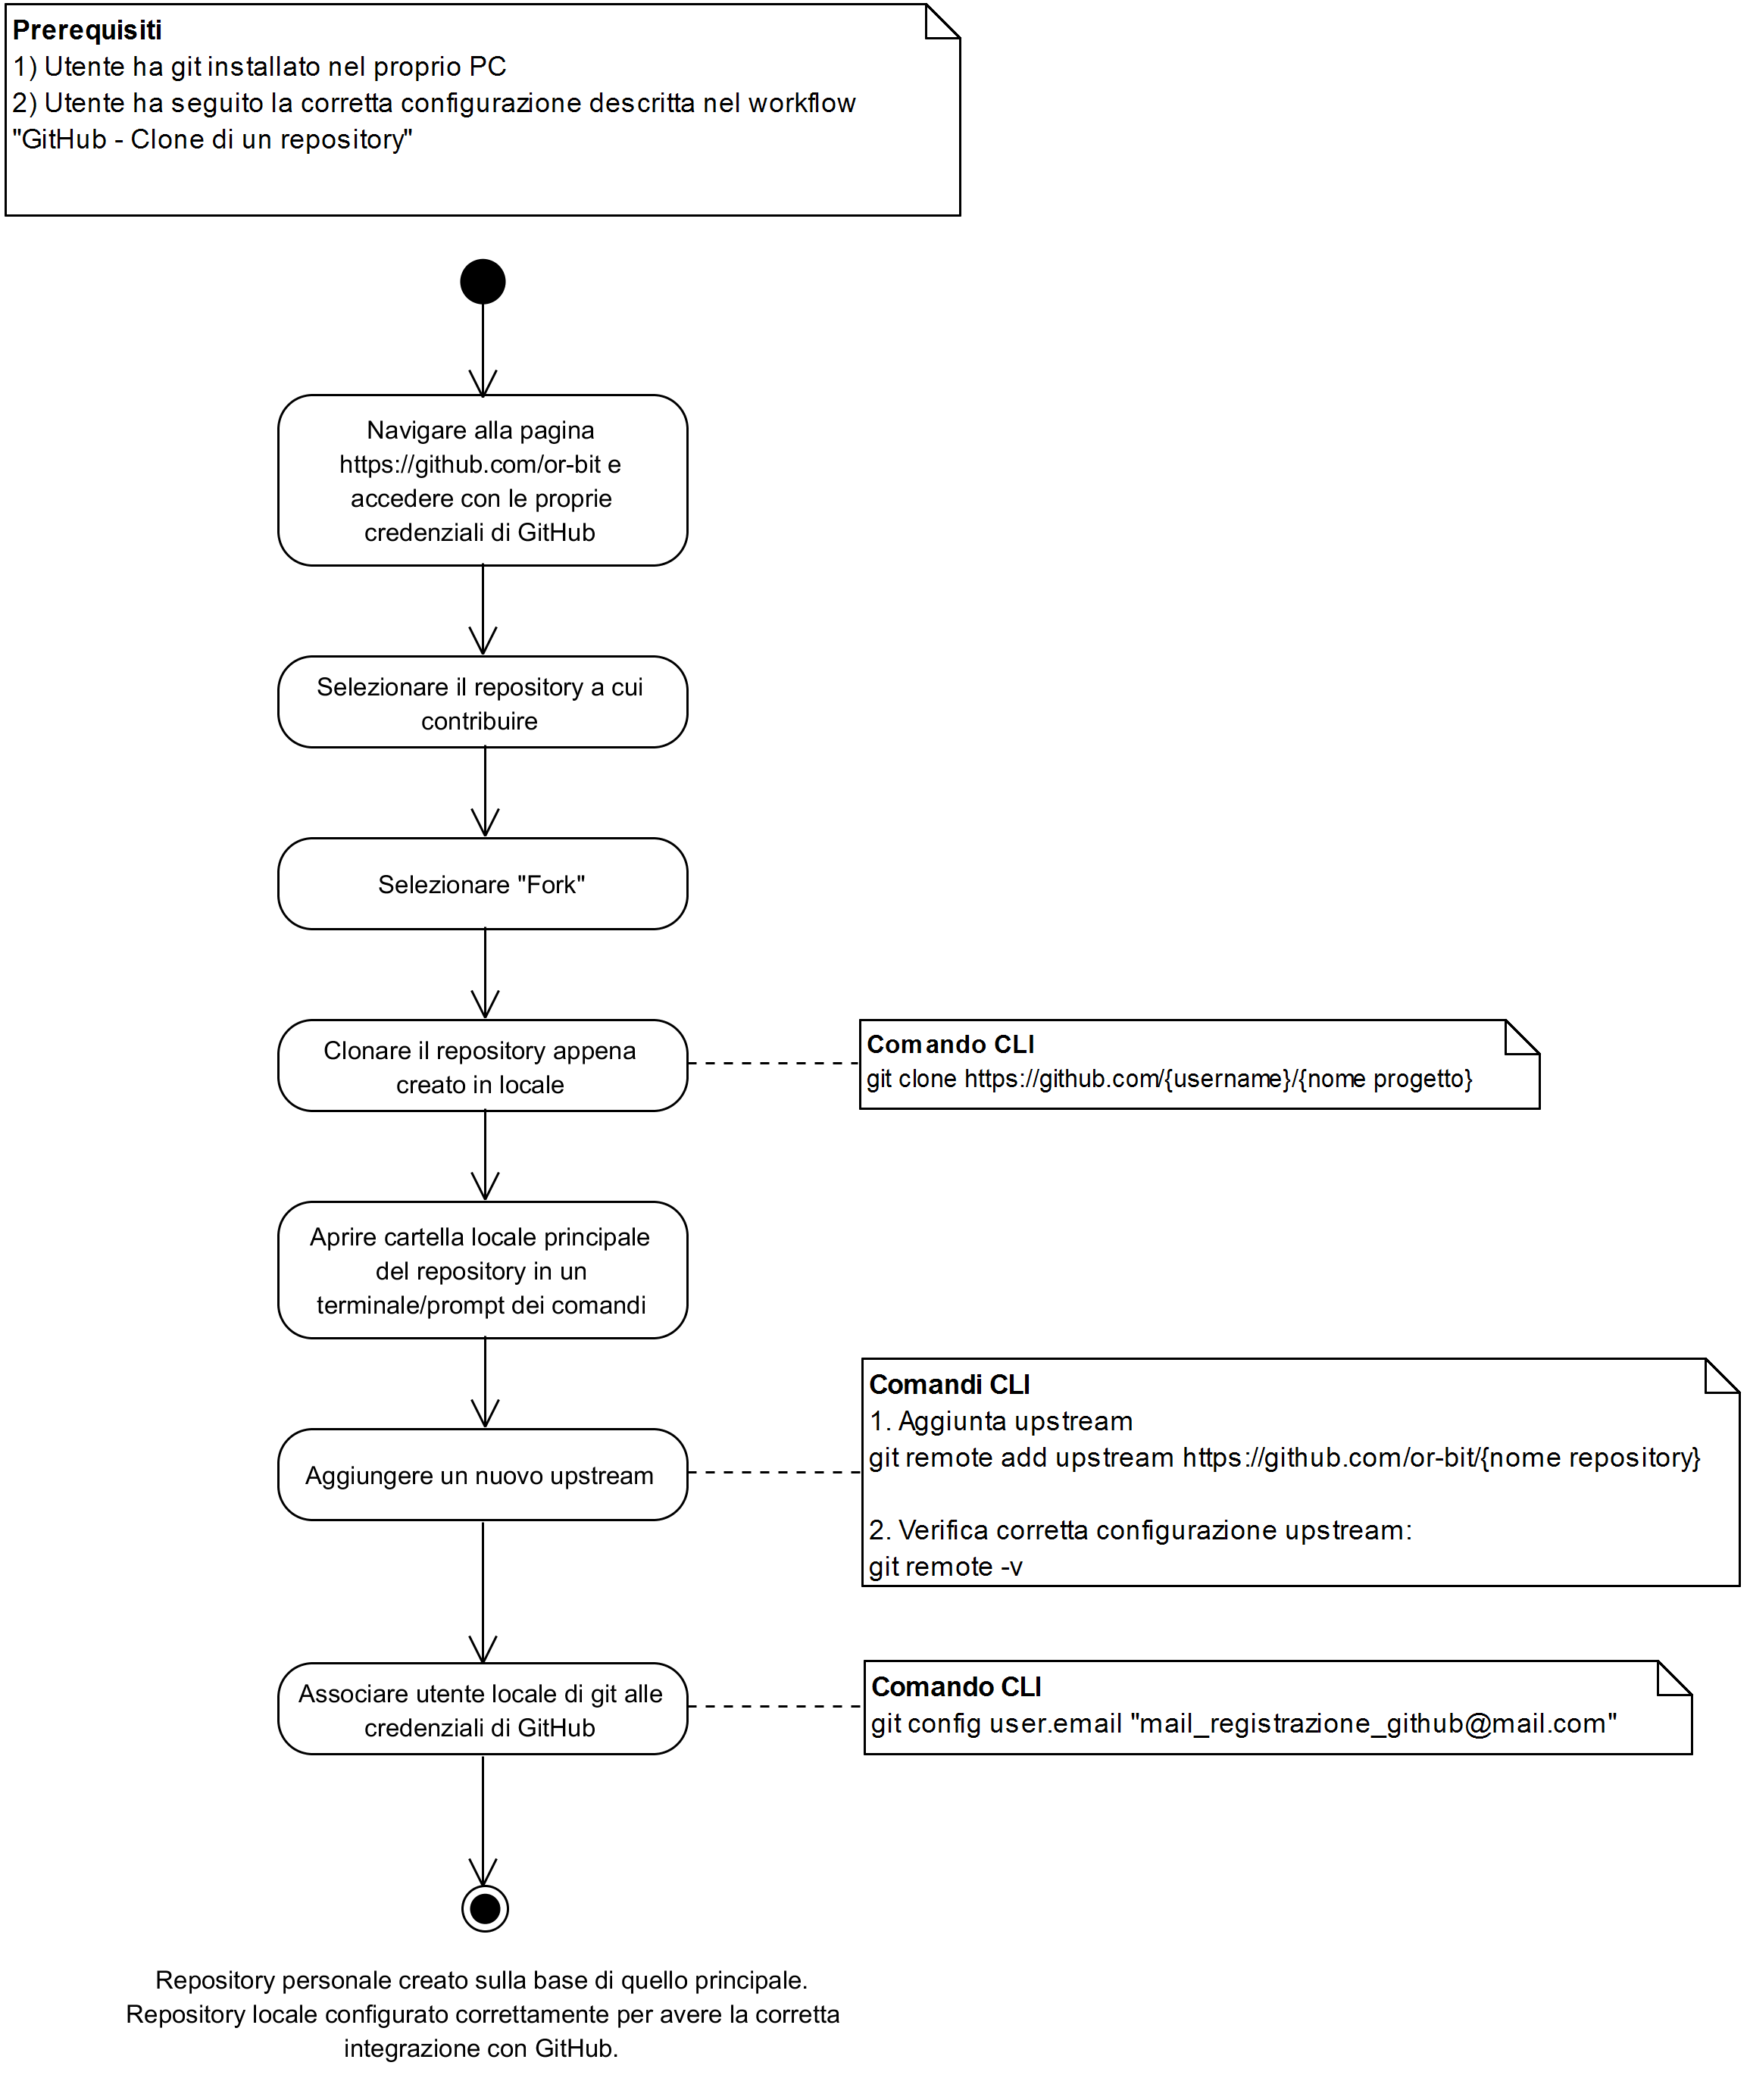
\includegraphics[width=15cm]{../../documenti/NormeDiProgetto/DiagrammiProcedure/GitHub-CloneDiUnRepository.png}
\captionof{figure}{Procedura di clonazione di un Repository}
\end{center}

\paragraph{Procedura di creazione di una Pull Request:}

\begin{center}
	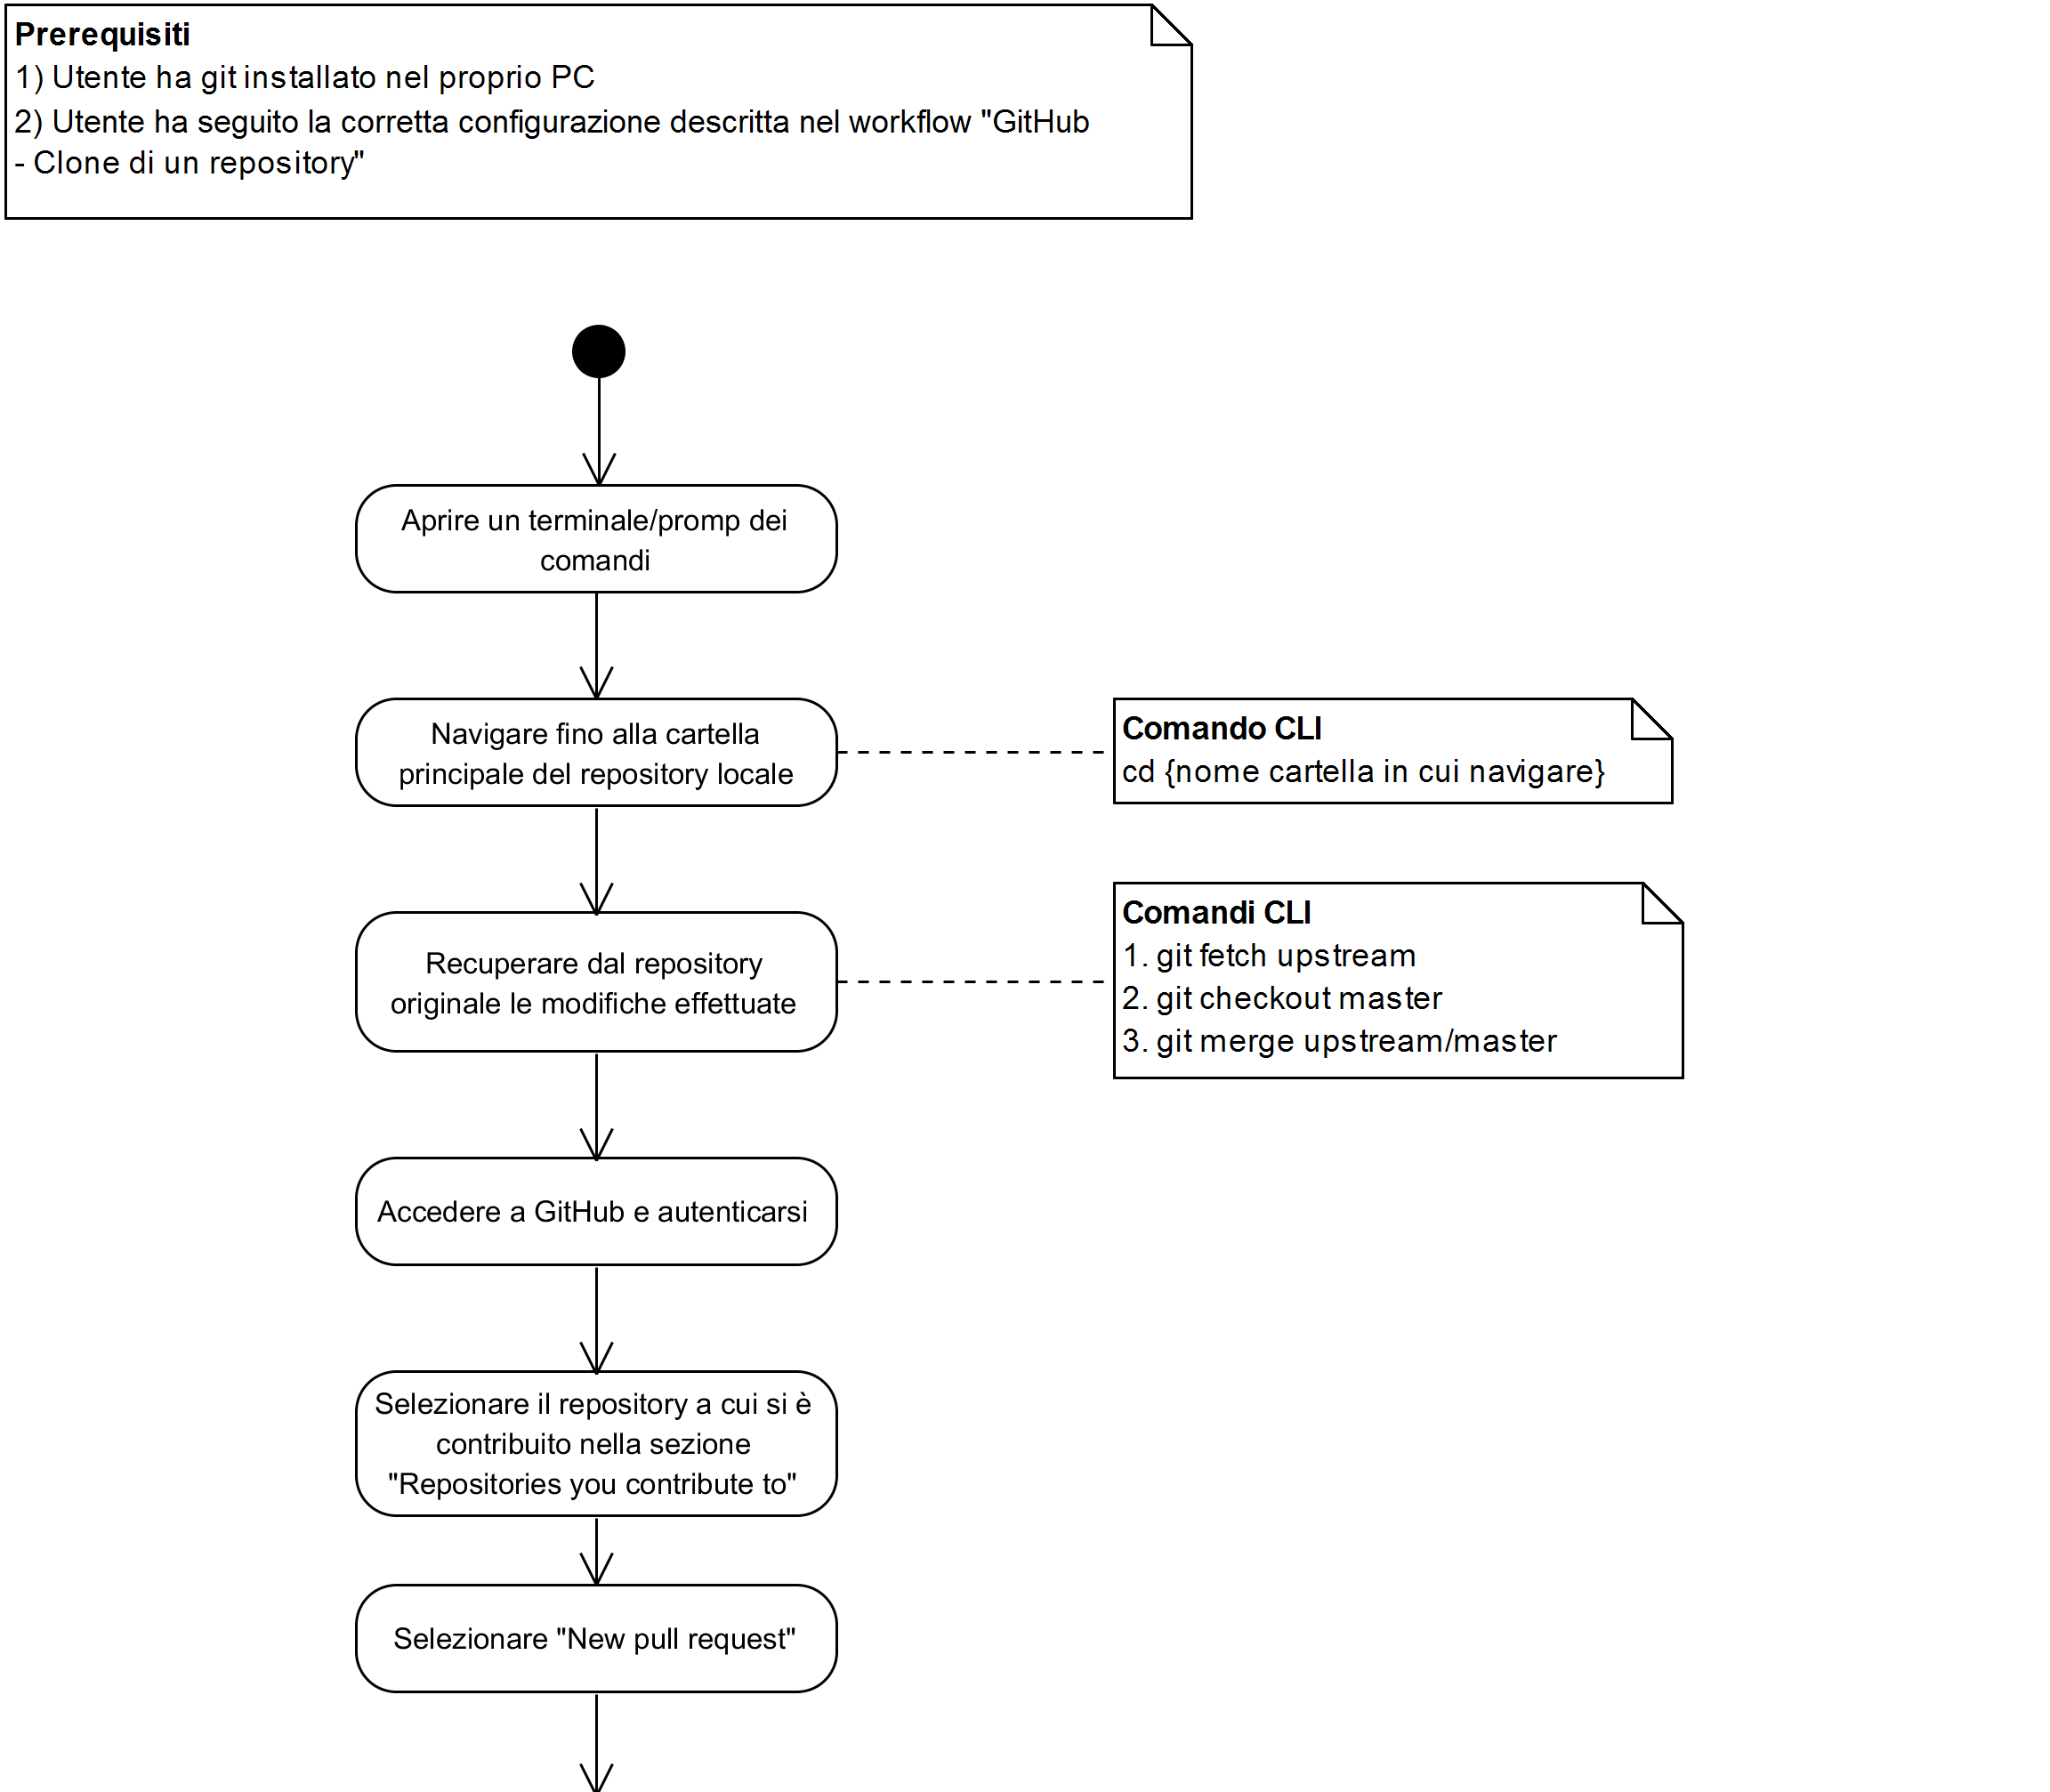
\includegraphics[width=15cm]{../../documenti/NormeDiProgetto/DiagrammiProcedure/GitHub-CreazionePullRequest1.png}
	\captionof{figure}{Procedura di creazione di una Pull Request parte 1}
\end{center}


\begin{center}
	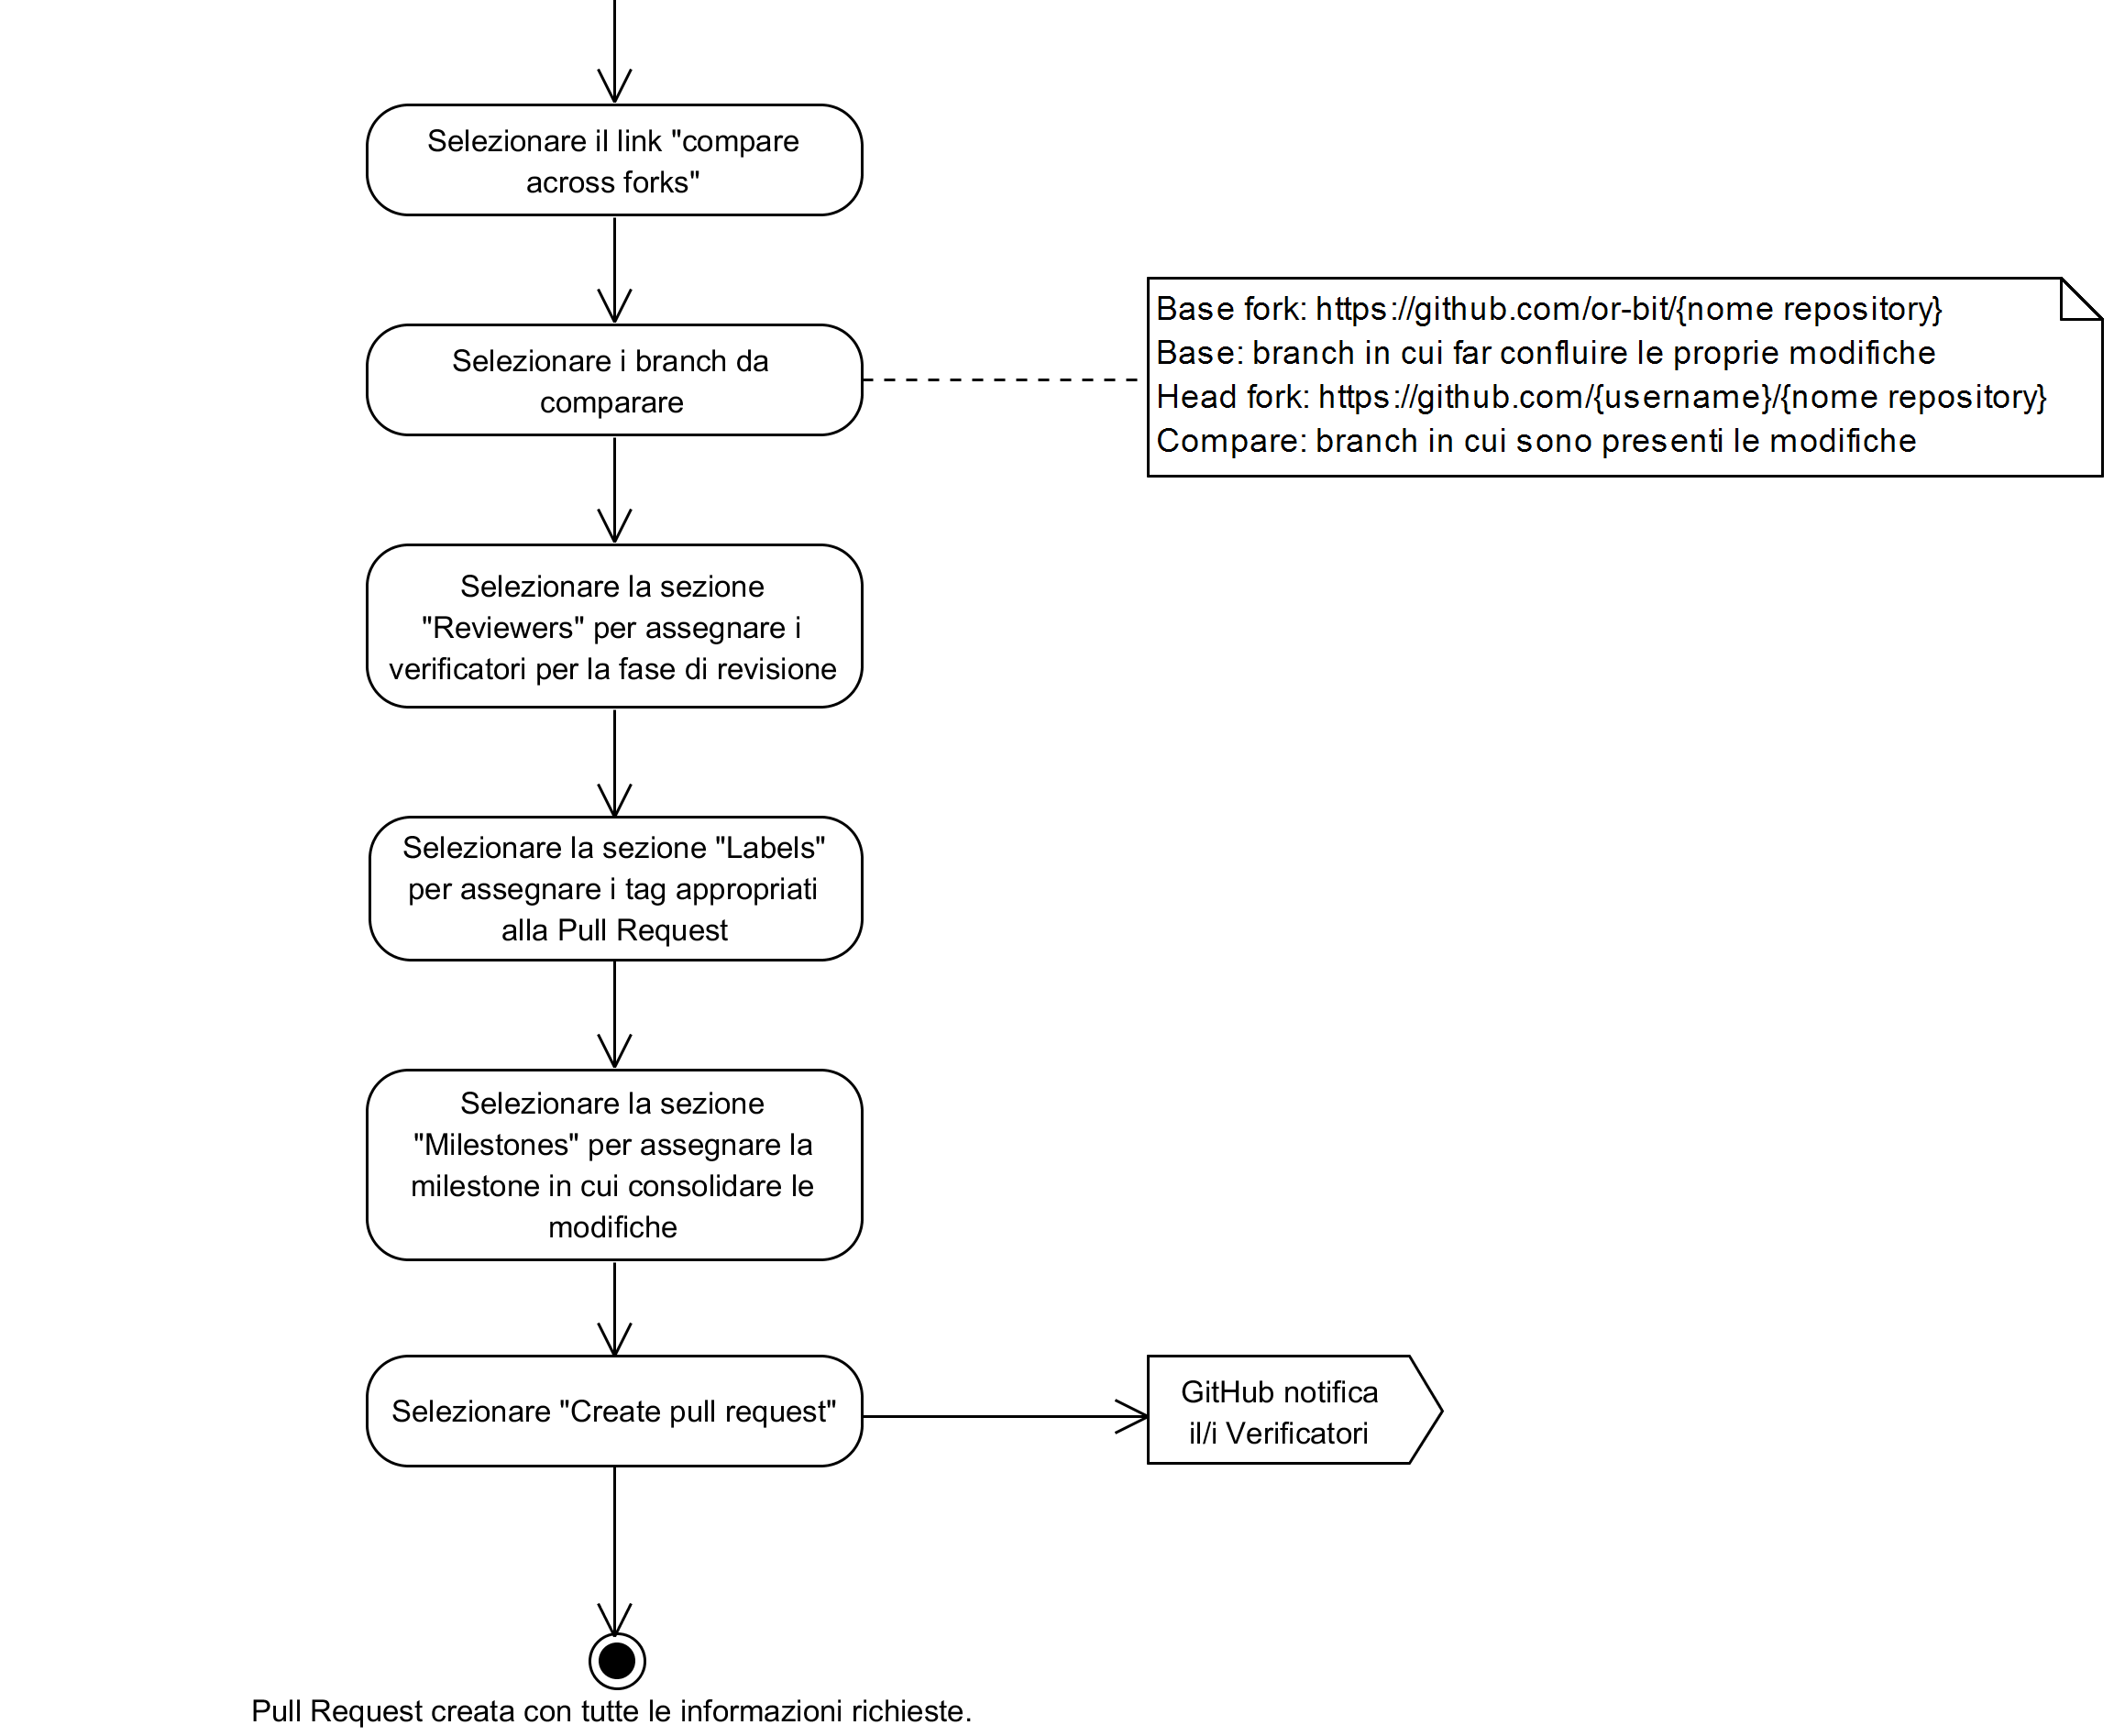
\includegraphics[width=15cm]{../../documenti/NormeDiProgetto/DiagrammiProcedure/GitHub-CreazionePullRequest2.png}
	\captionof{figure}{Procedura di creazione di una Pull Request parte 2}
\end{center}

\subsection{Software di integrazione continua}
Come software di integrazione continua viene utilizzato \textbf{\glossario{Travis}}.
\glossario{Travis} è un servizio open source sotto licenza \glossario{MIT}, quindi disponibile in versione gratuita, \glossario{hosted} ed integrabile con vari altri servizi, tra cui \glossario{GitHub} e \glossario{Heroku}.\\ \glossario{Travis} permette di produrre e testare progetti ospitati su \glossario{GitHub}. Ad ogni nuovo commit o pull request in \glossario{GitHub}, vengono quindi eseguiti specifici test e ne viene segnalato l'esito agli sviluppatori interessati. \glossario{Travis} è inoltre integrabile con strumenti e servizi esterni, per esempio per l'analisi statica.

\subsection{Software di pianificazione} \label{sec:teamwork}
Per la gestione e la pianificazione delle attività del progetto è stato scelto di utilizzare \textbf{\glossario{Teamwork Project}}. \glossario{Teamwork Project} è un programma web-based che permette la gestione completa di un progetto.\\
Esso fa parte del pacchetto \glossario{Teamwork} ed offre tutte le funzionalità richieste per la coordinazione ed il controllo delle attività.
\begin{itemize}
	\item \textbf{\glossario{Task}}:
	gestione chiara e intuitiva dei vari \glossario{task}, catalogabili per importanza, e delle dipendenze tra essi, anche attraverso sub\glossario{task}.\\
	I \glossario{task} sono assegnabili anche a più persone per consentire una distribuzione del lavoro efficace all'interno del team.
	
	\item \textbf{Time tracking}:
	\glossario{Teamwork} fornisce la possibilità di calcolare il tempo richiesto per effettuare un determinato \glossario{task} senza utilizzare altri strumenti. Questo permette di avere una visuale generale del tempo richiesto per ciascun \glossario{task} e quindi di organizzarsi al meglio per lo svolgimento delle diverse attività.
	
	\item \textbf{\glossario{Milestone}}:
	alle \glossario{milestone} possono essere associate liste di \glossario{task}, facilitando la comprensione dello stato di avanzamento delle attività relative a tali \glossario{milestone}.\\
	Le \glossario{milestone} possono essere assegnate a uno o più membri, dividendo in questo modo le responsabilità. Esse inoltre possono essere incorporate nel calendario: in questo modo i membri del gruppo interessati al completamento di una \glossario{milestone} vengono avvisati in prossimità della sua scadenza.
	
	\item \textbf{Diagrammi di \glossario{Gantt}}:	
	sono la rappresentazione grafica della pianificazione temporale delle attività, per studiare sequenzialità, parallelismo e interdipendenza tra \glossario{task} e relative scadenze.\\
	\glossario{Teamwork} genera in automatico questi diagrammi dalle liste di \glossario{task} create, agevolando il lavoro del \Responsabile.
	
	\item \textbf{Gestione riunioni}:
	\glossario{Teamwork} permette la creazione di riunioni con notifiche, reminder, e conferma di partecipazione.
	
	\item \textbf{Gestione pagamenti}:
	tracciamento dei costi di progetto, valutando il costo unitario a seconda dei ruoli e del lavoro svolto.
\end{itemize}

\newpage
\subsubsection{Modalità di utilizzo} \label{sec:procedure_teamwork}

\paragraph{Procedura di creazione di un evento:}

\begin{center}
	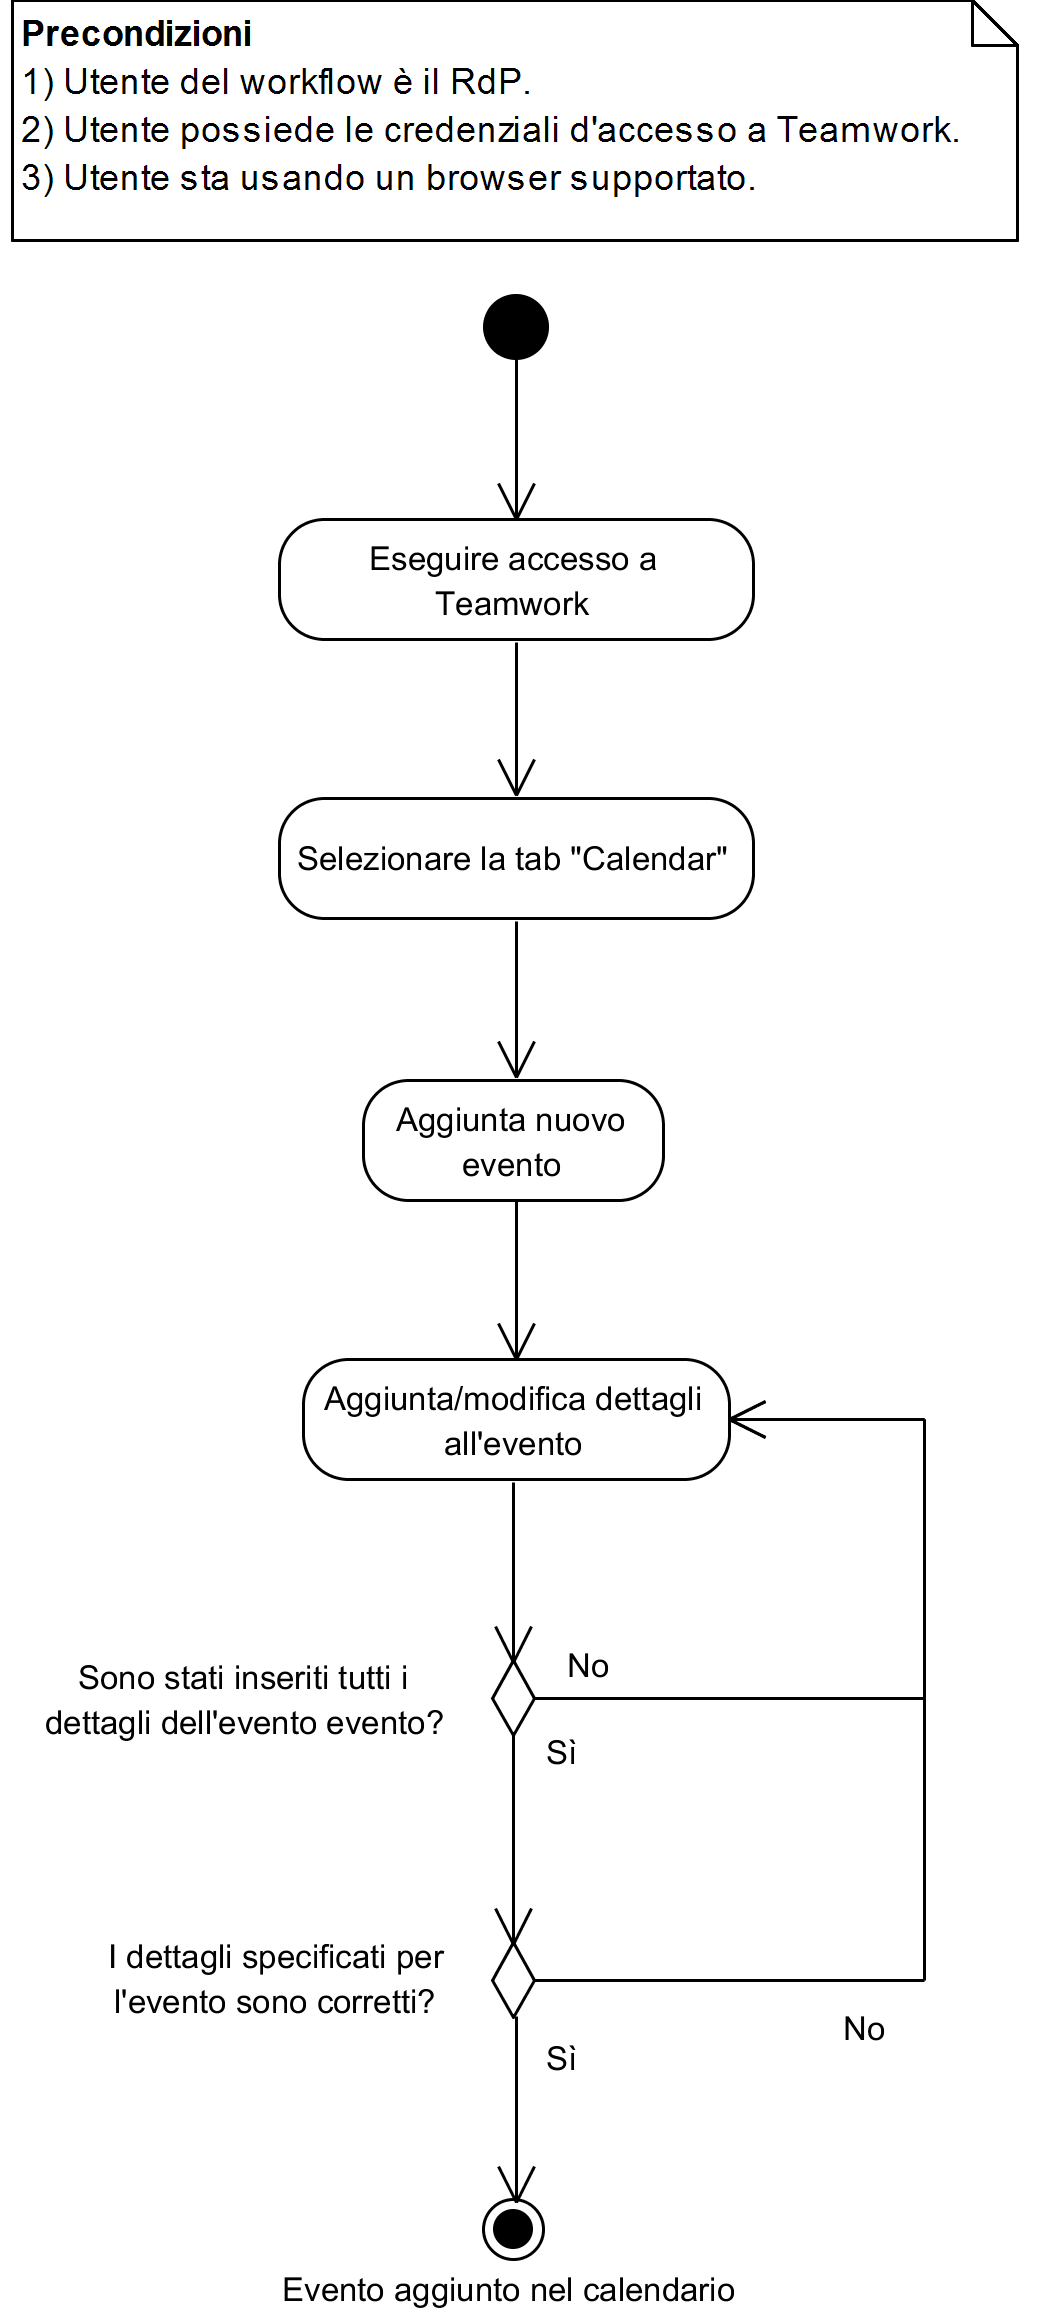
\includegraphics[width=8cm]{../../documenti/NormeDiProgetto/DiagrammiProcedure/CreazioneEventoNelCalendario.png}
	\captionof{figure}{Procedura di creazione di un evento}
\end{center}

\paragraph{Procedura di creazione di una Milestone:}

\begin{center}
	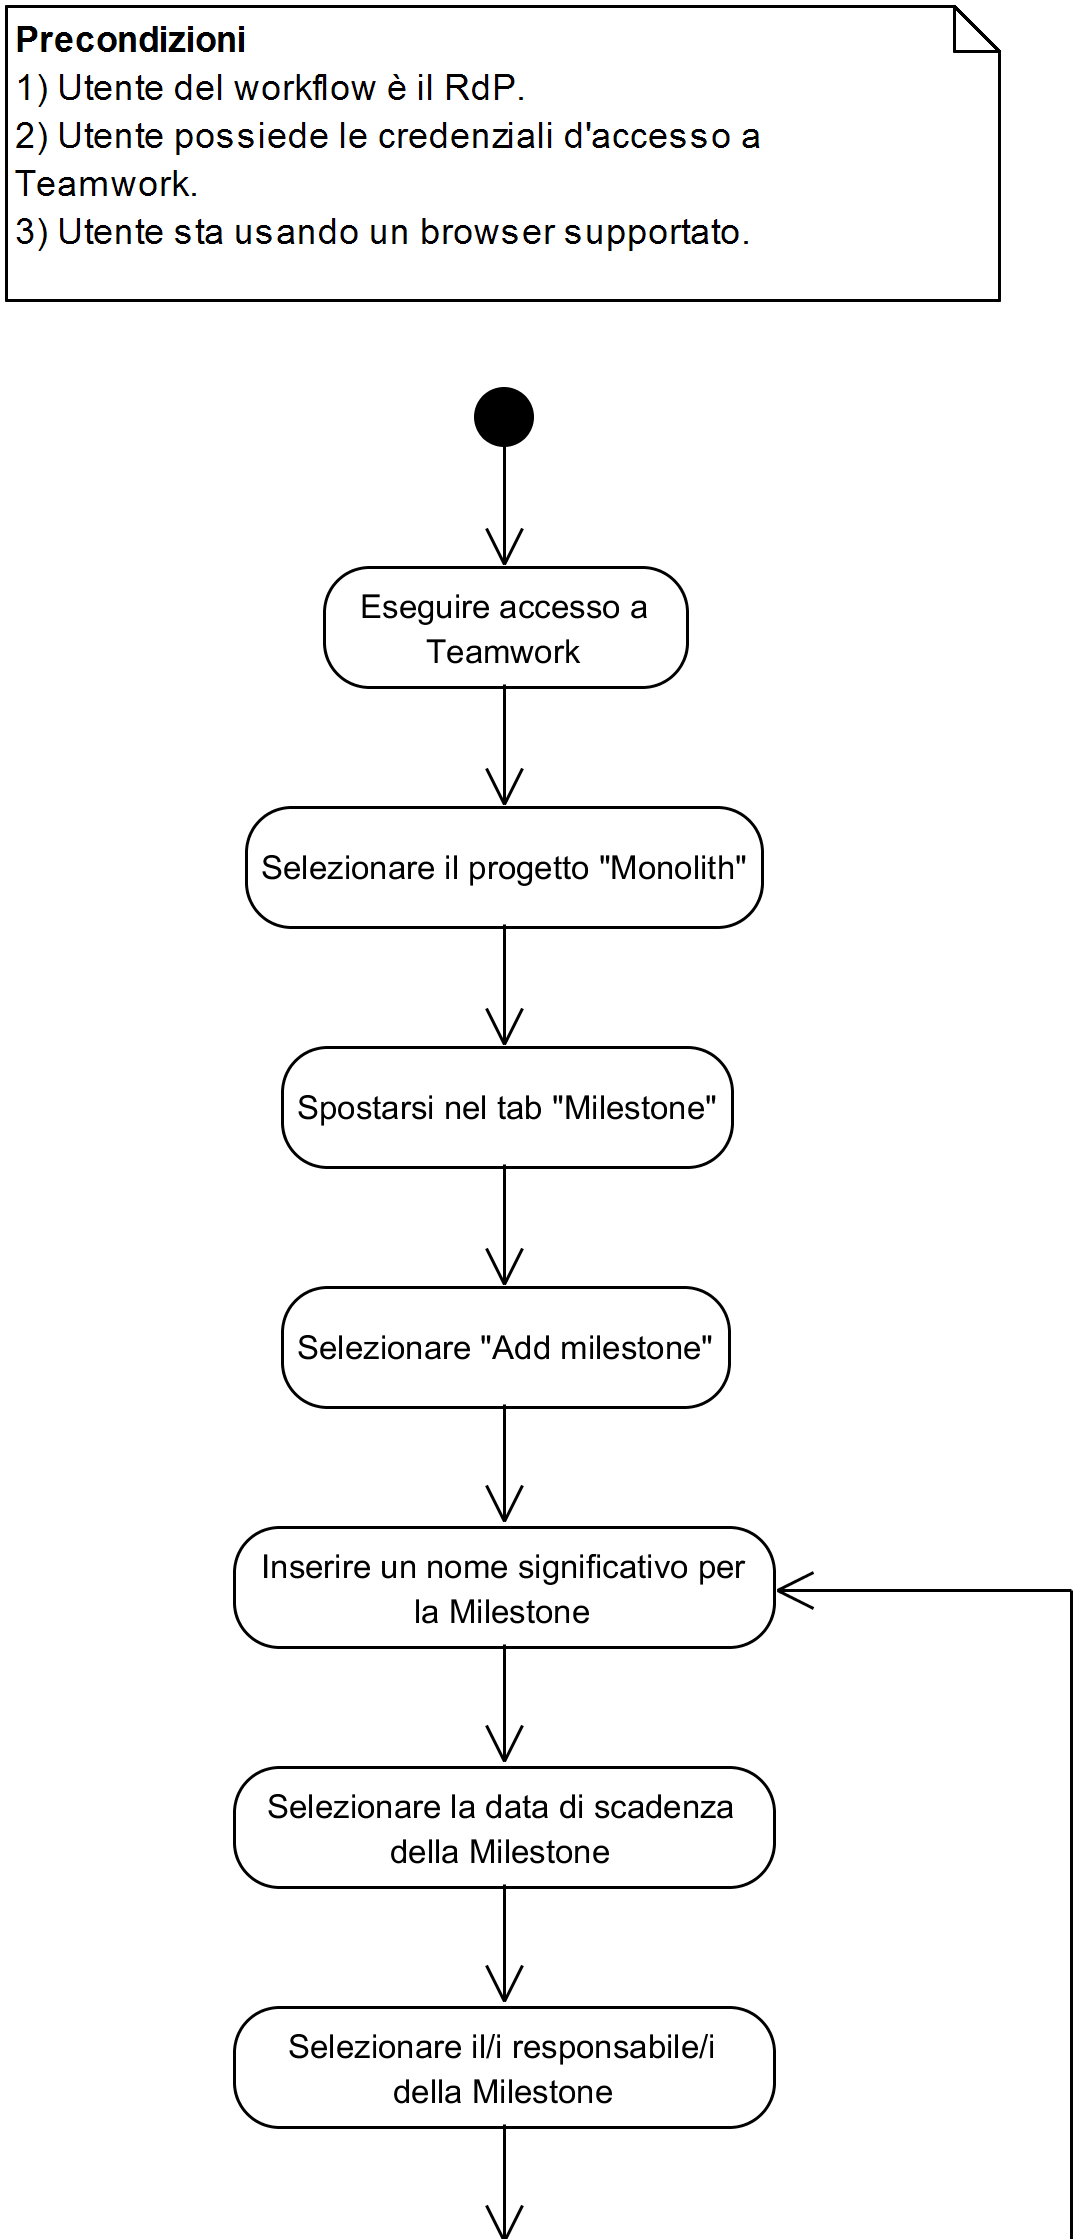
\includegraphics[width=8cm]{../../documenti/NormeDiProgetto/DiagrammiProcedure/CreazioneMilestone1.png}
	\captionof{figure}{Procedura di creazione di una \glossario{Milestone} parte 1}
\end{center}

\begin{center}
	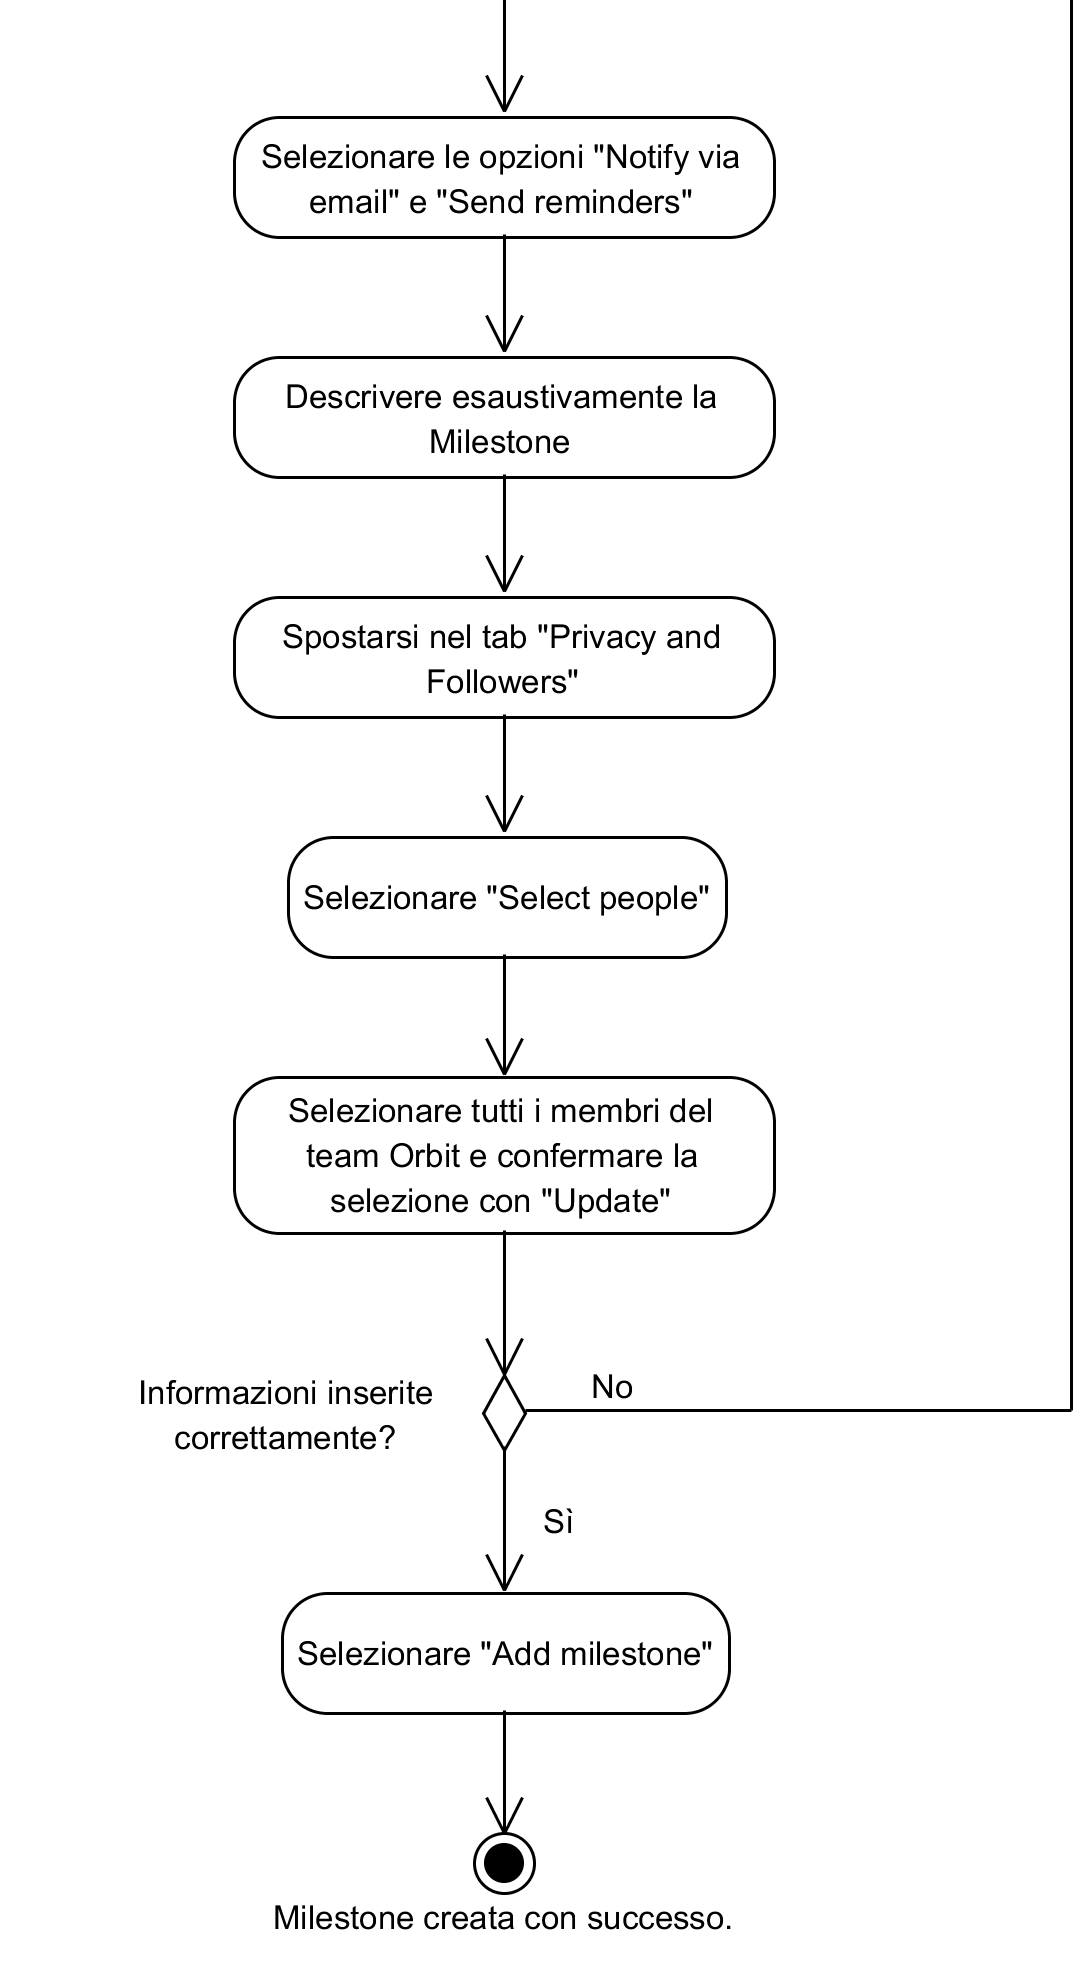
\includegraphics[width=8cm]{../../documenti/NormeDiProgetto/DiagrammiProcedure/CreazioneMilestone2.png}
	\captionof{figure}{Procedura di creazione di una \glossario{Milestone} parte 2}
\end{center}

\newpage
\paragraph{Procedura di creazione di un Task:}

\begin{center}
	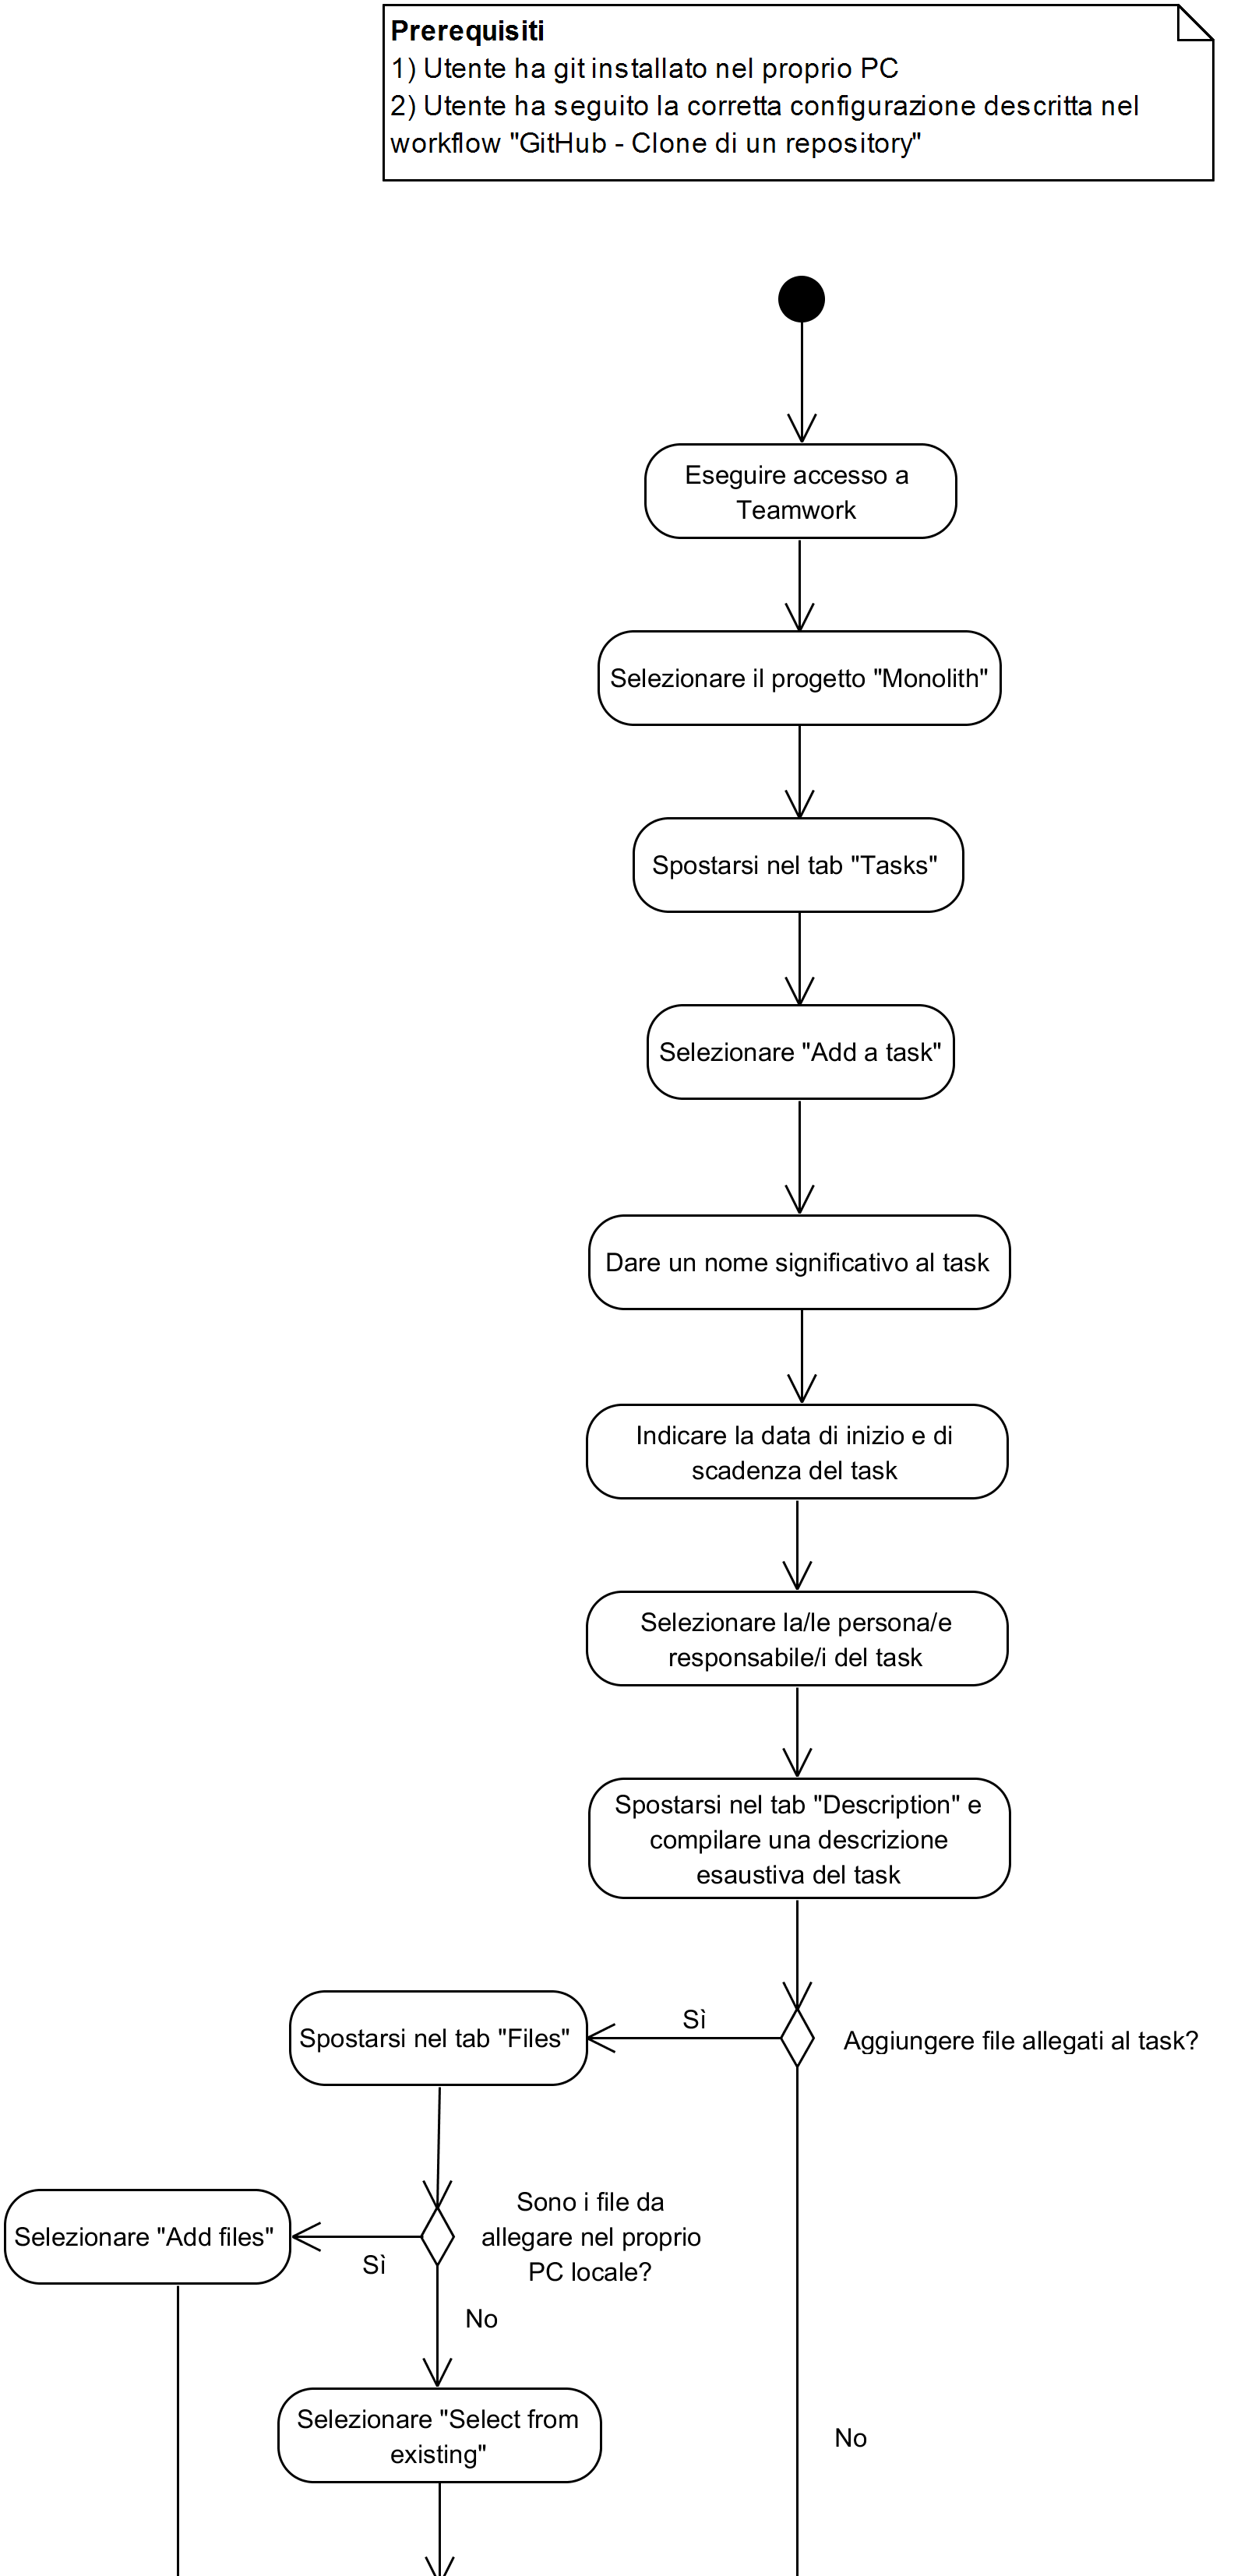
\includegraphics[width=9cm]{../../documenti/NormeDiProgetto/DiagrammiProcedure/CreazioneTask1.png}
	\captionof{figure}{Procedura di creazione di un Task parte 1}
\end{center}

\begin{center}
	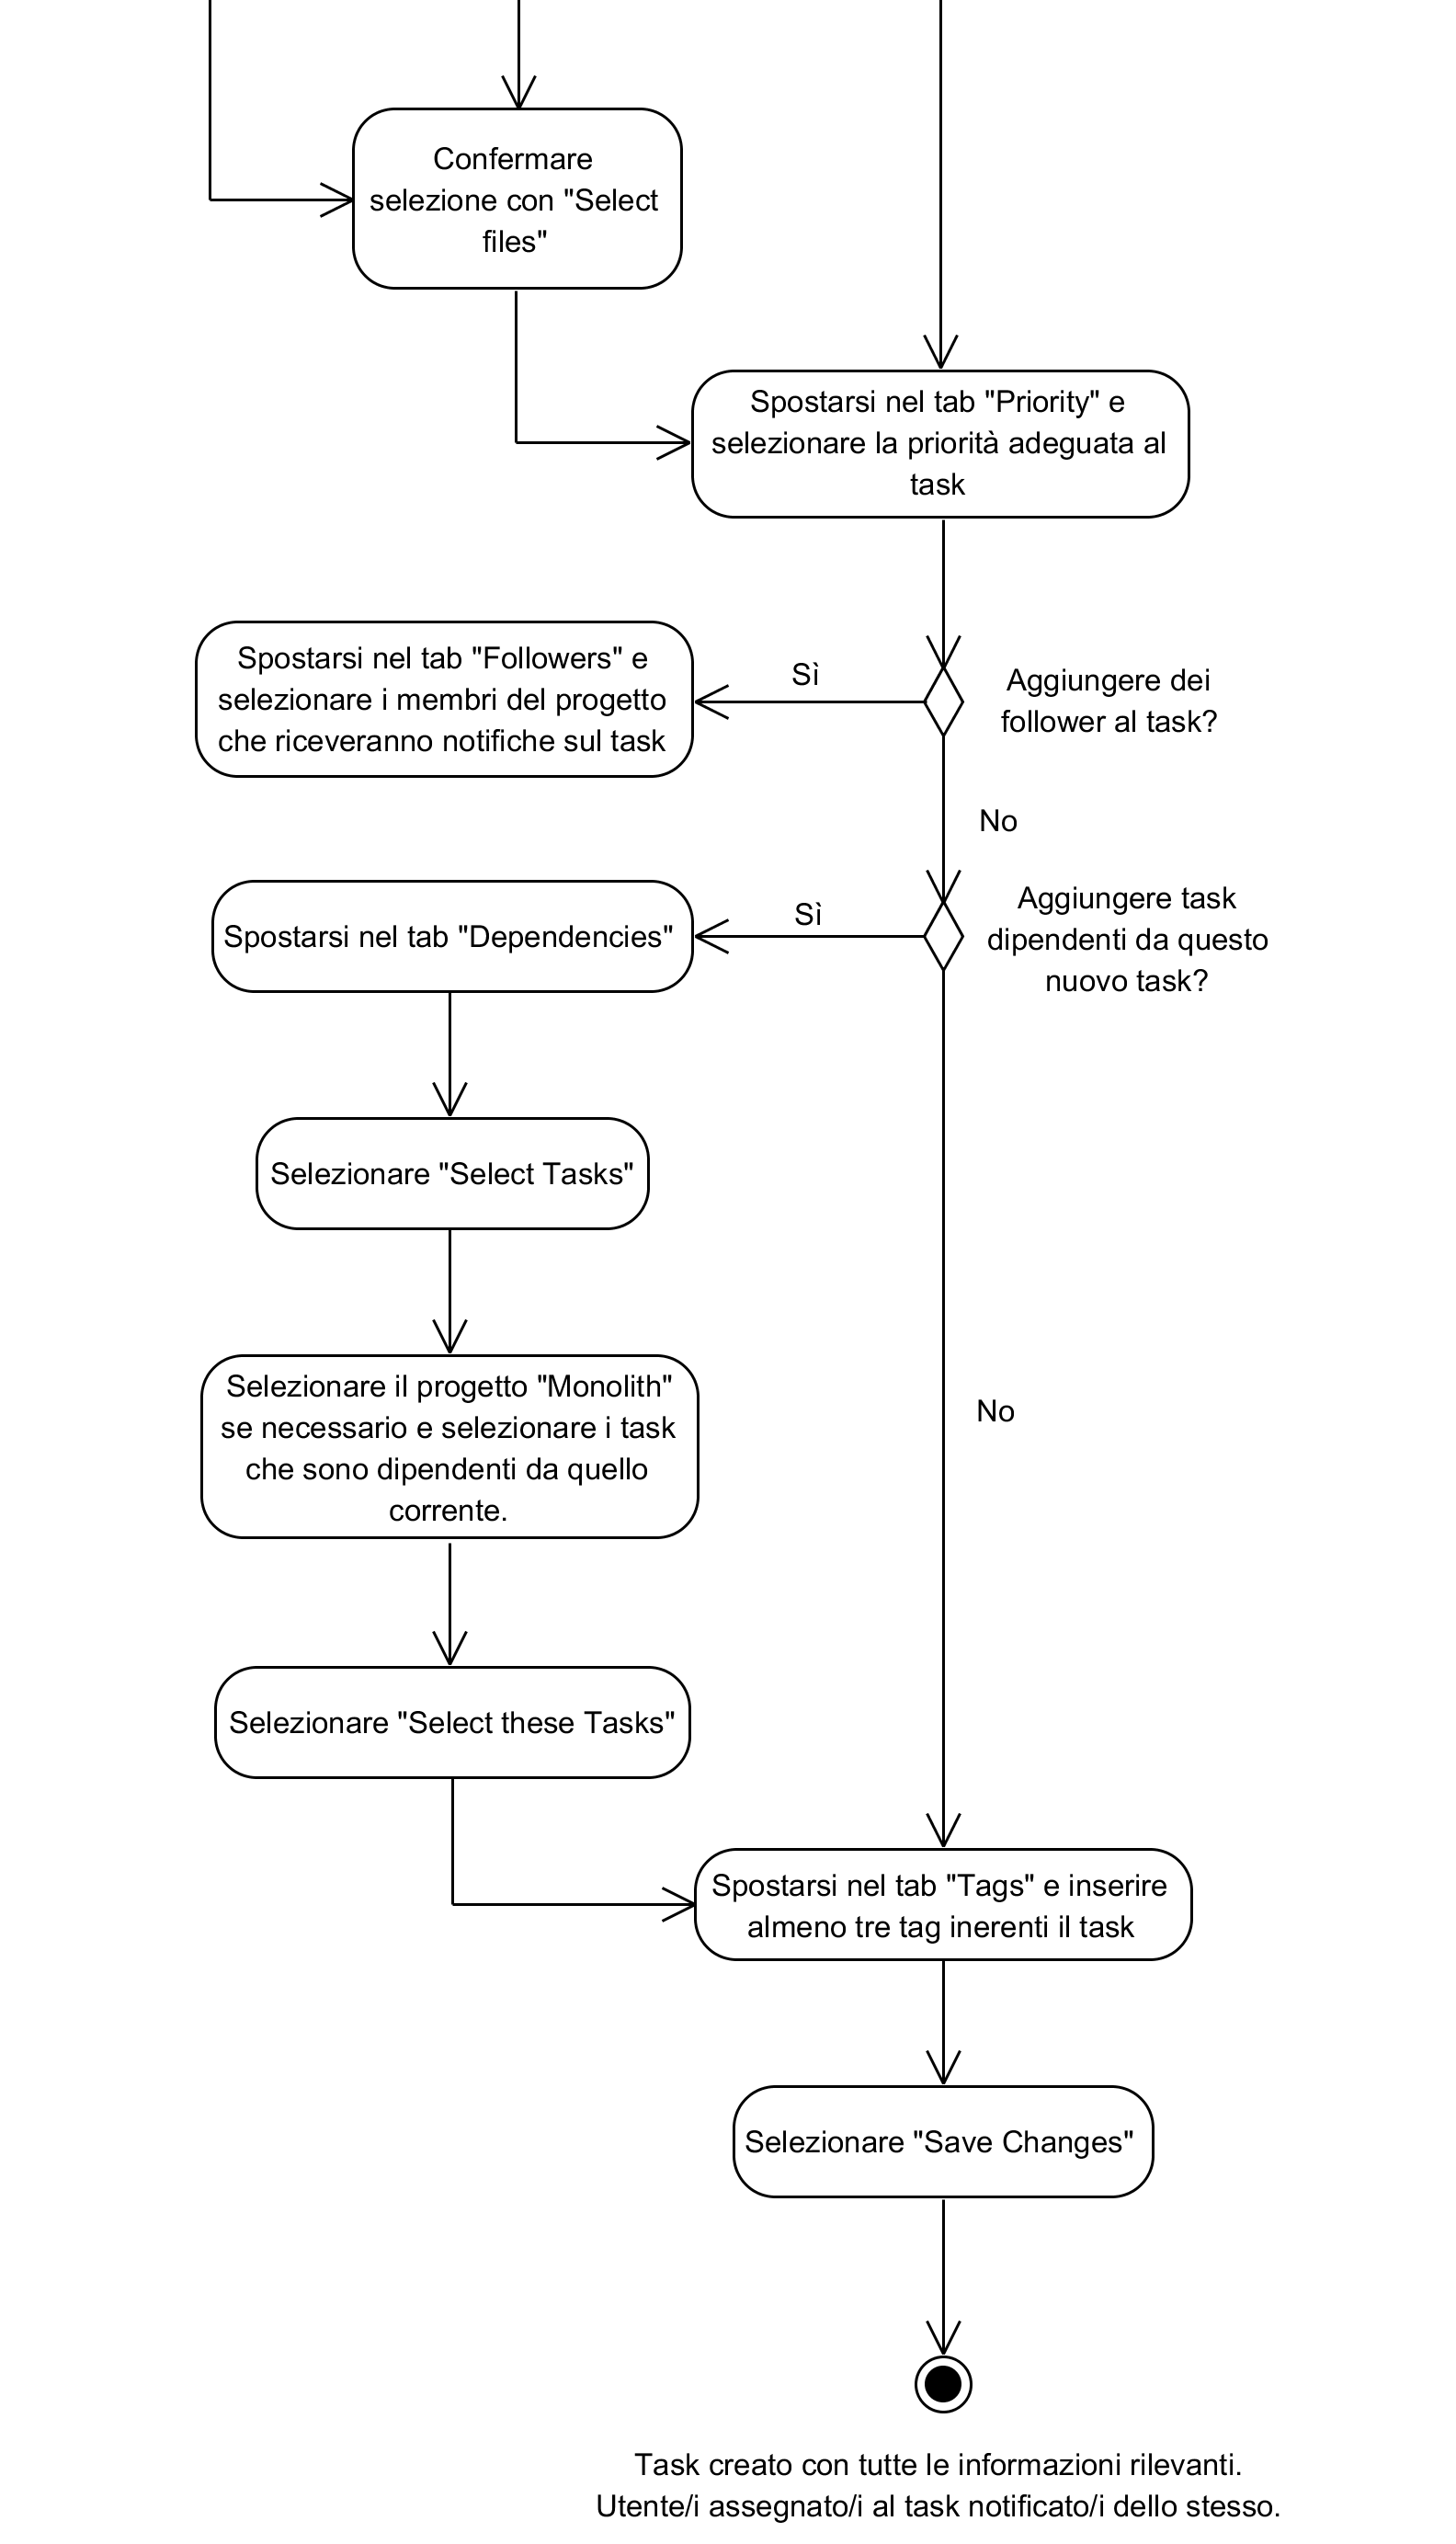
\includegraphics[width=11cm]{../../documenti/NormeDiProgetto/DiagrammiProcedure/CreazioneTask2.png}
	\captionof{figure}{Procedura di creazione di un Task parte 2}
\end{center}

\newpage
\paragraph{Procedura di modifica di un evento:}

\begin{center}
	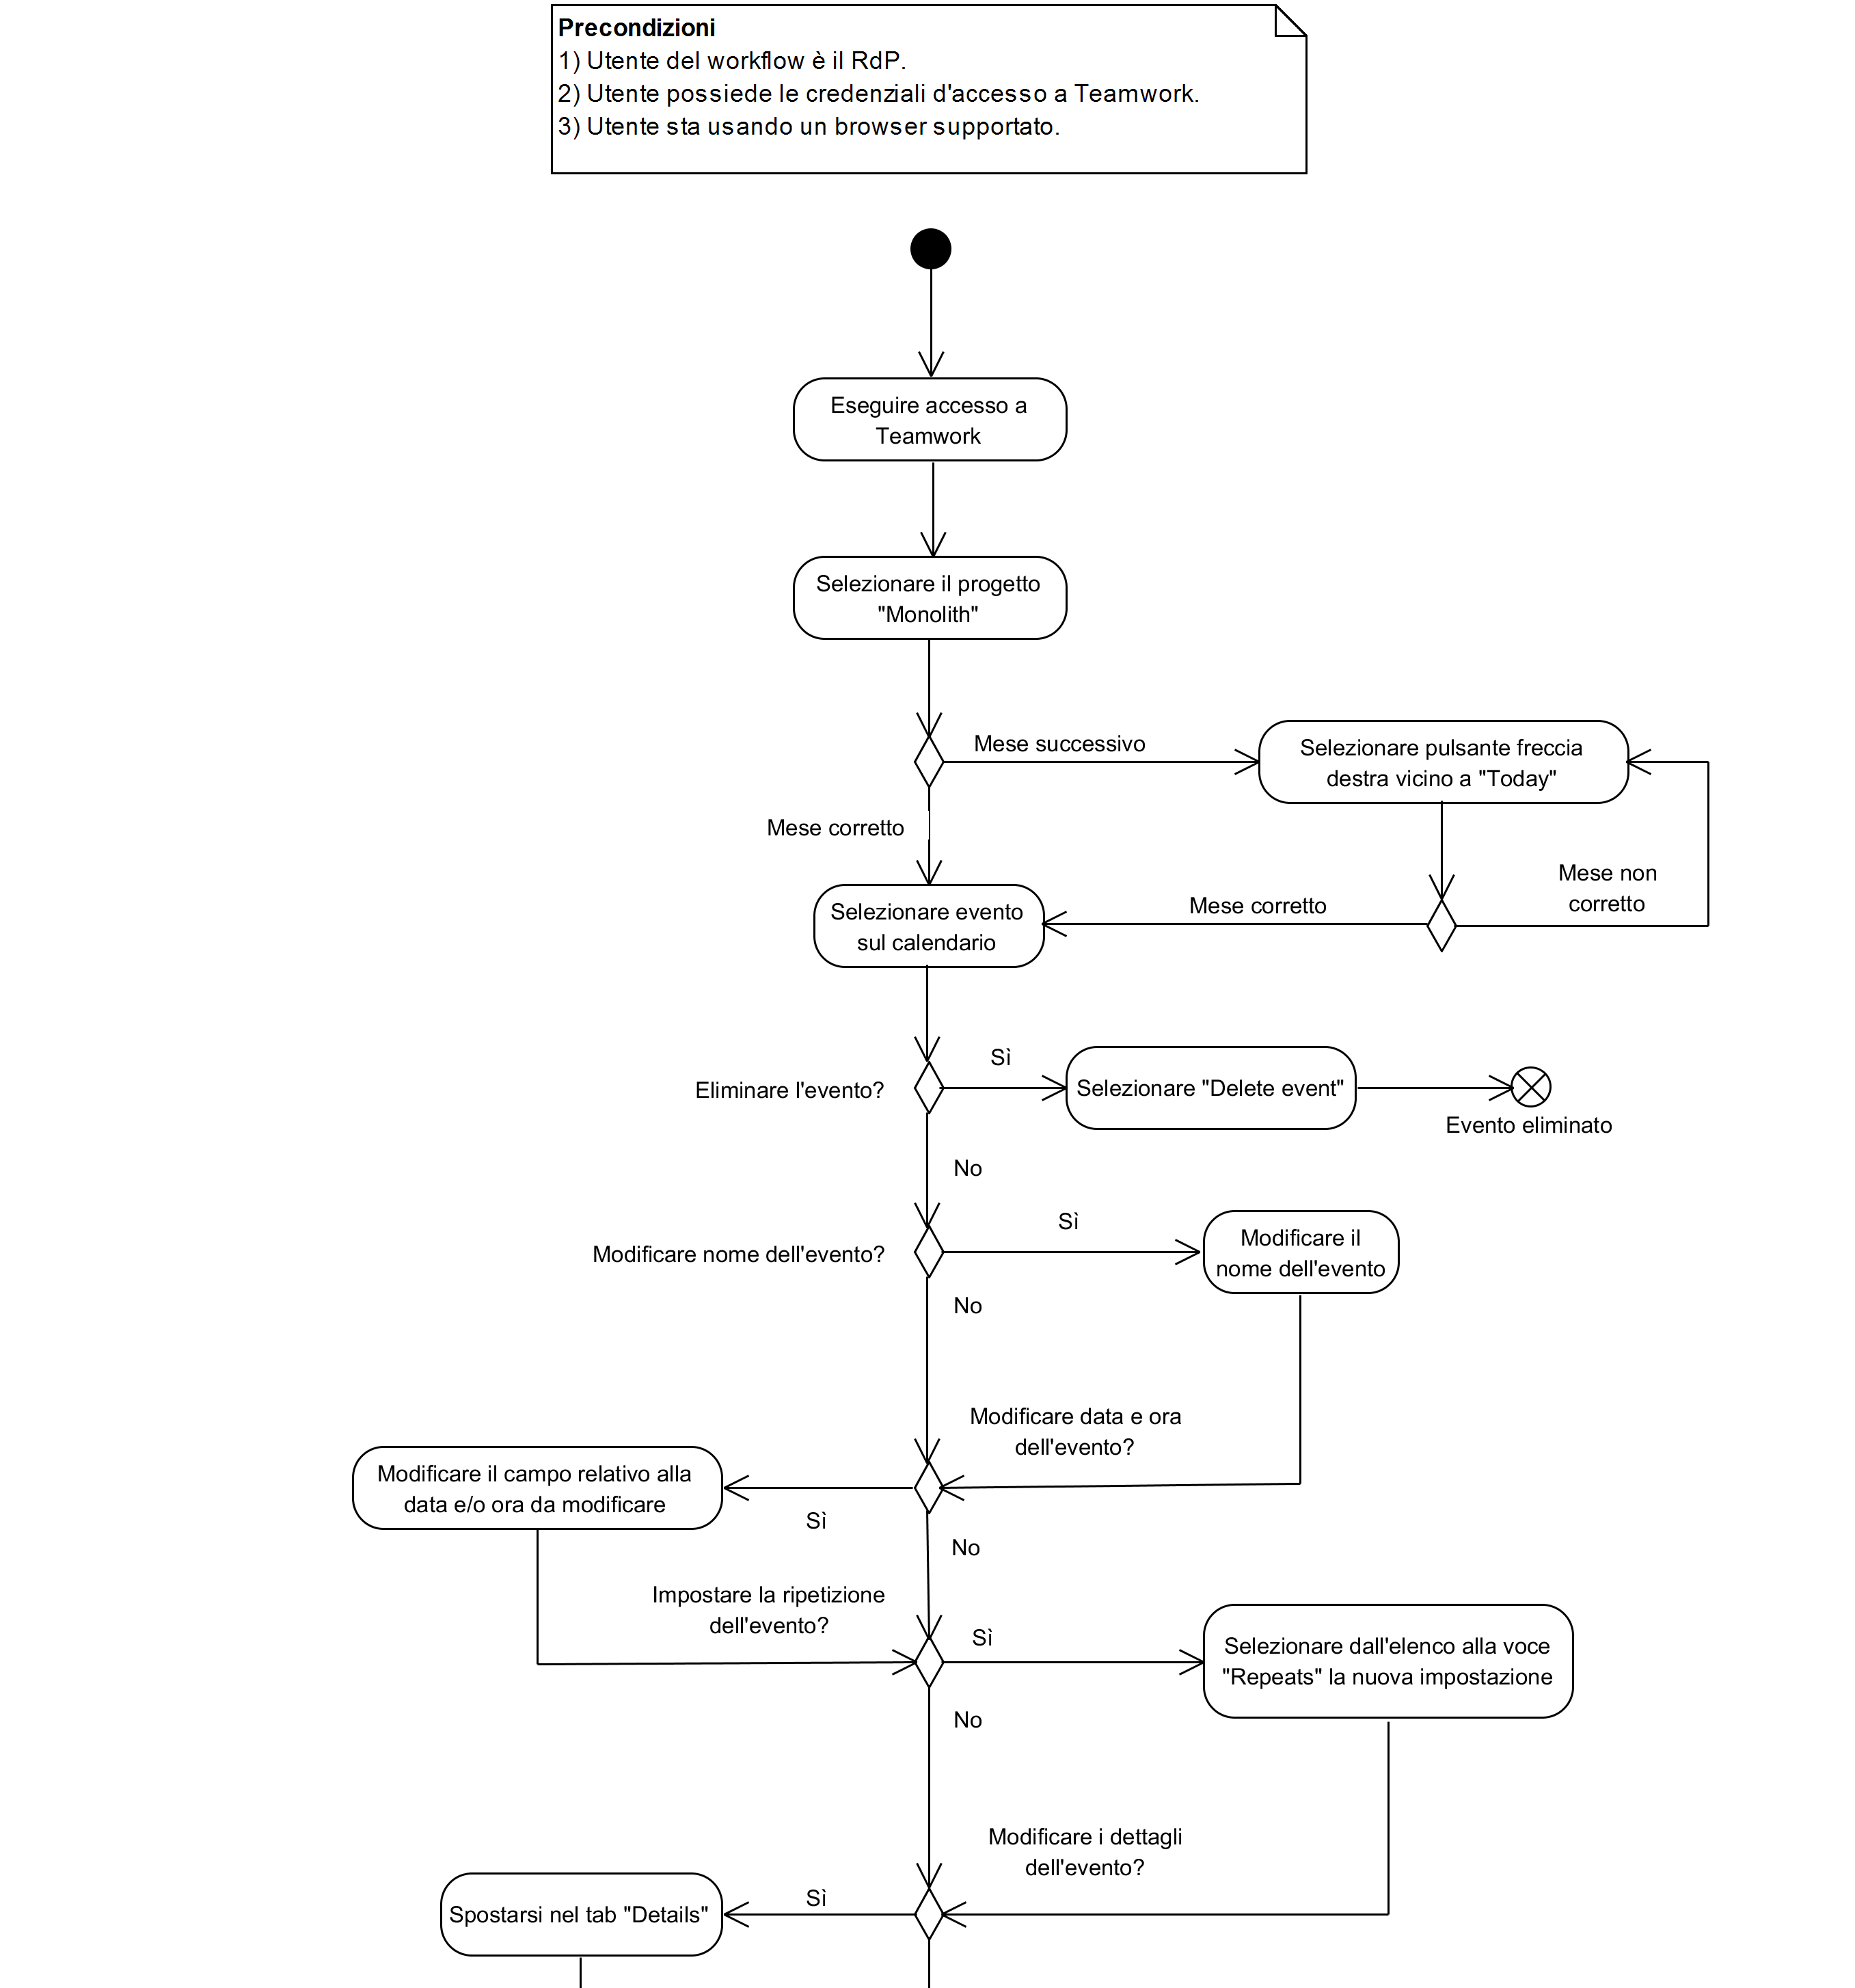
\includegraphics[width=15cm]{../../documenti/NormeDiProgetto/DiagrammiProcedure/EditEventi1.png}
	\captionof{figure}{Procedura di modifica di un evento - Inizio}
\end{center}

\begin{center}
	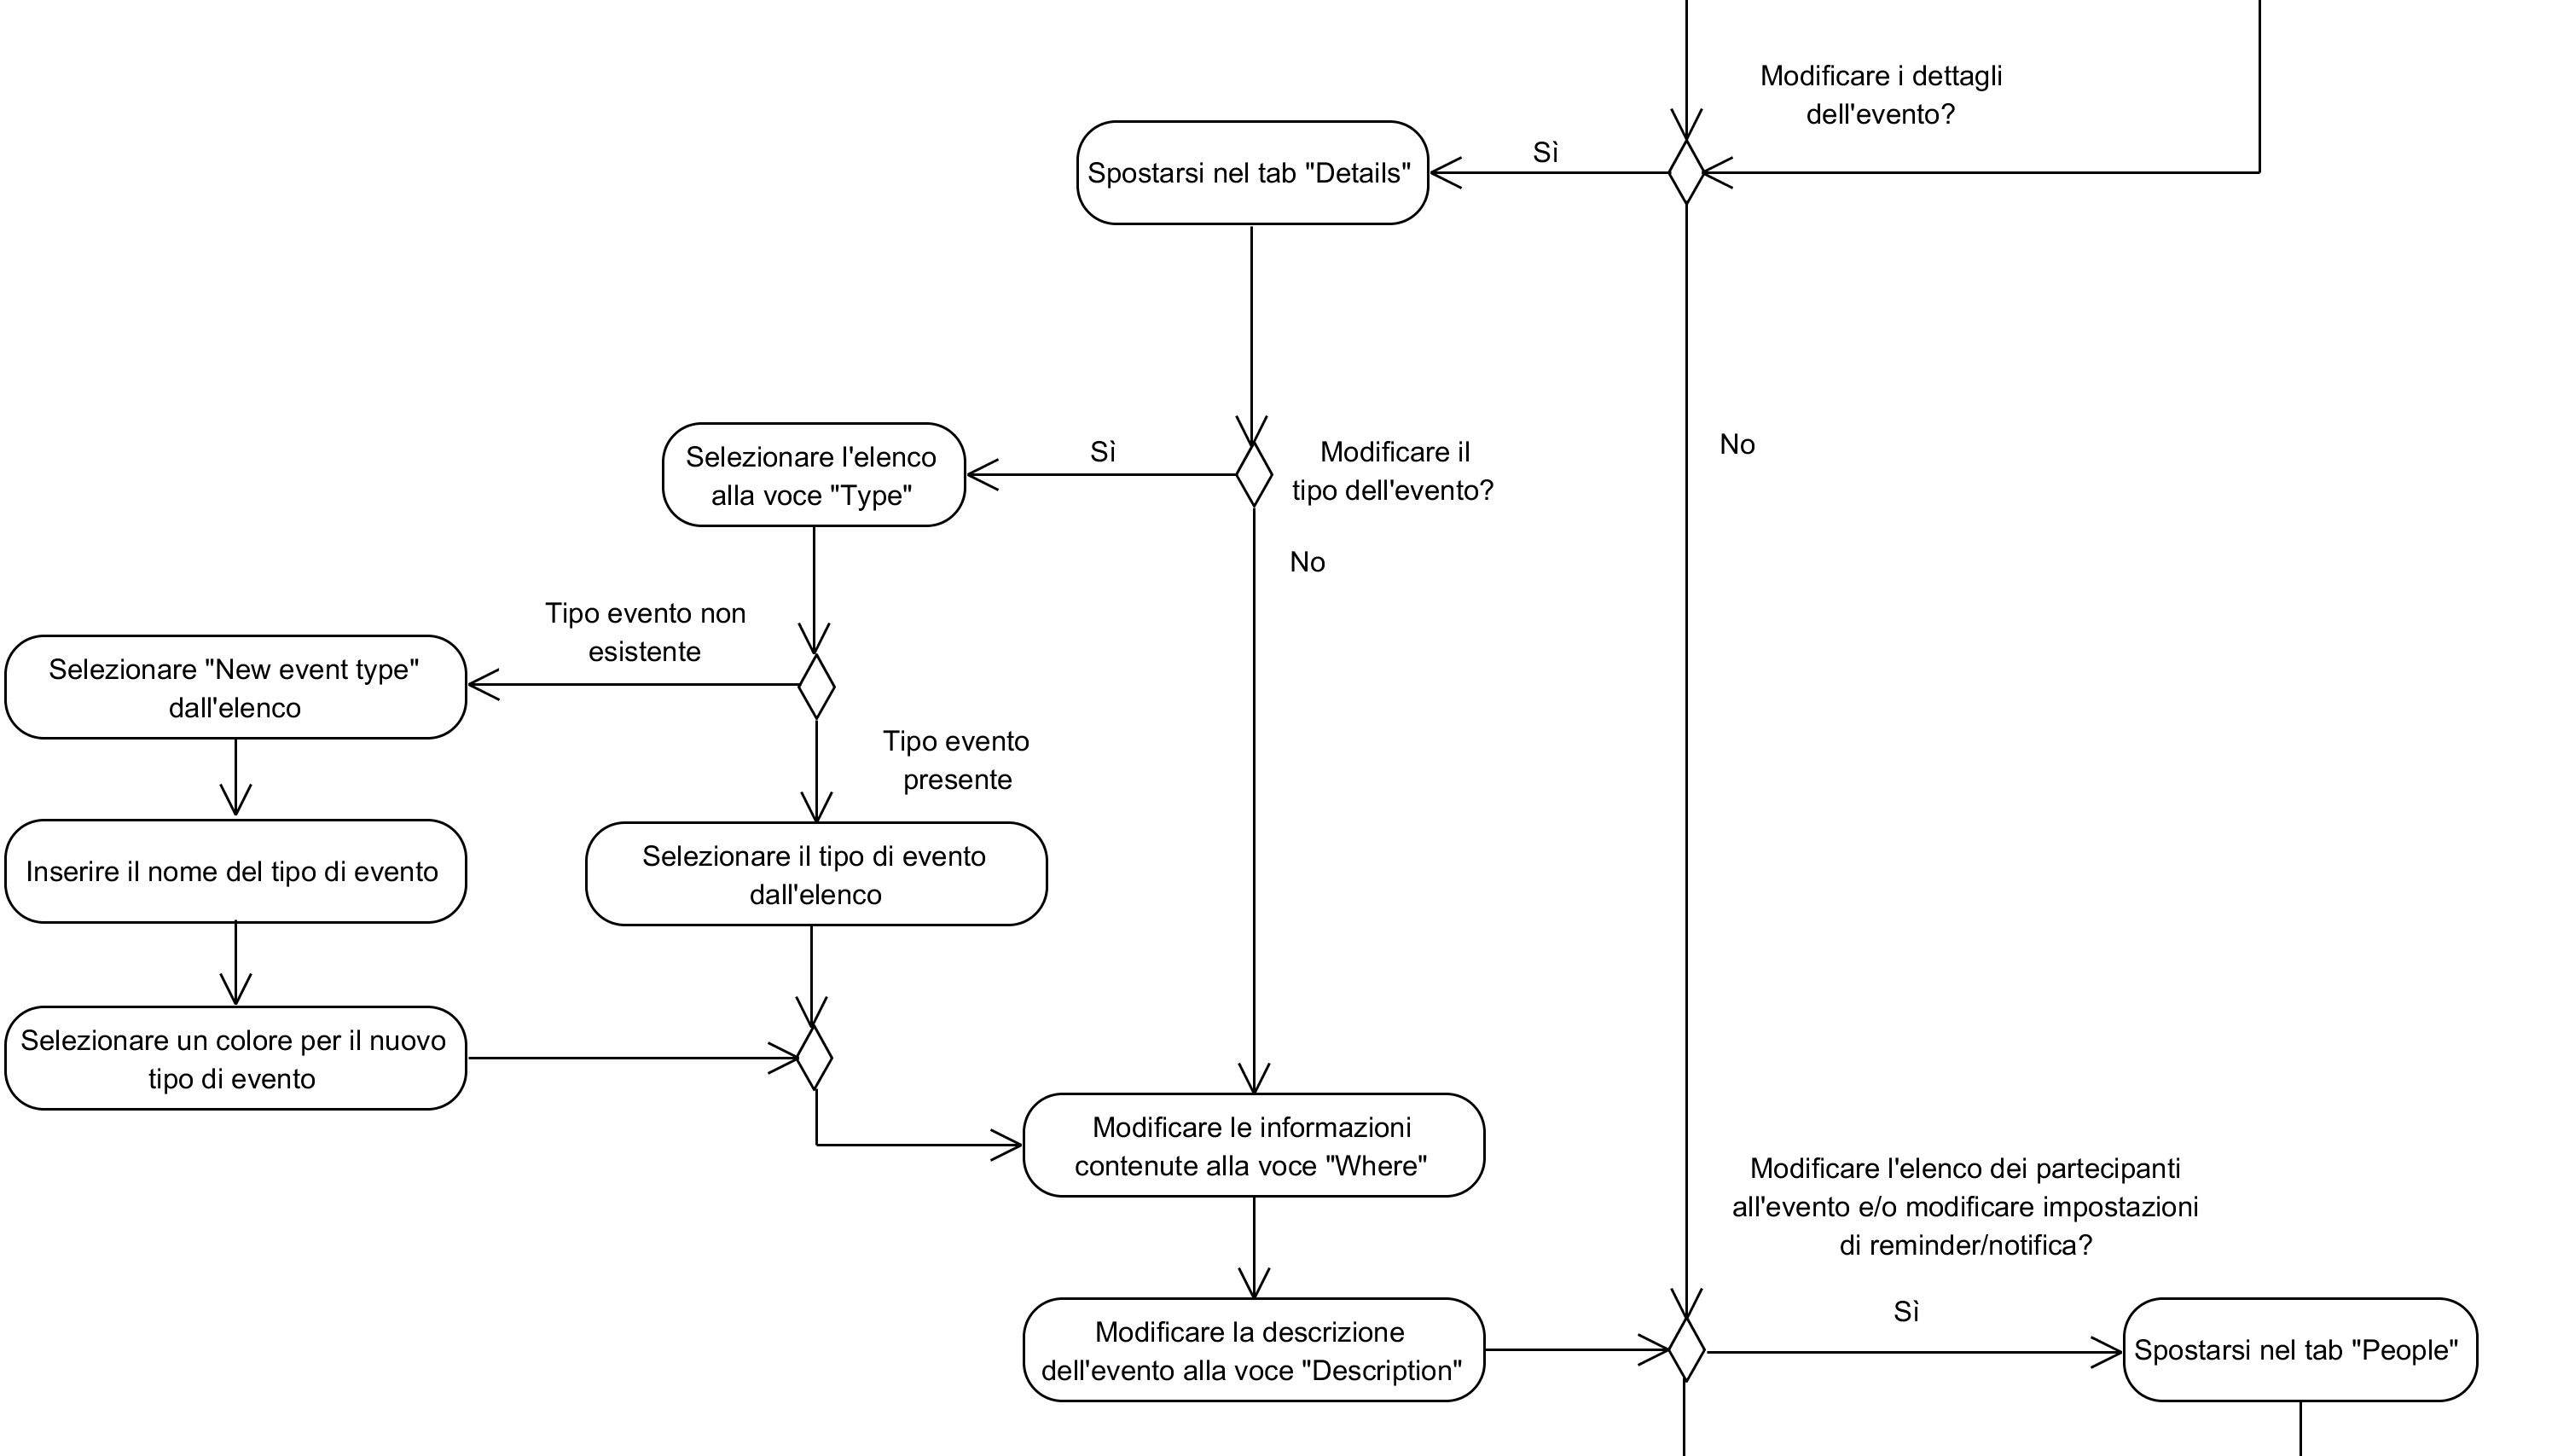
\includegraphics[width=15cm]{../../documenti/NormeDiProgetto/DiagrammiProcedure/EditEventi2.png}
	\captionof{figure}{Procedura di modifica di un evento - Sezione della modifica dei dettagli}
\end{center}

\begin{center}
	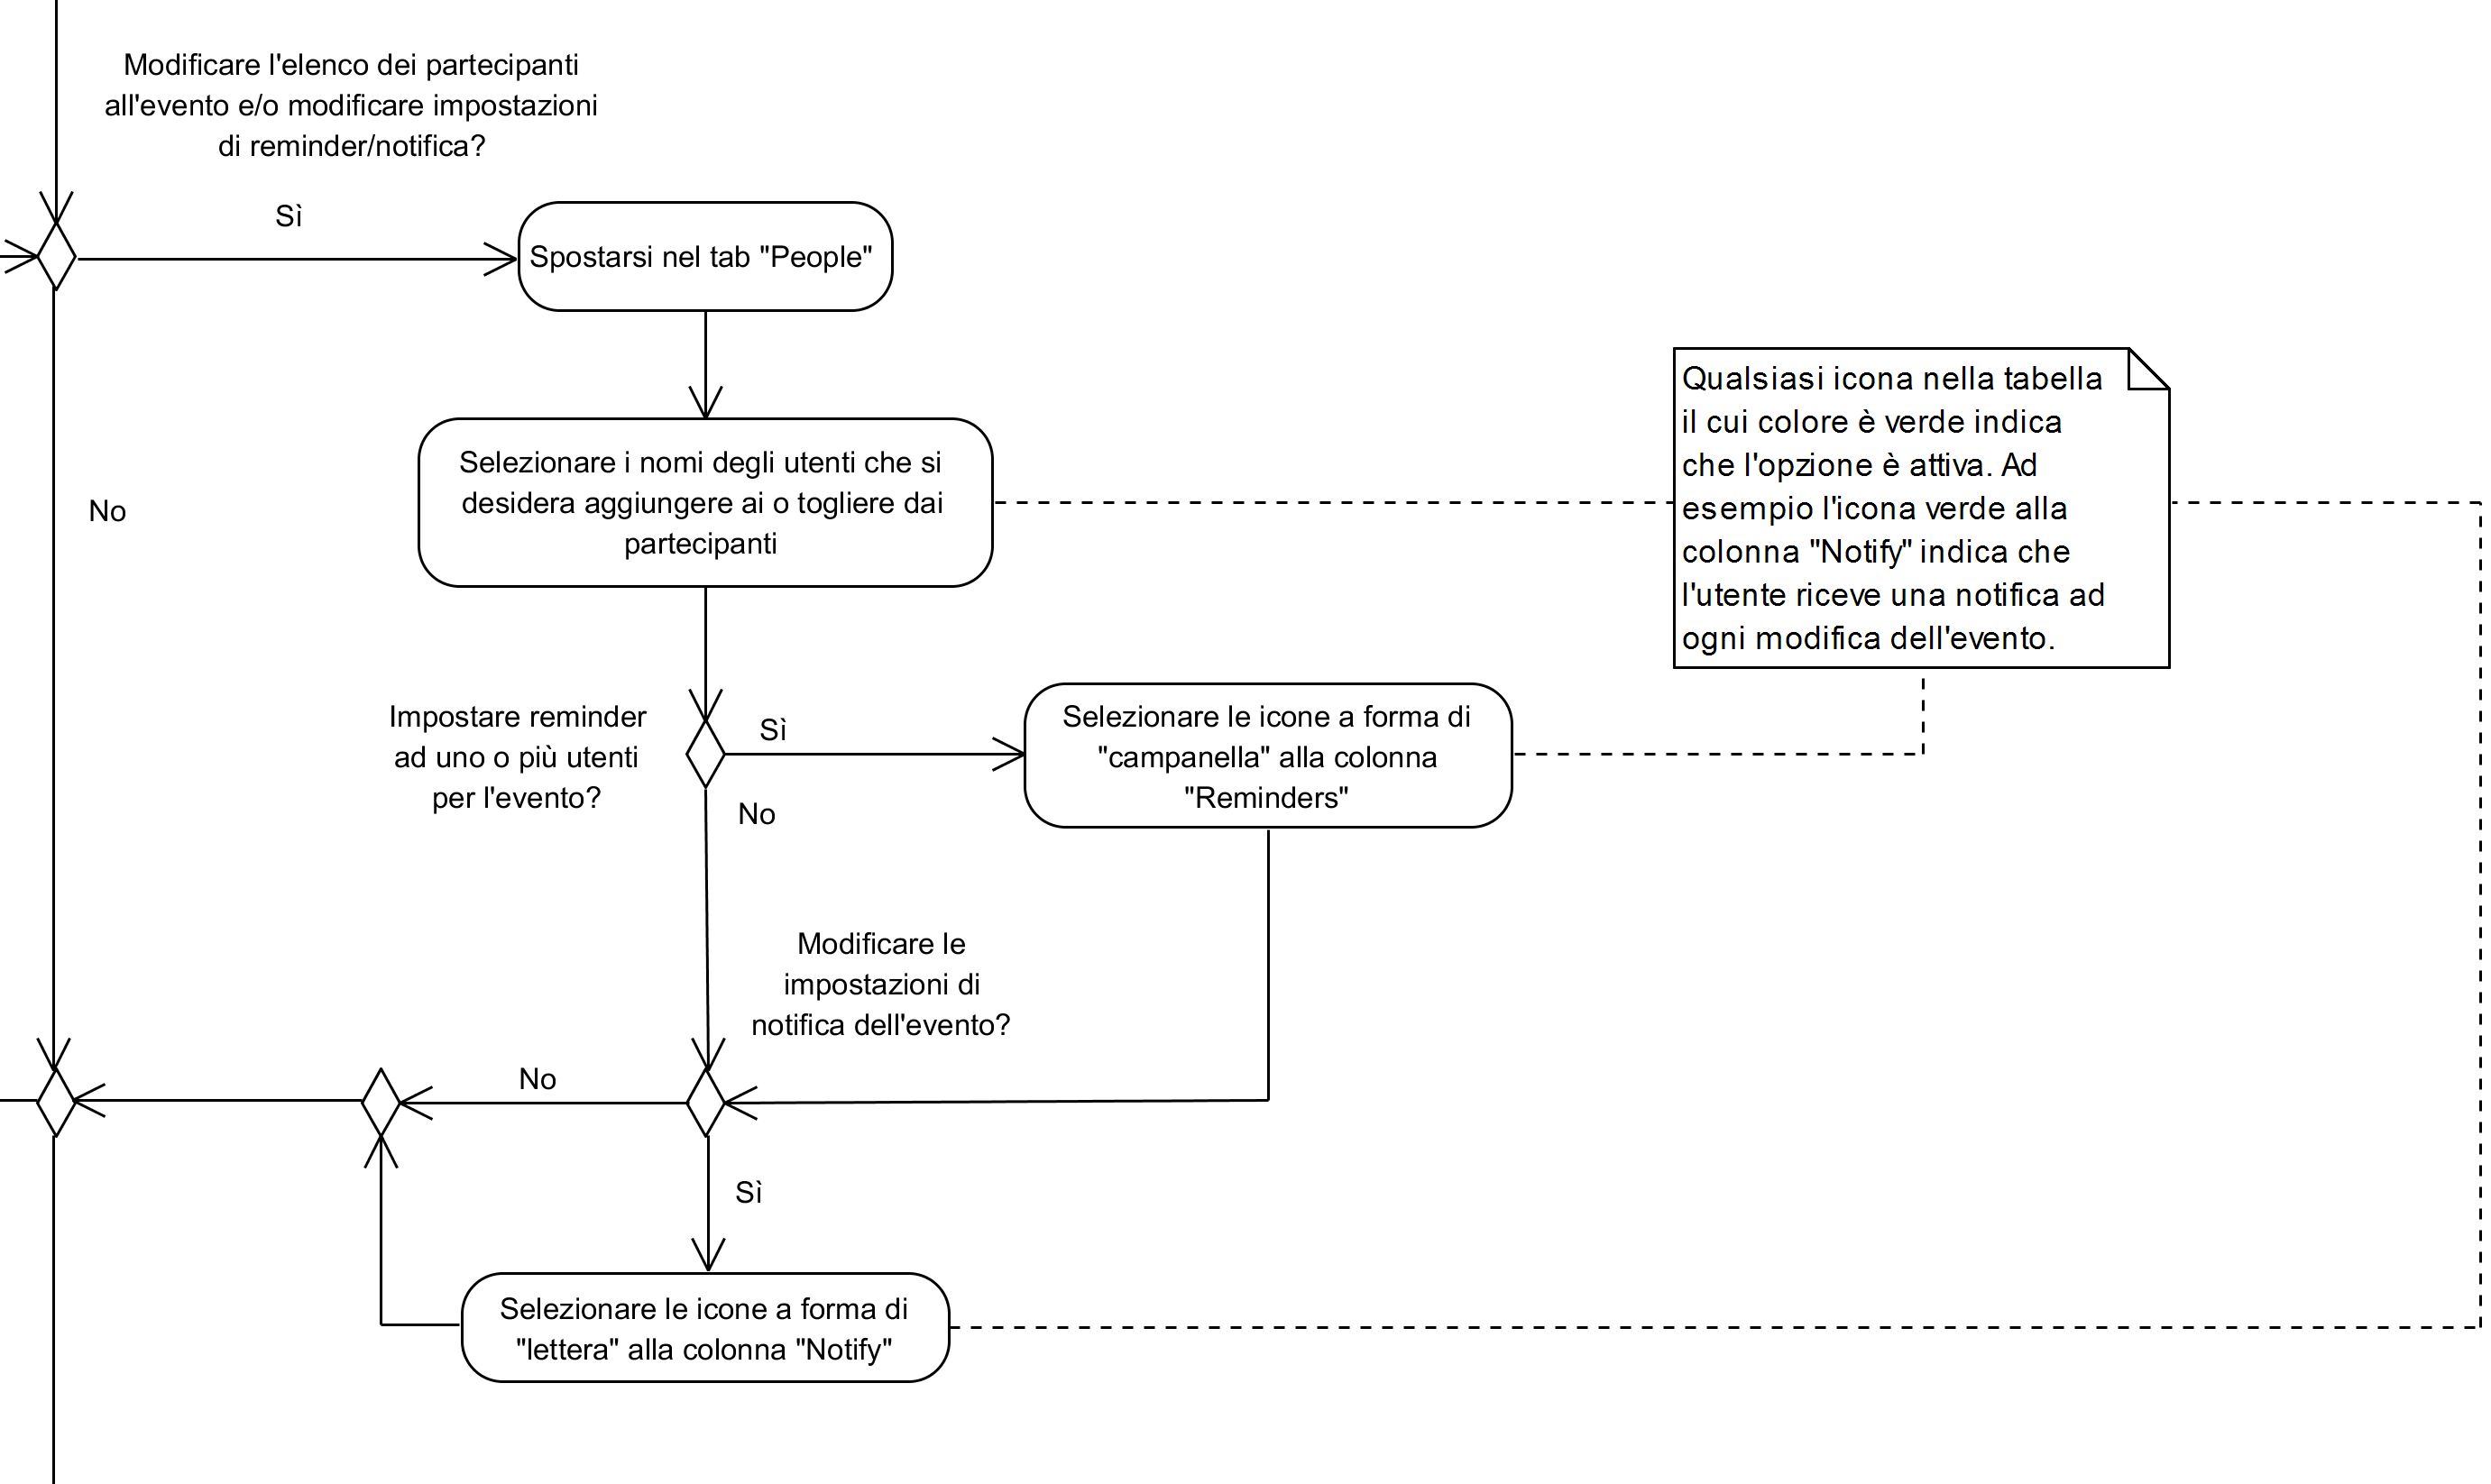
\includegraphics[width=15cm]{../../documenti/NormeDiProgetto/DiagrammiProcedure/EditEventi3.png}
	\captionof{figure}{Procedura di modifica di un evento - Sezione modifica impostazioni dei partecipanti}
\end{center}

\begin{center}
	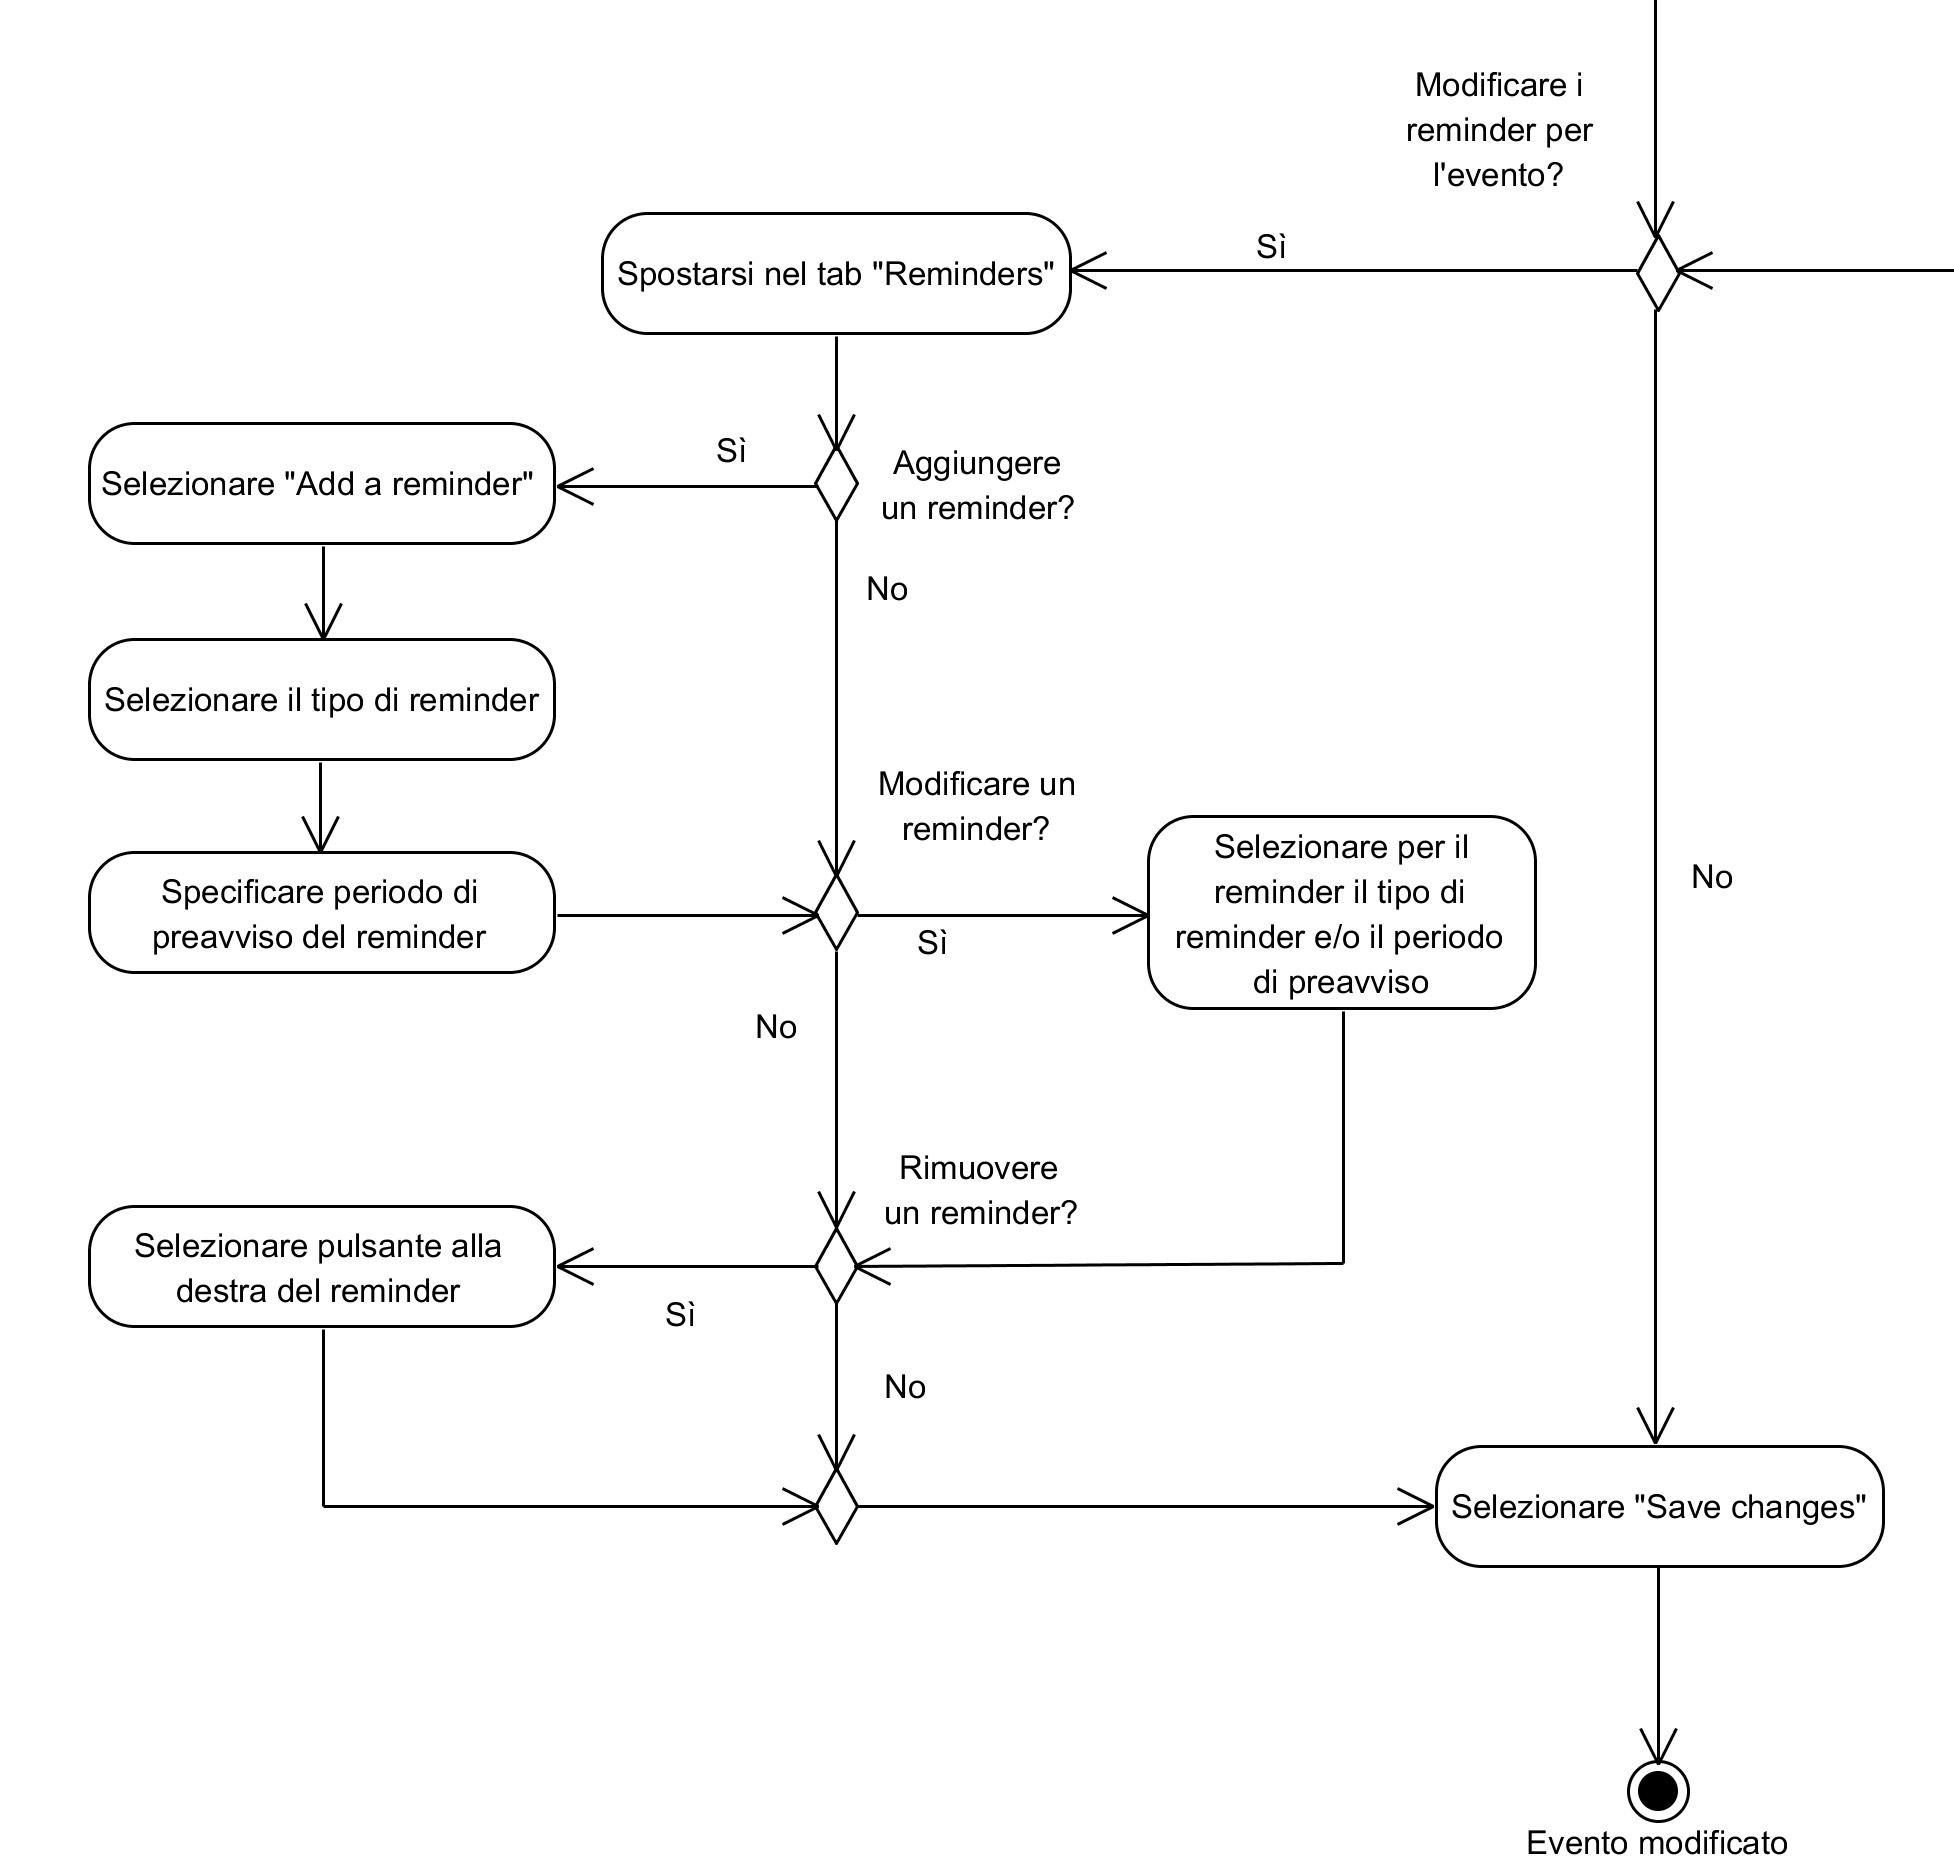
\includegraphics[width=15cm]{../../documenti/NormeDiProgetto/DiagrammiProcedure/EditEventi4.png}
	\captionof{figure}{Procedura di modifica di un evento - Modifica reminder}
\end{center}

\newpage
\paragraph{Procedura di modifica di un Task:}

\begin{center}
	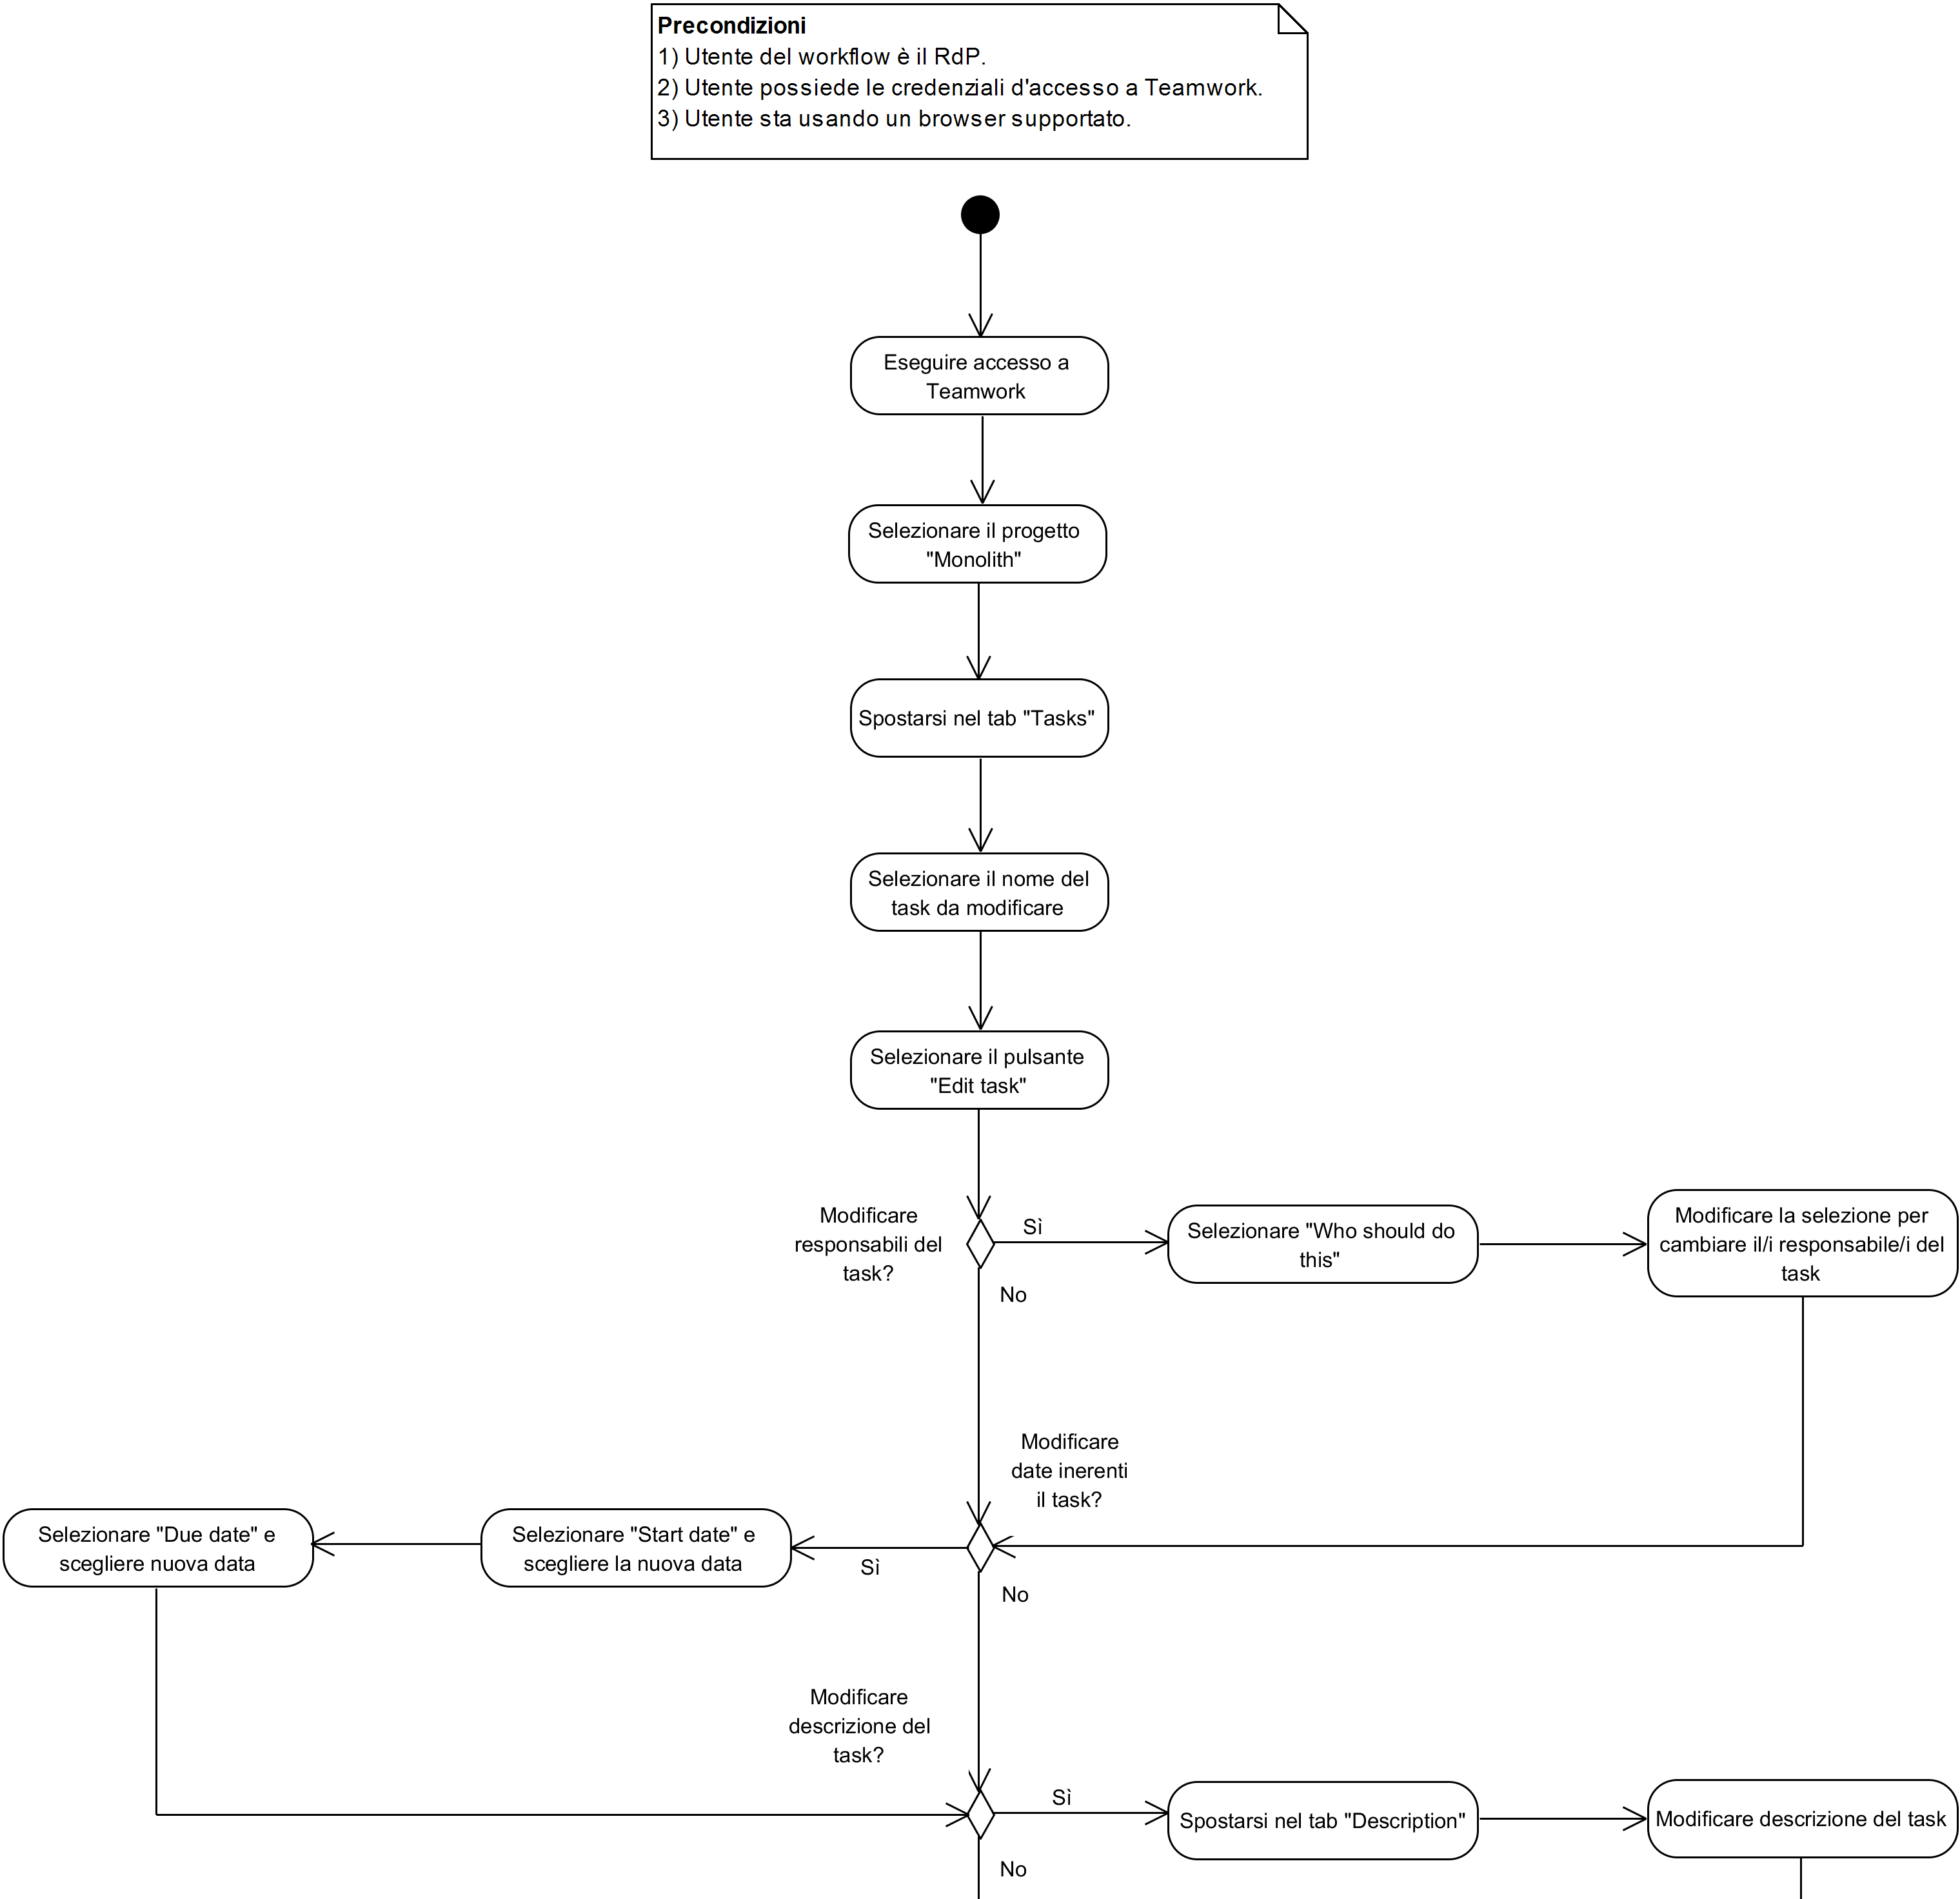
\includegraphics[width=15cm]{../../documenti/NormeDiProgetto/DiagrammiProcedure/EditTask1.png}
	\captionof{figure}{Procedura di modifica di un Task - Inizio }
\end{center}

\begin{center}
	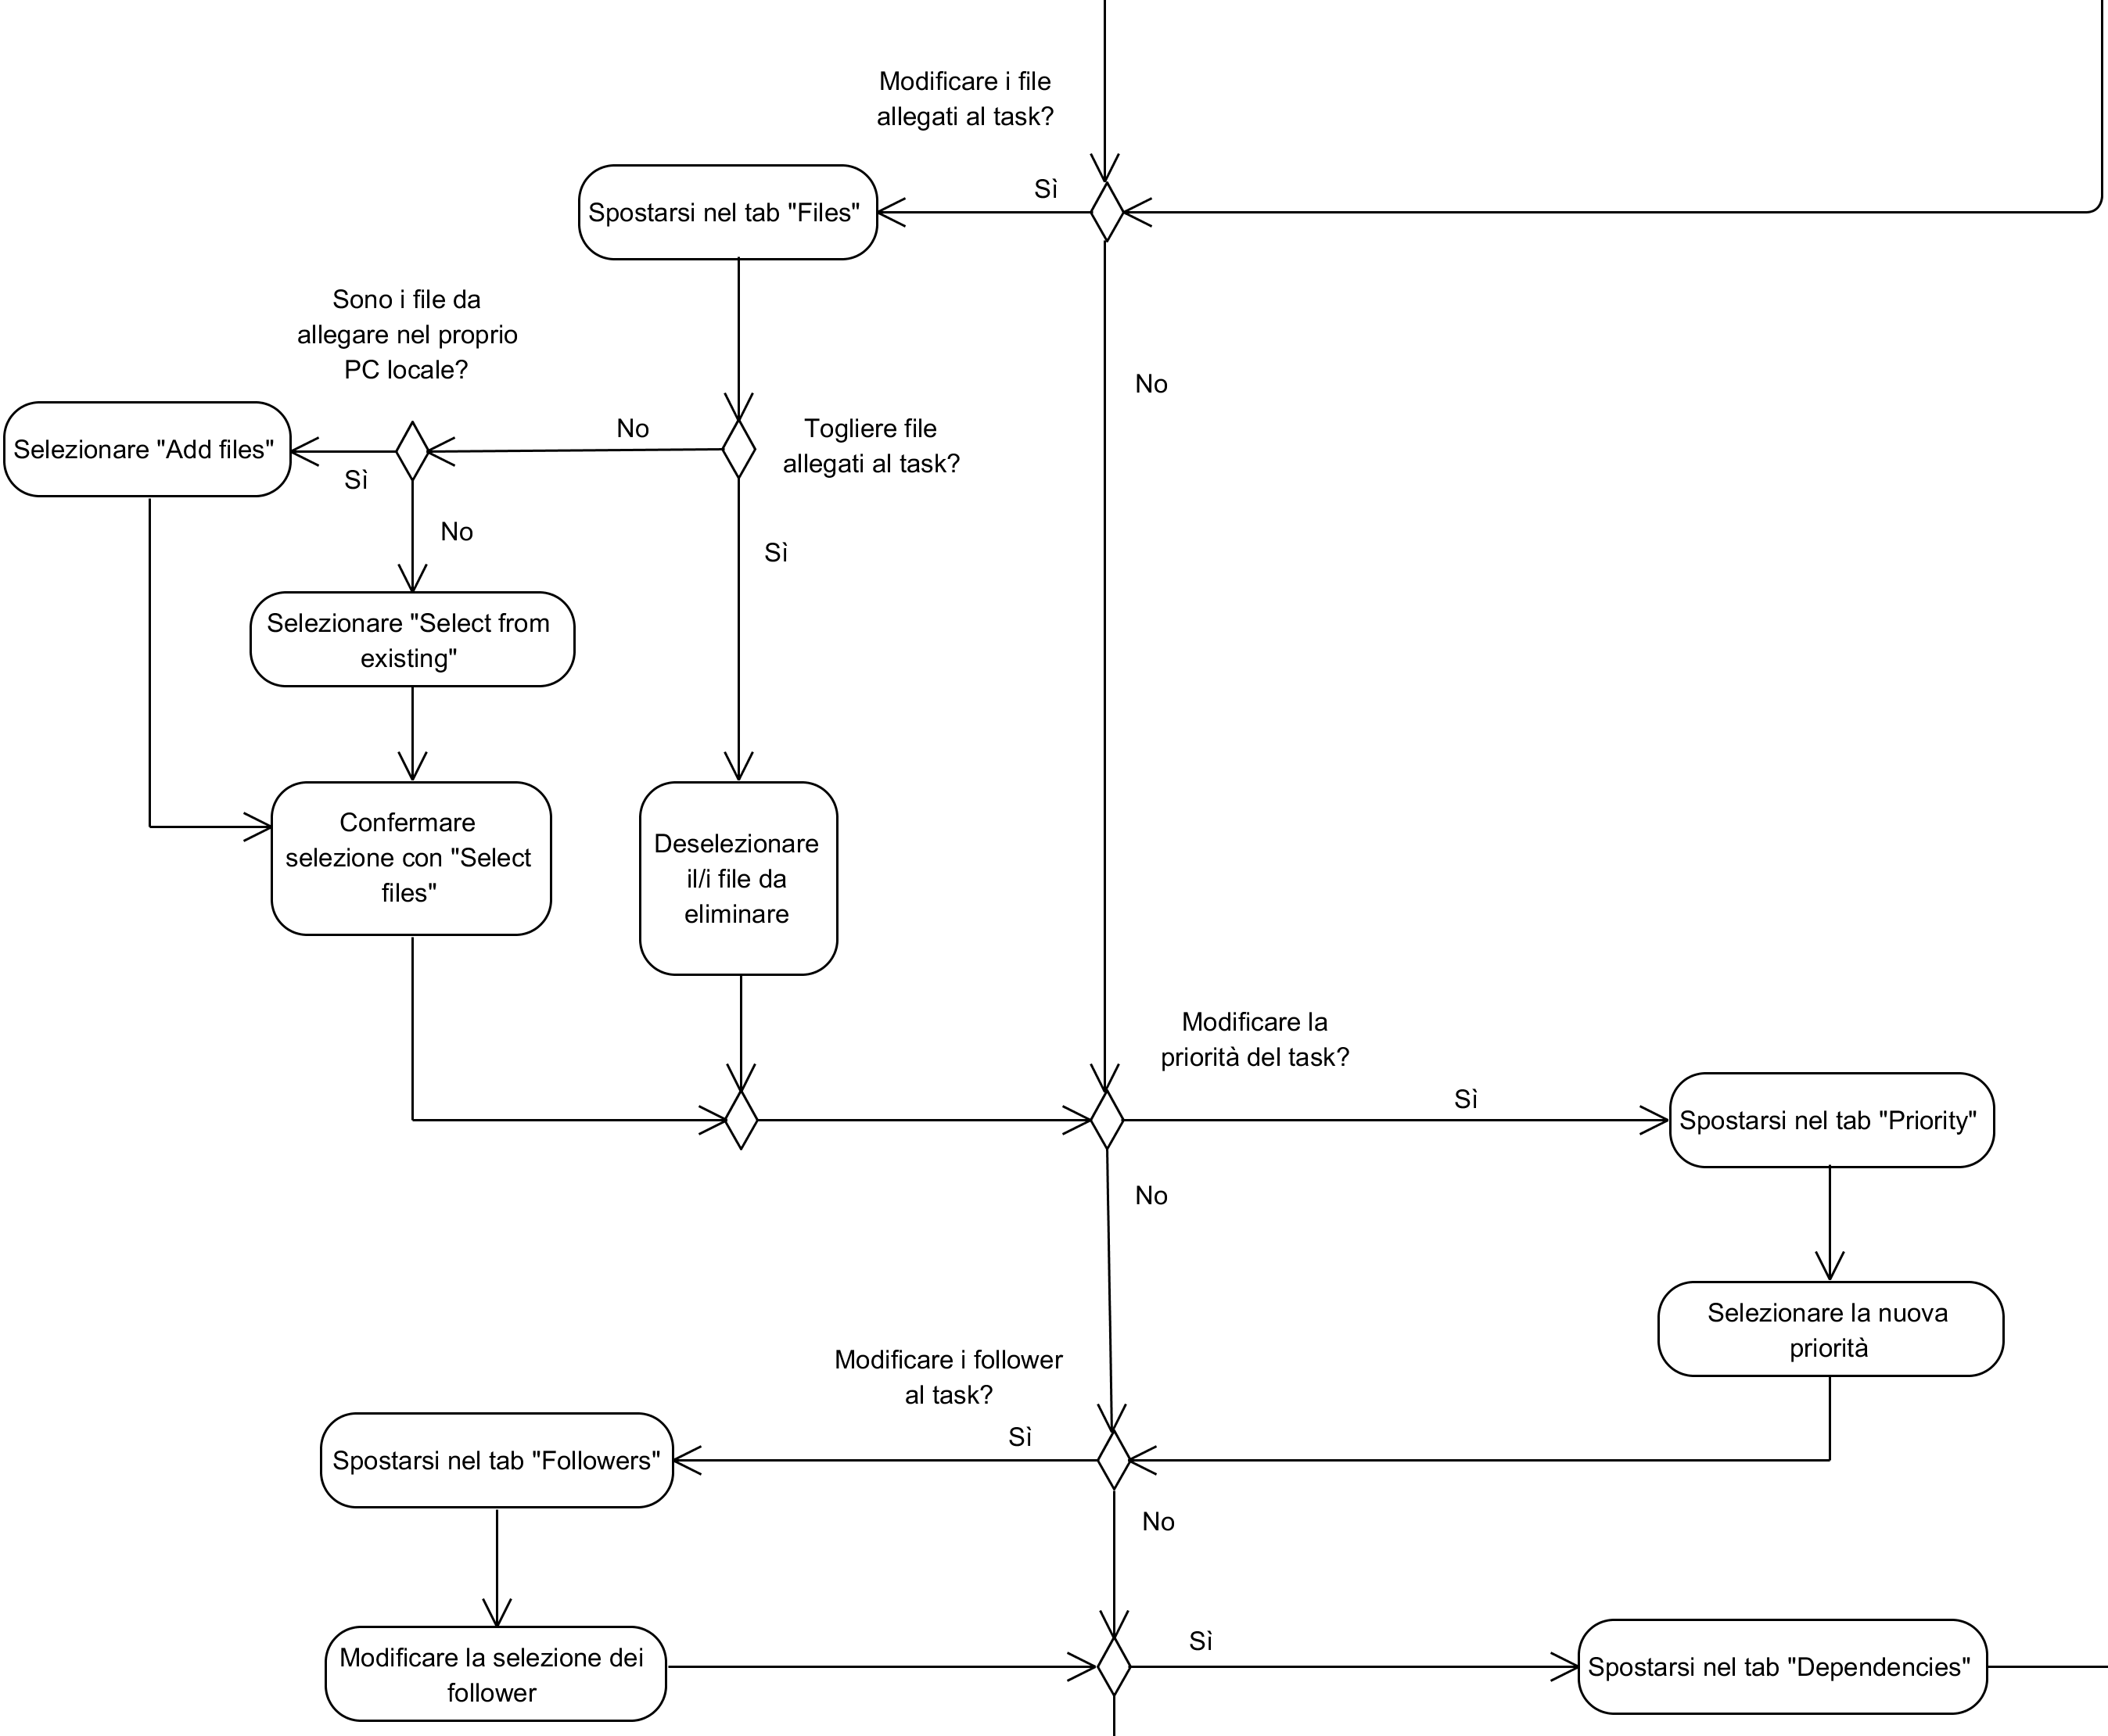
\includegraphics[width=15cm]{../../documenti/NormeDiProgetto/DiagrammiProcedure/EditTask2.png}
	\captionof{figure}{Procedura di modifica di un Task - Modifica allegati, priorità e follower}
\end{center}

\newpage
\begin{center}
	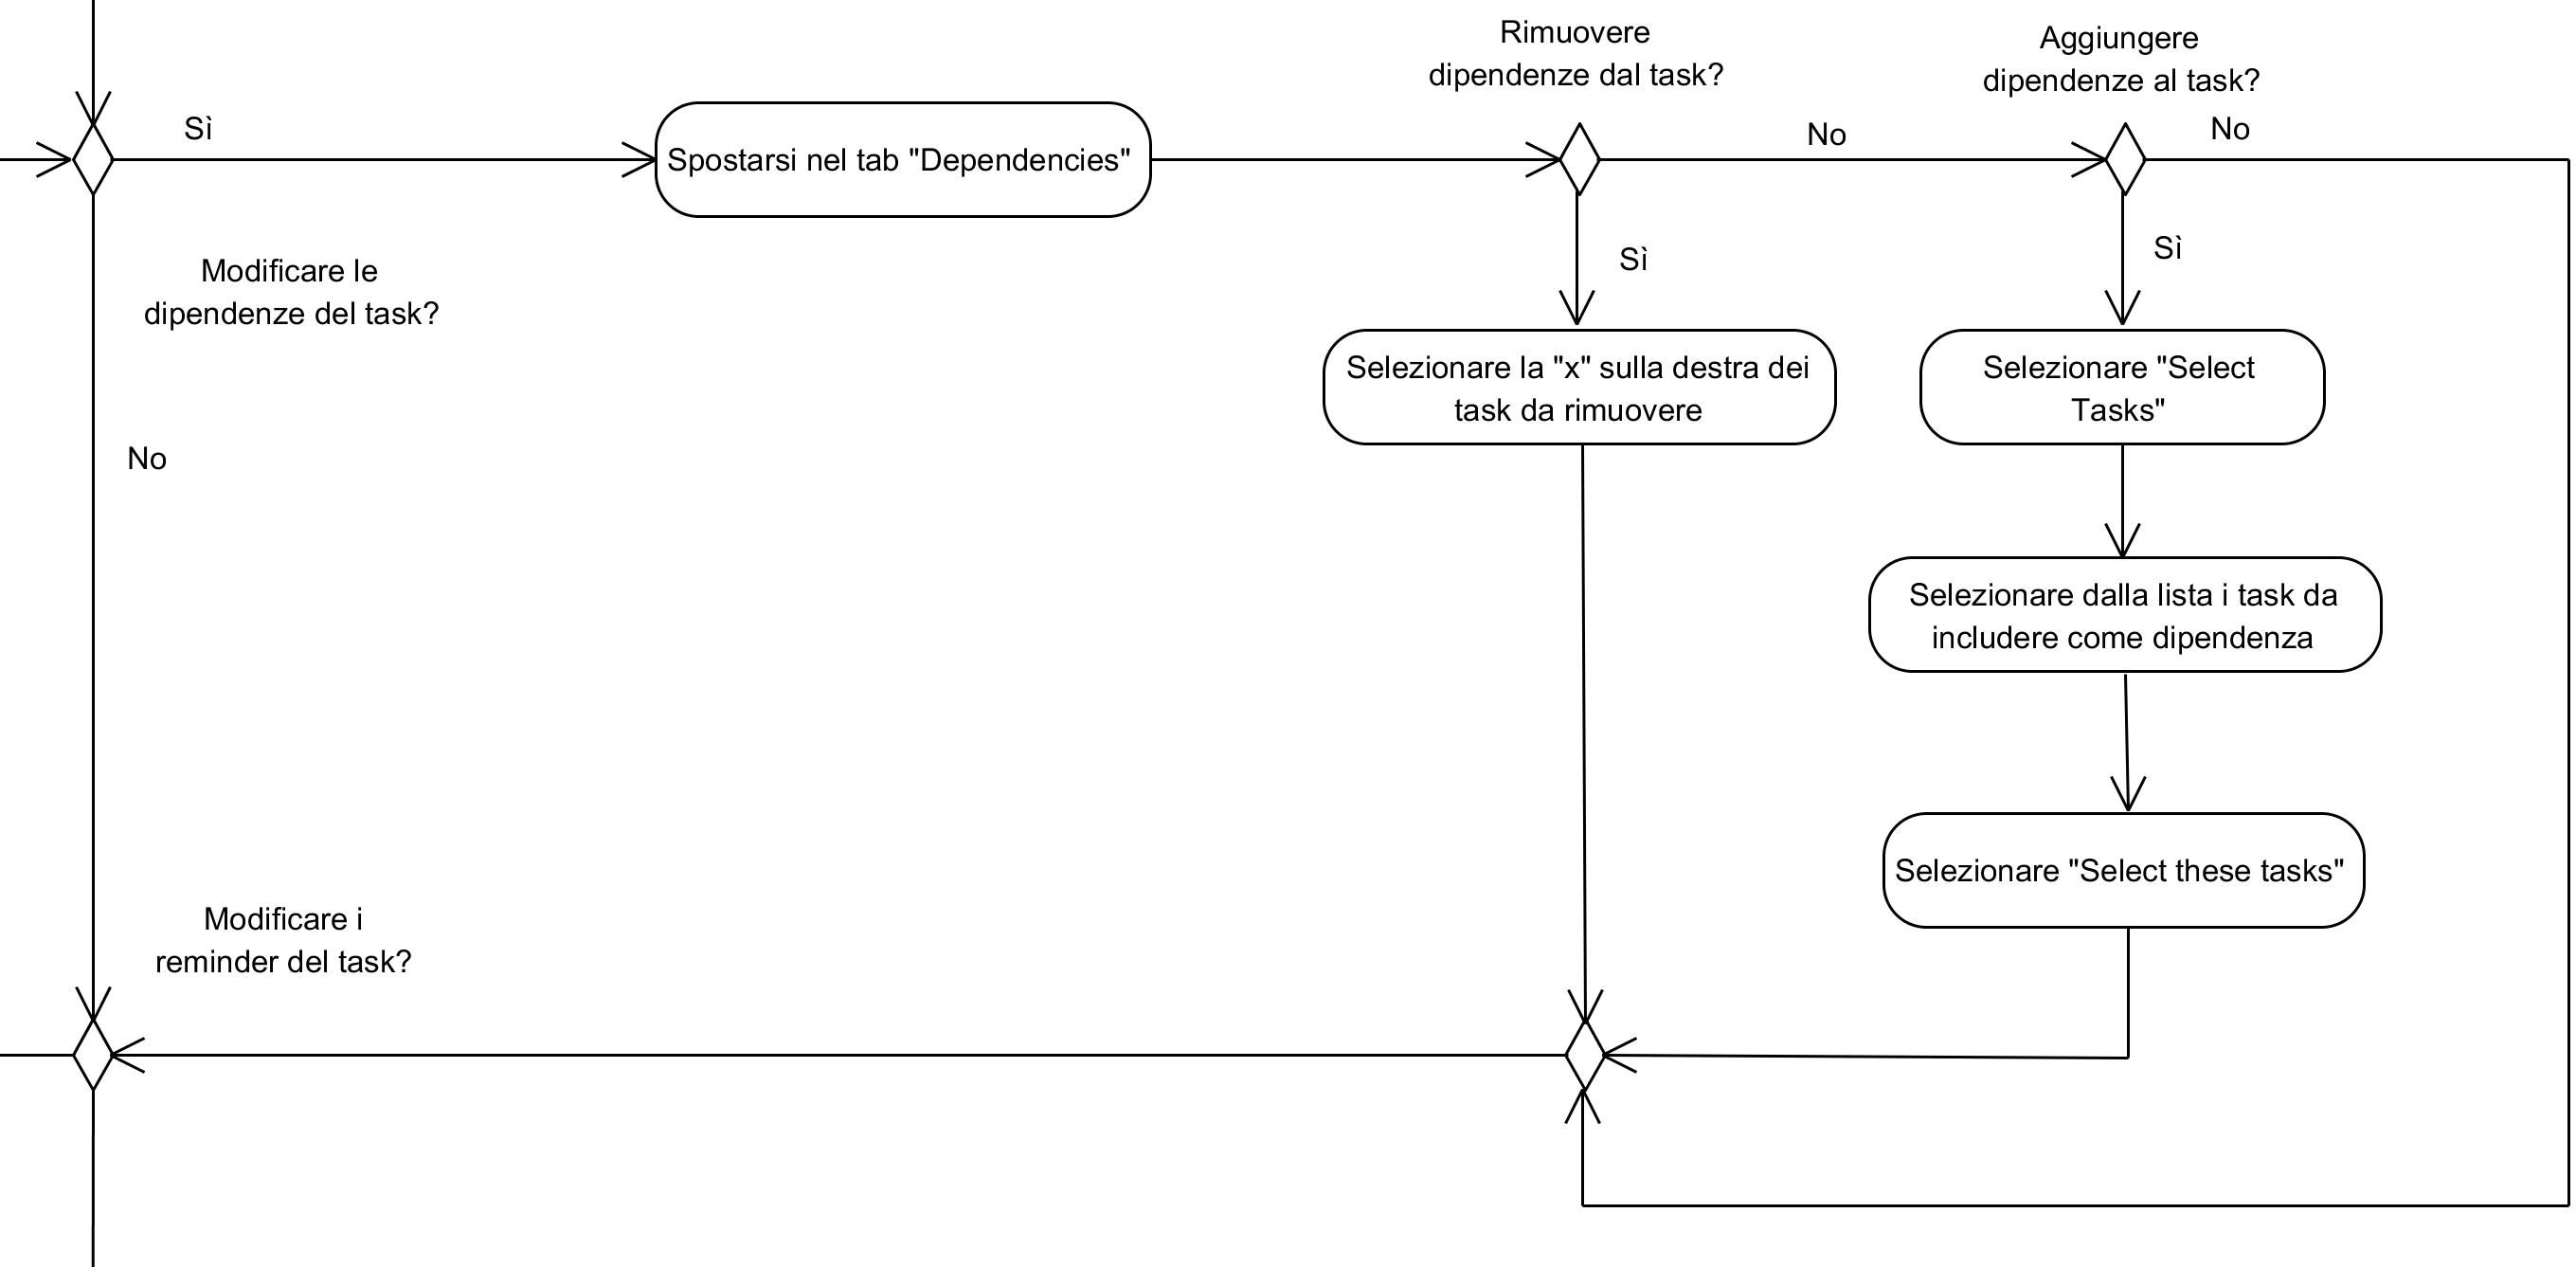
\includegraphics[width=15cm]{../../documenti/NormeDiProgetto/DiagrammiProcedure/EditTask3.png}
	\captionof{figure}{Procedura di modifica di un Task - Modifica dipendenze}
\end{center}

\begin{center}
	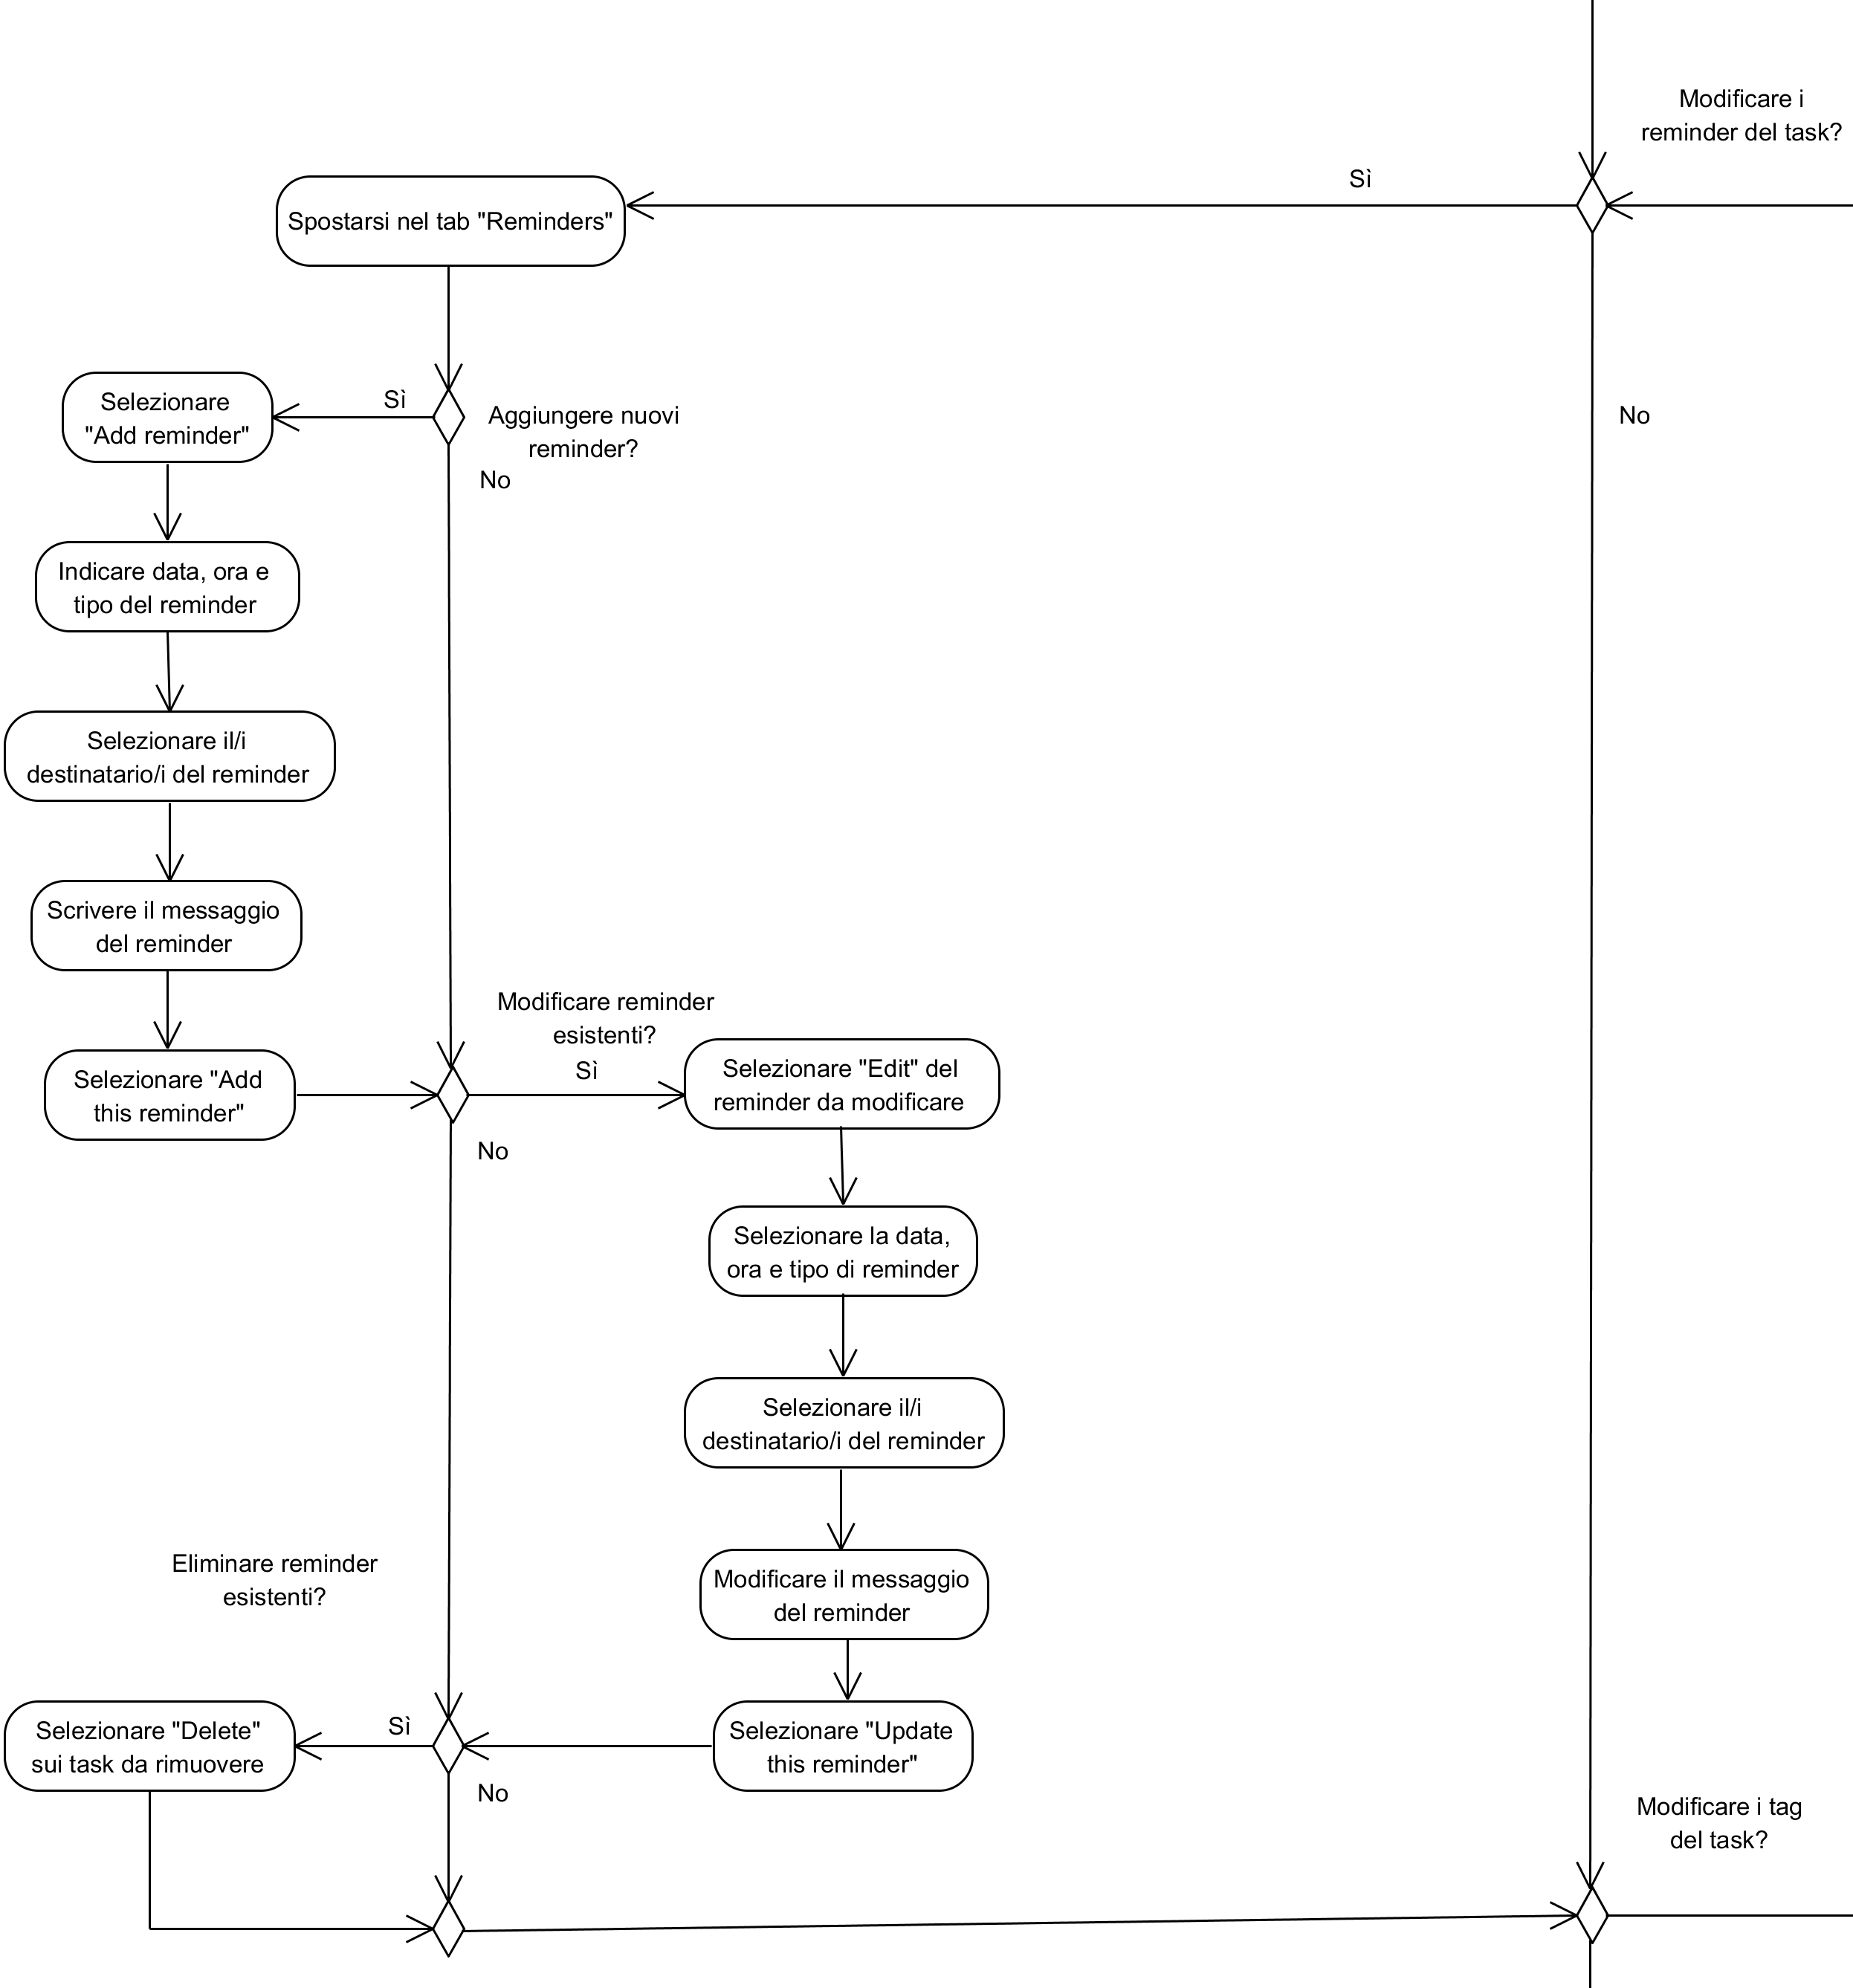
\includegraphics[width=15cm]{../../documenti/NormeDiProgetto/DiagrammiProcedure/EditTask4.png}
	\captionof{figure}{Procedura di modifica di un Task - Modifica reminder}
\end{center}

\begin{center}
	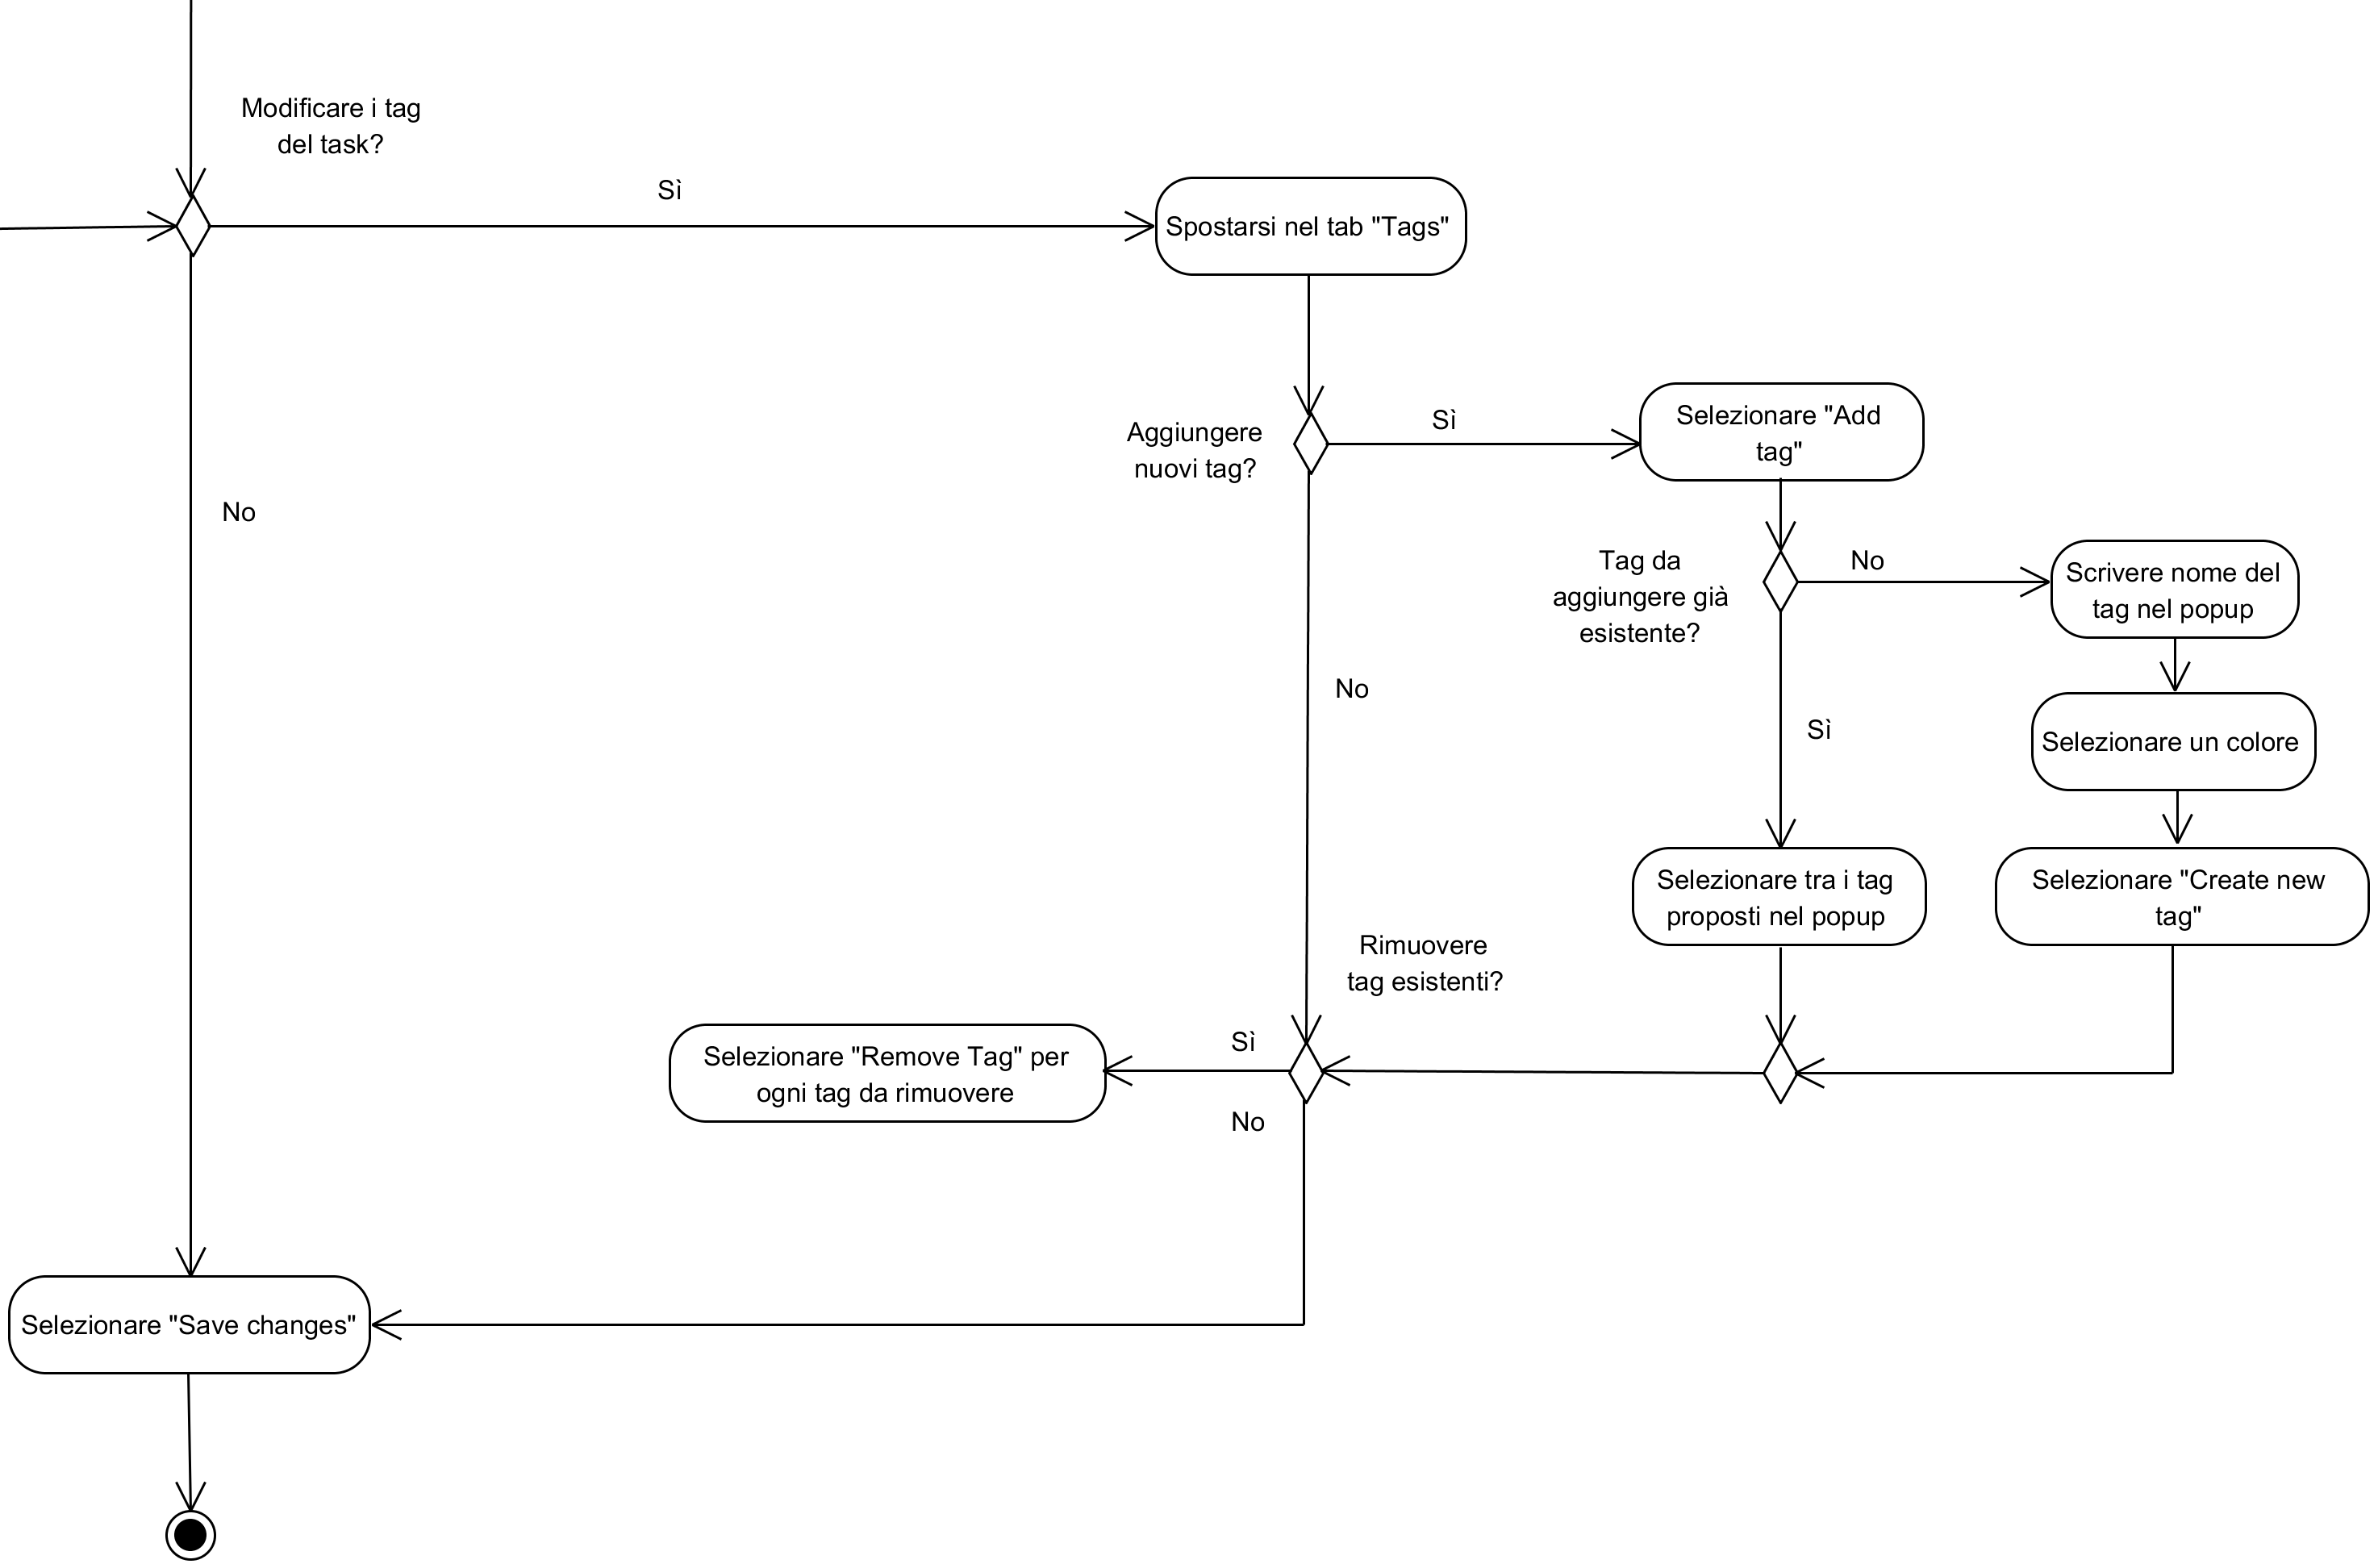
\includegraphics[width=15cm]{../../documenti/NormeDiProgetto/DiagrammiProcedure/EditTask5.png}
	\captionof{figure}{Procedura di modifica di un Task - Modifica tag}
\end{center}

\paragraph{Procedura di creazione di una riunione interna ordinaria:}

\begin{center}
	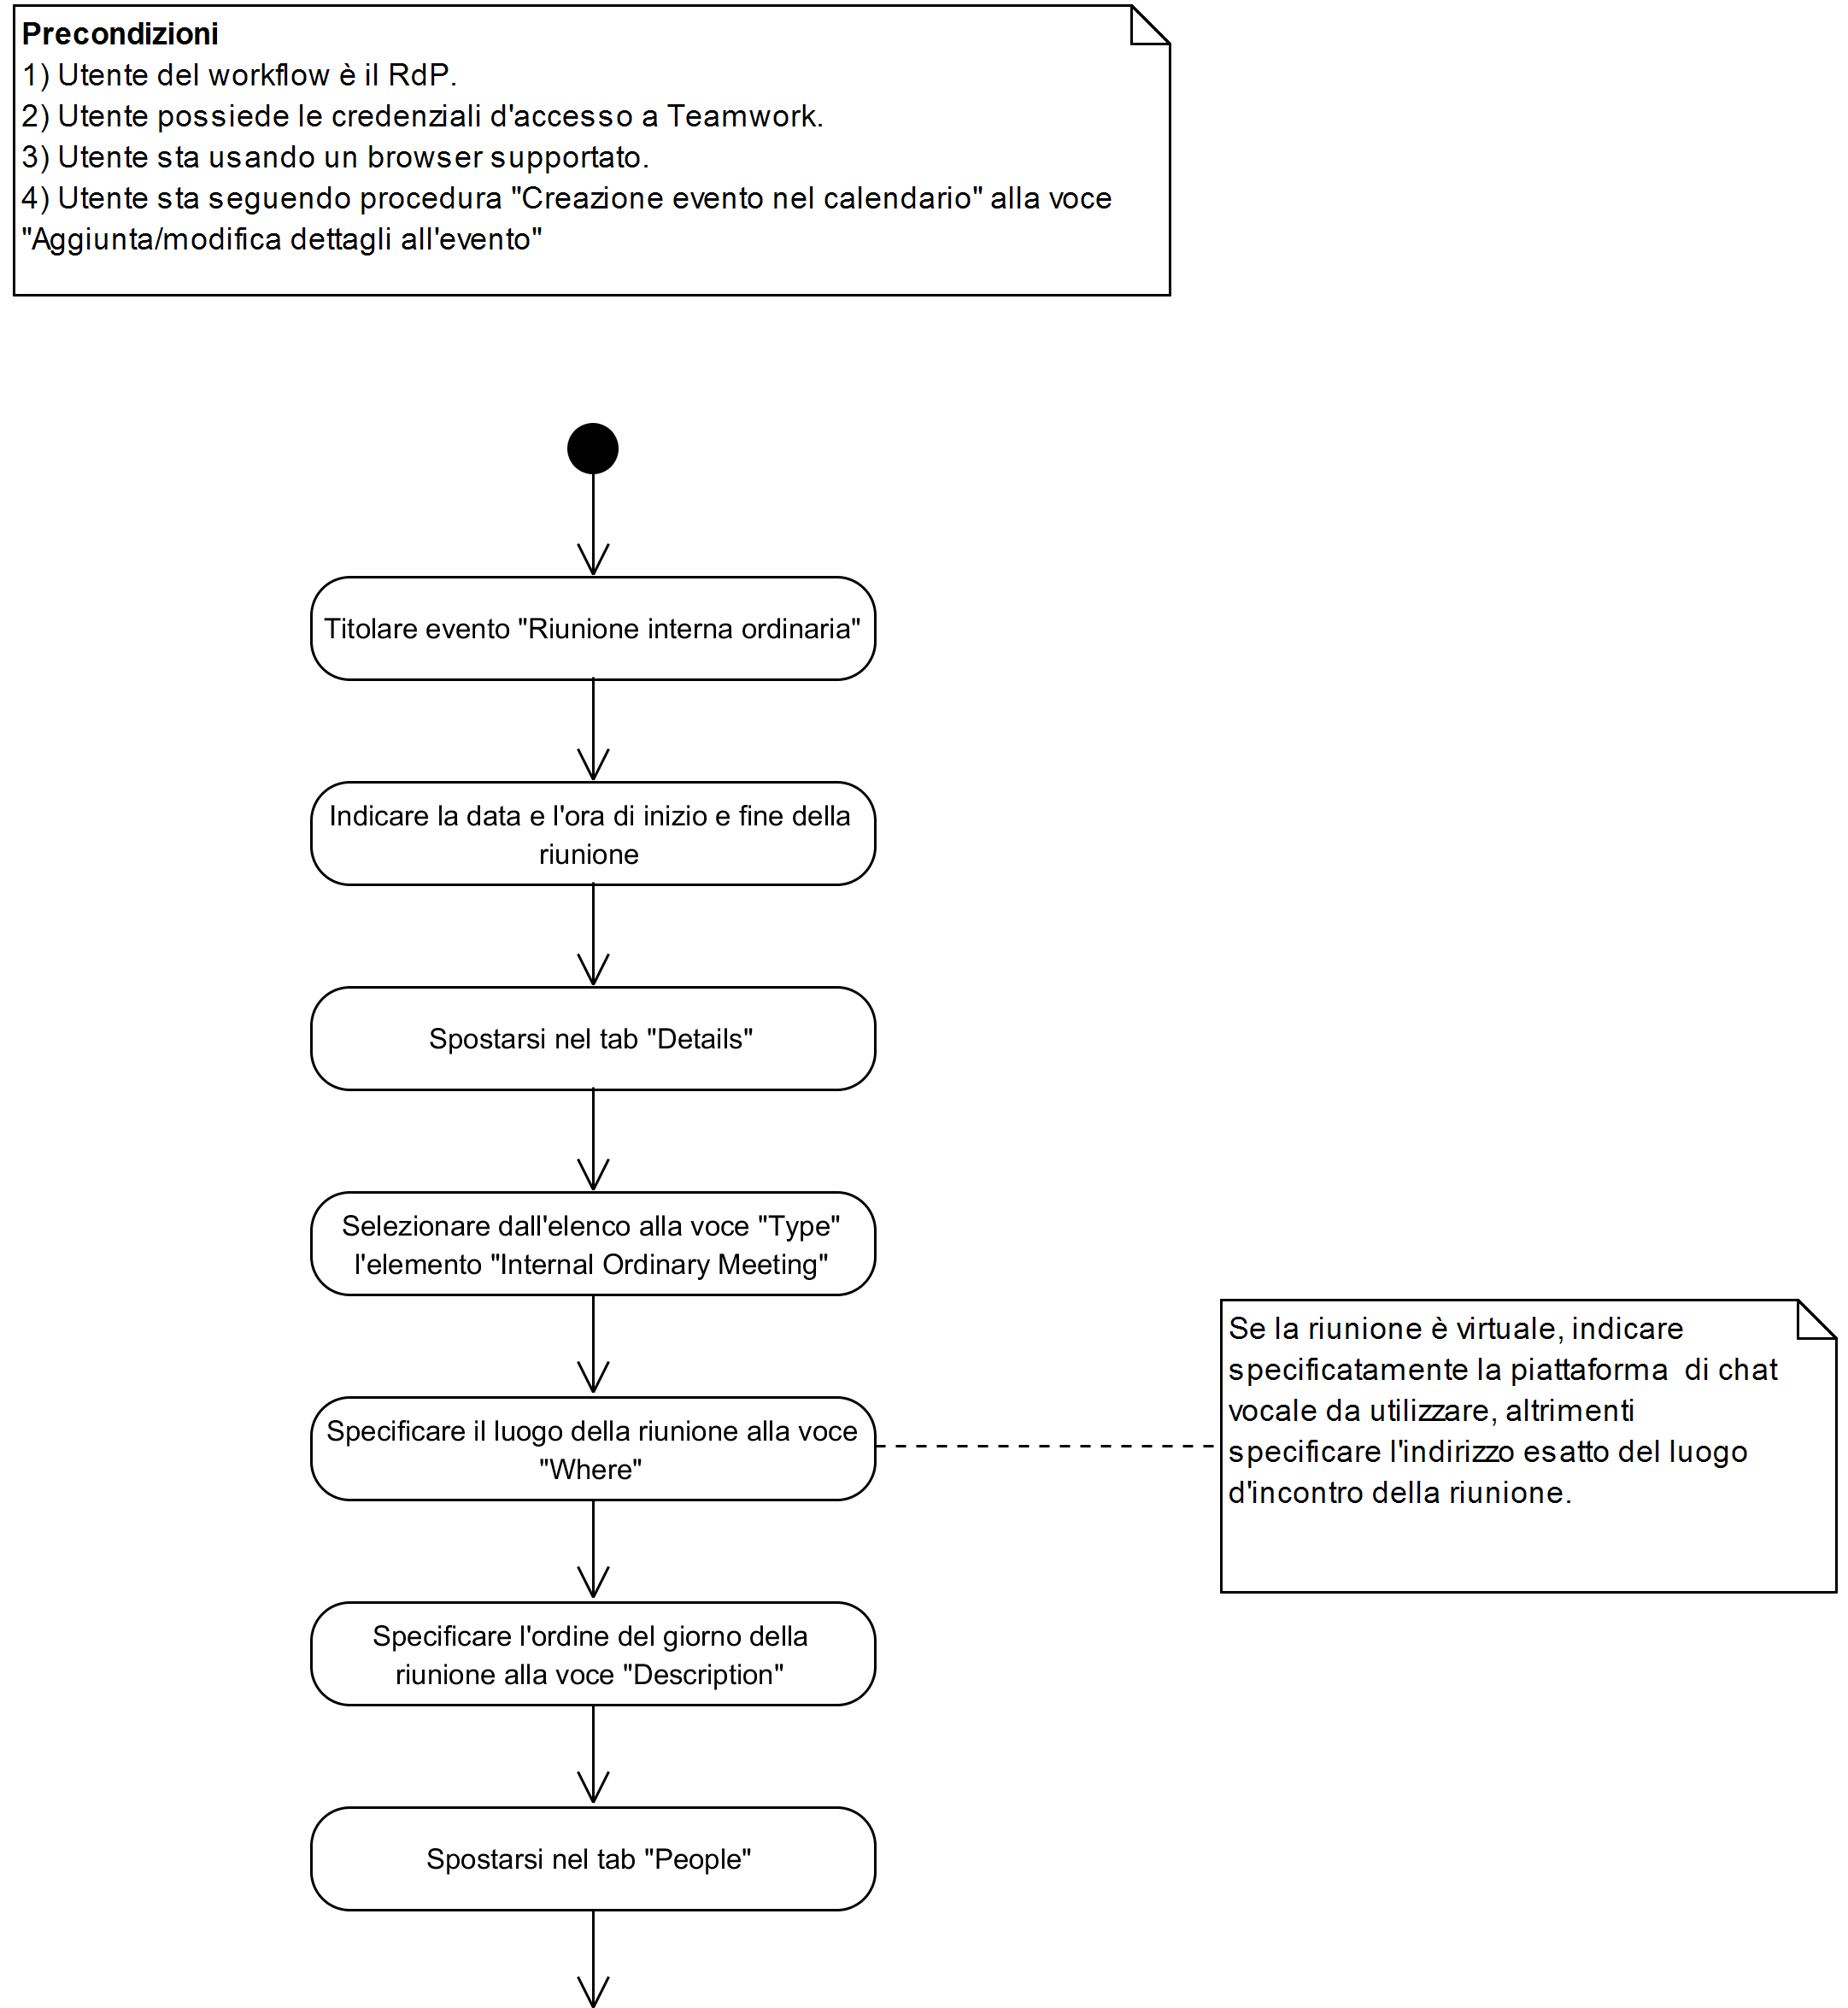
\includegraphics[width=15cm]{../../documenti/NormeDiProgetto/DiagrammiProcedure/RiunioneInternaOrdinaria1.png}
	\captionof{figure}{Procedura di creazione di una riunione interna ordinaria - Parte 1}
\end{center}

\begin{center}
	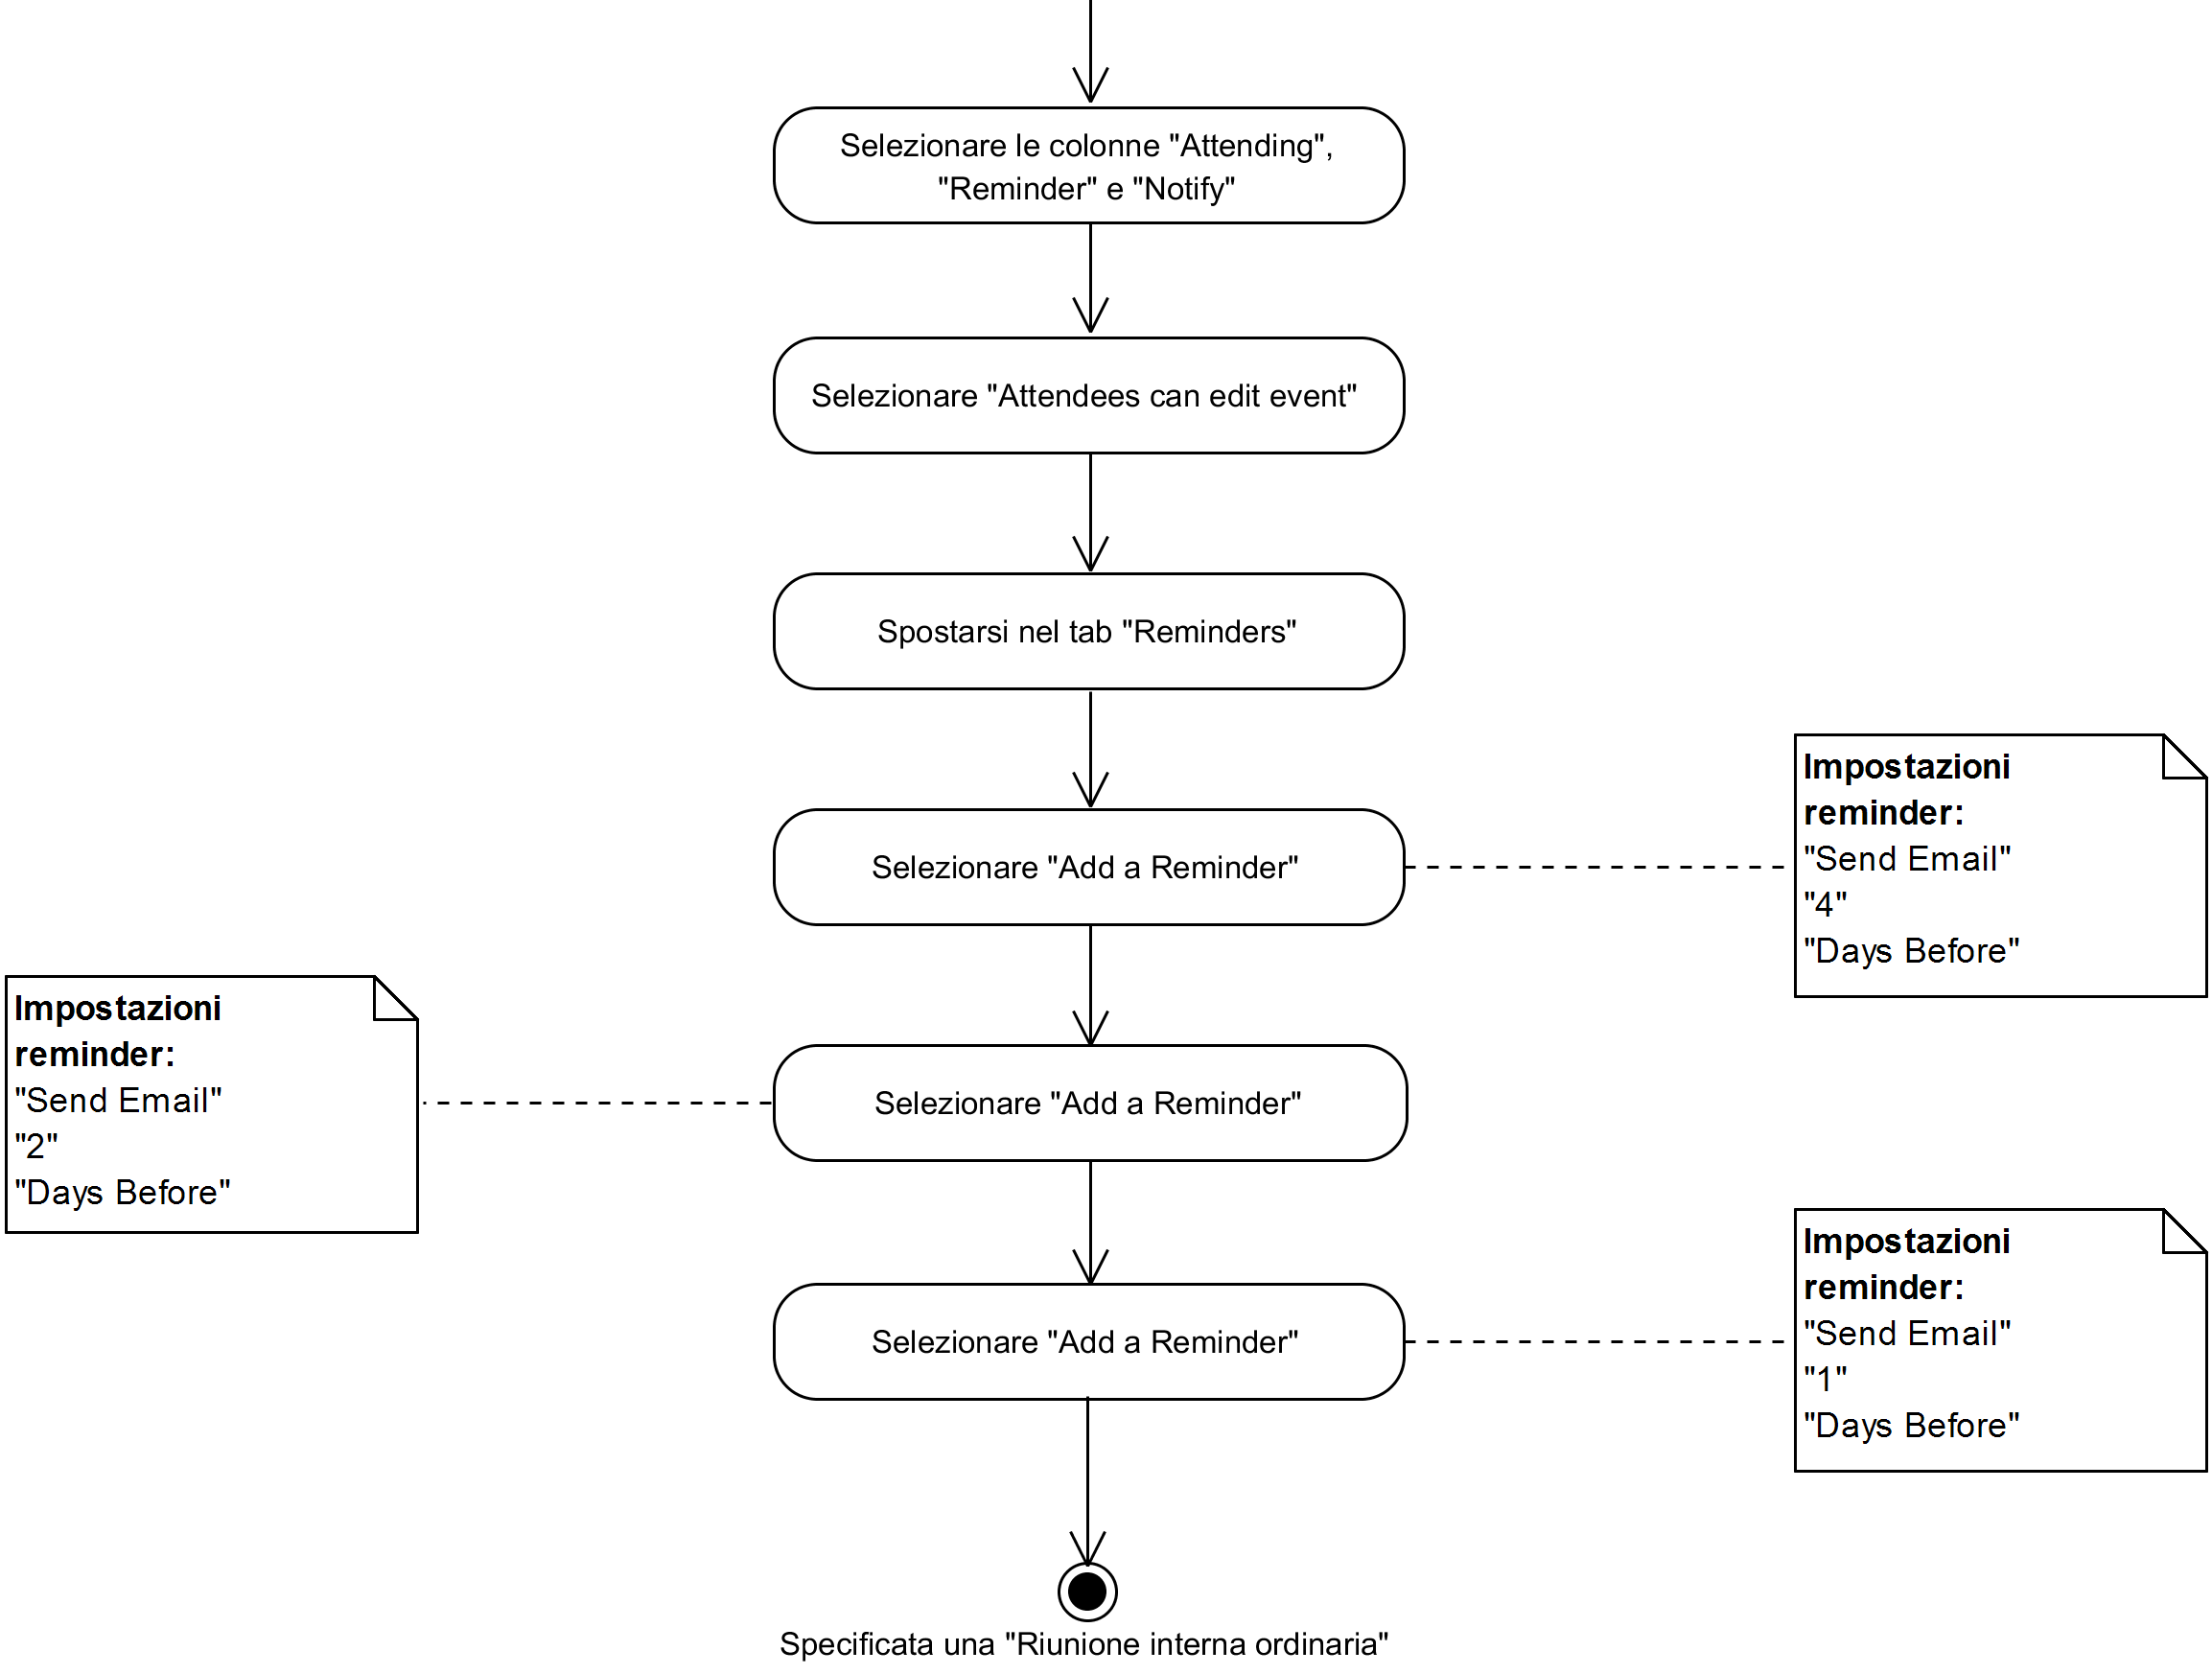
\includegraphics[width=15cm]{../../documenti/NormeDiProgetto/DiagrammiProcedure/RiunioneInternaOrdinaria2.png}
	\captionof{figure}{Procedura di creazione di una riunione interna ordinaria - Parte 2}
\end{center}

\paragraph{Procedura di creazione di una riunione interna di emergenza:}

\begin{center}
	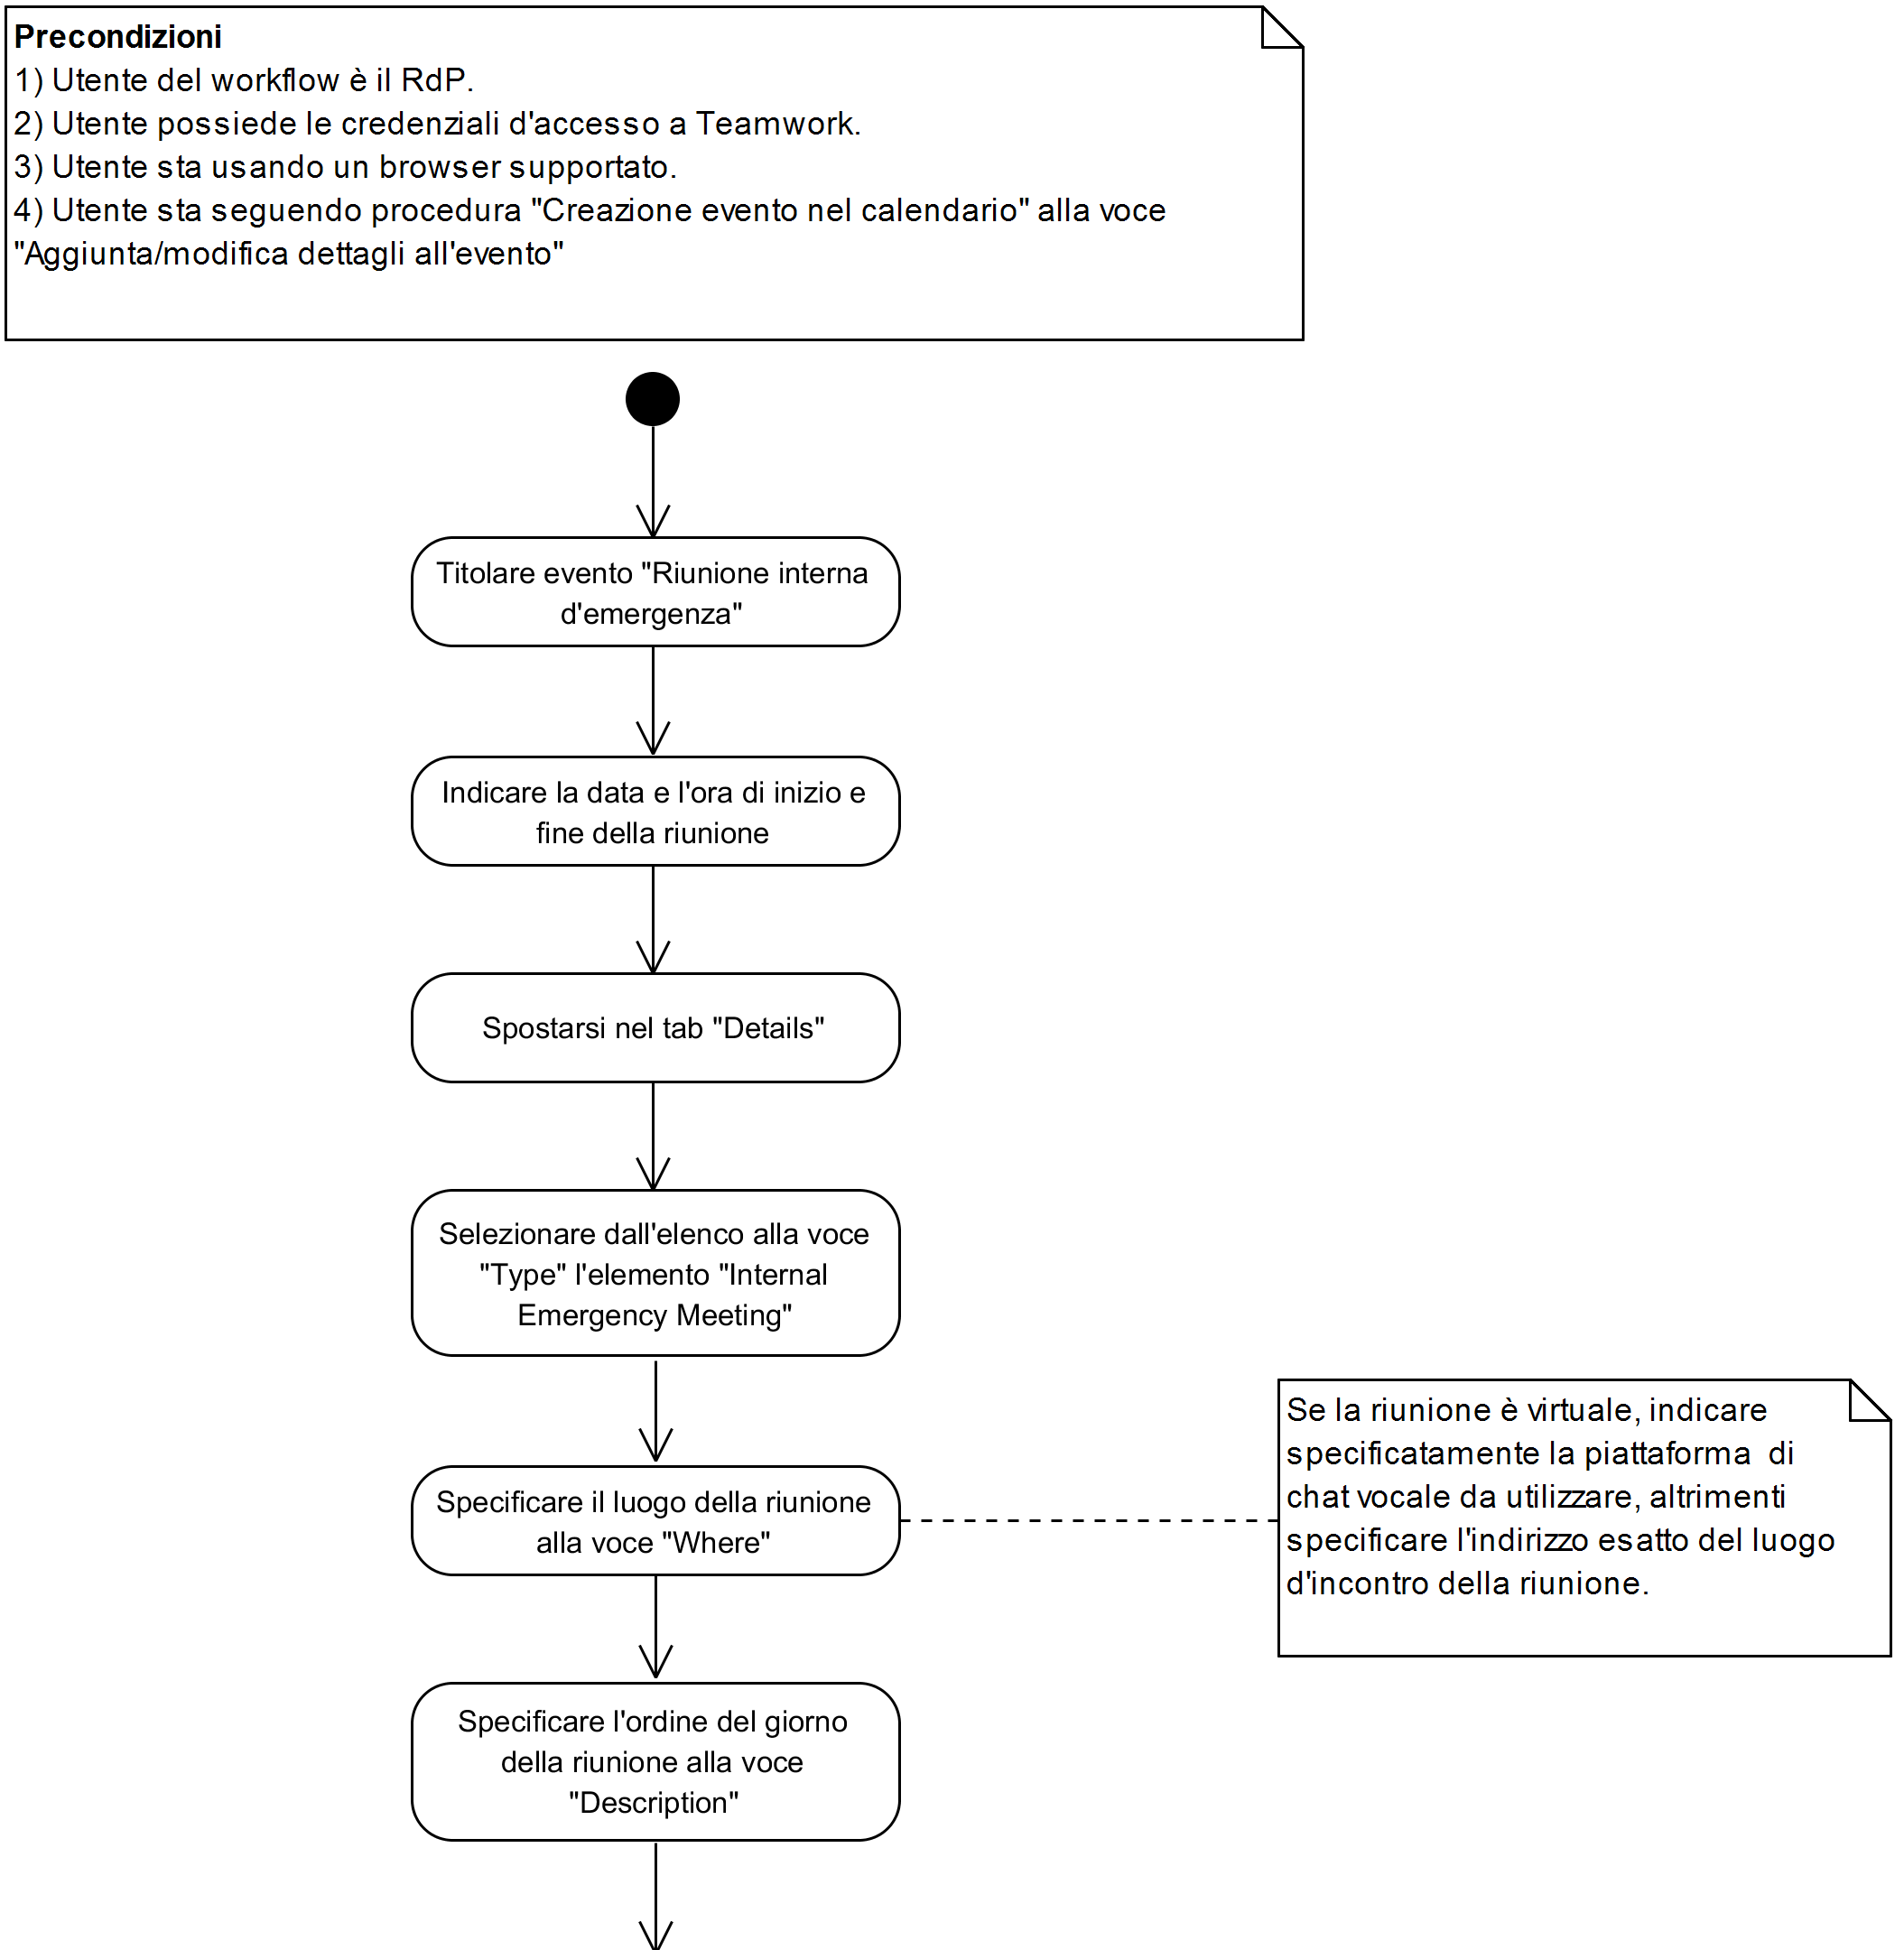
\includegraphics[width=15cm]{../../documenti/NormeDiProgetto/DiagrammiProcedure/RiunioneInternaDiEmergenza1.png}
	\captionof{figure}{Procedura di creazione di una riunione interna di emergenza - Parte 1}
\end{center}

\begin{center}
	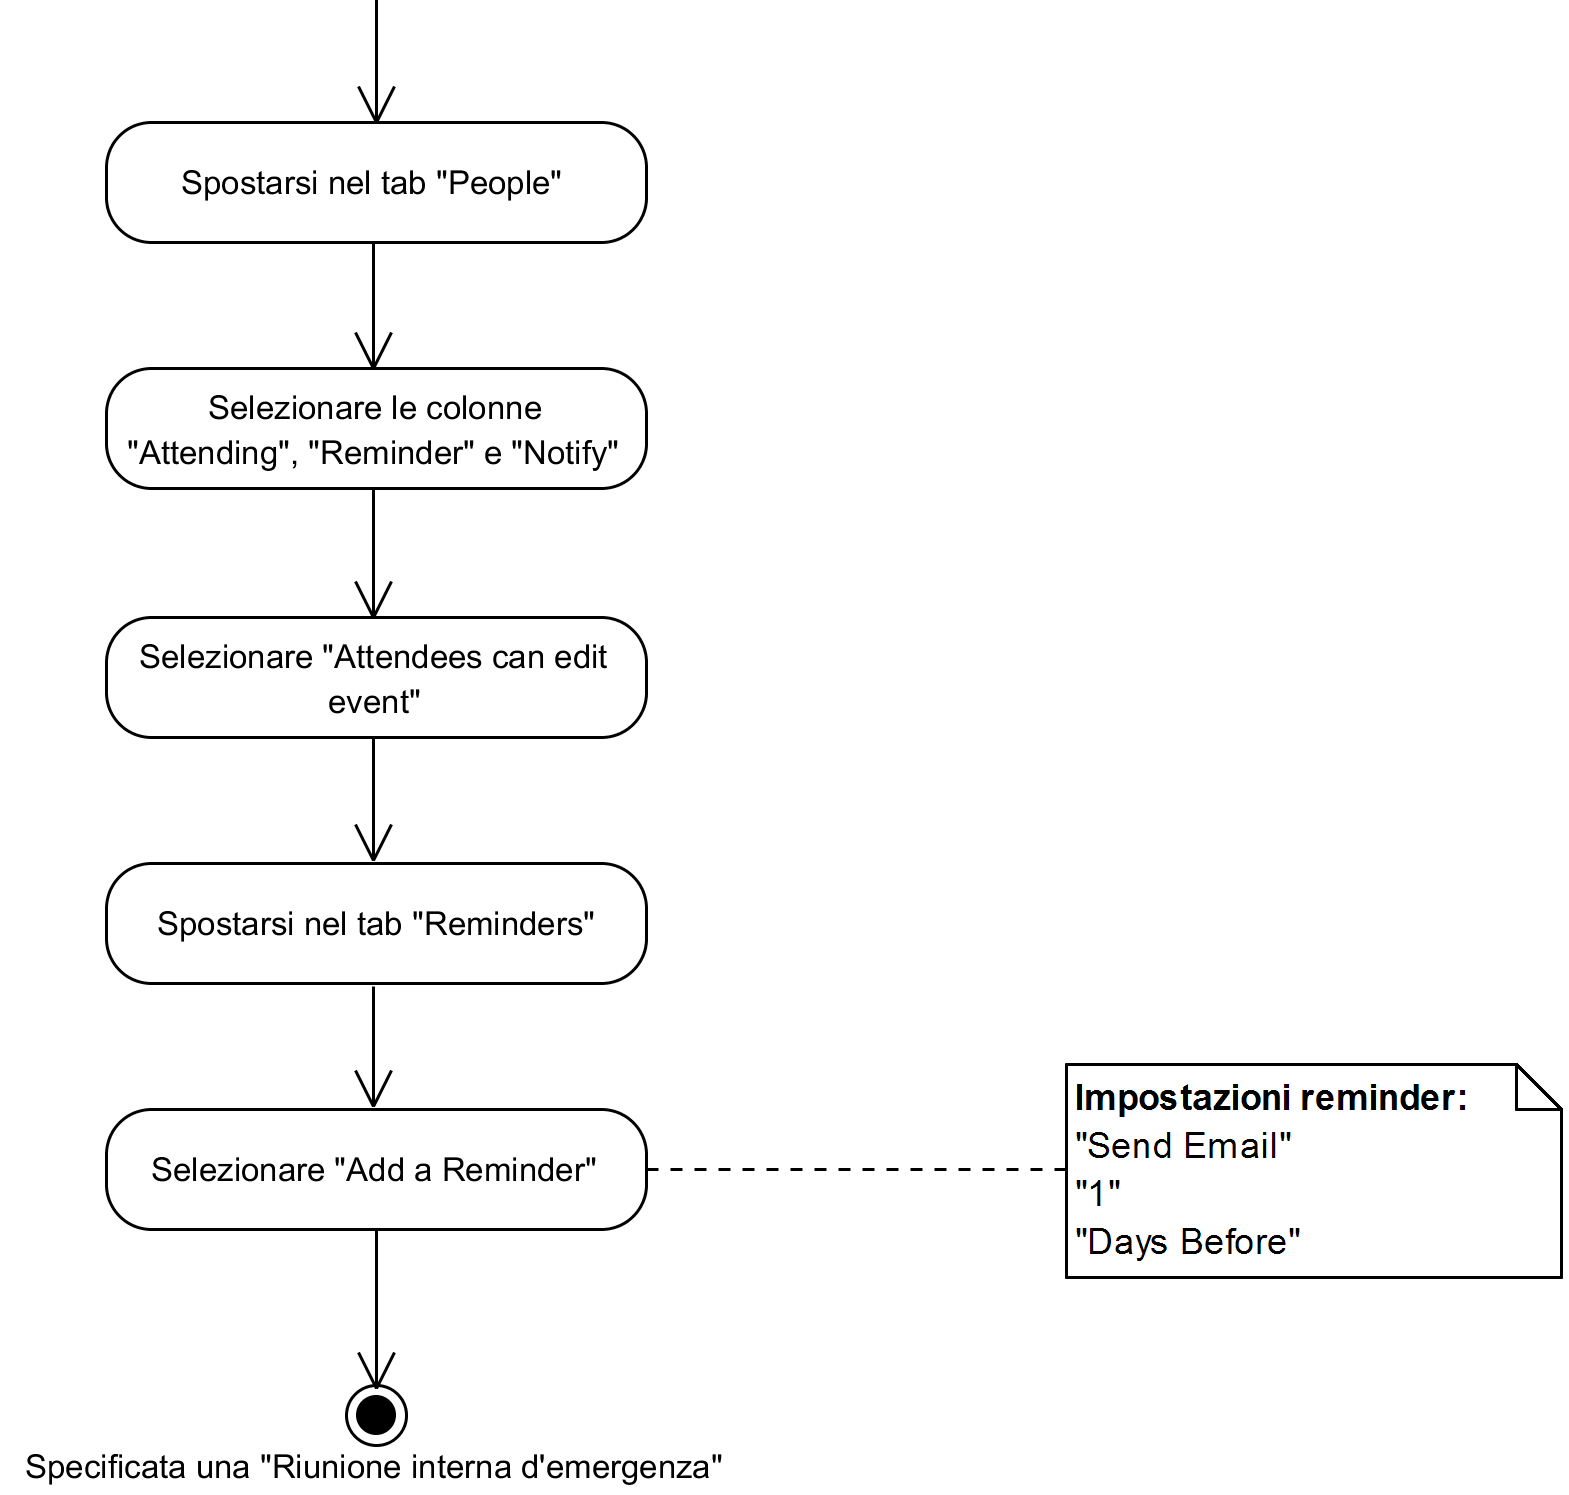
\includegraphics[width=15cm]{../../documenti/NormeDiProgetto/DiagrammiProcedure/RiunioneInternaDiEmergenza2.png}
	\captionof{figure}{Procedura di creazione di una riunione interna di emergenza - Parte 2}
\end{center}

\paragraph{Procedura di creazione di una riunione esterna:}

\begin{center}
	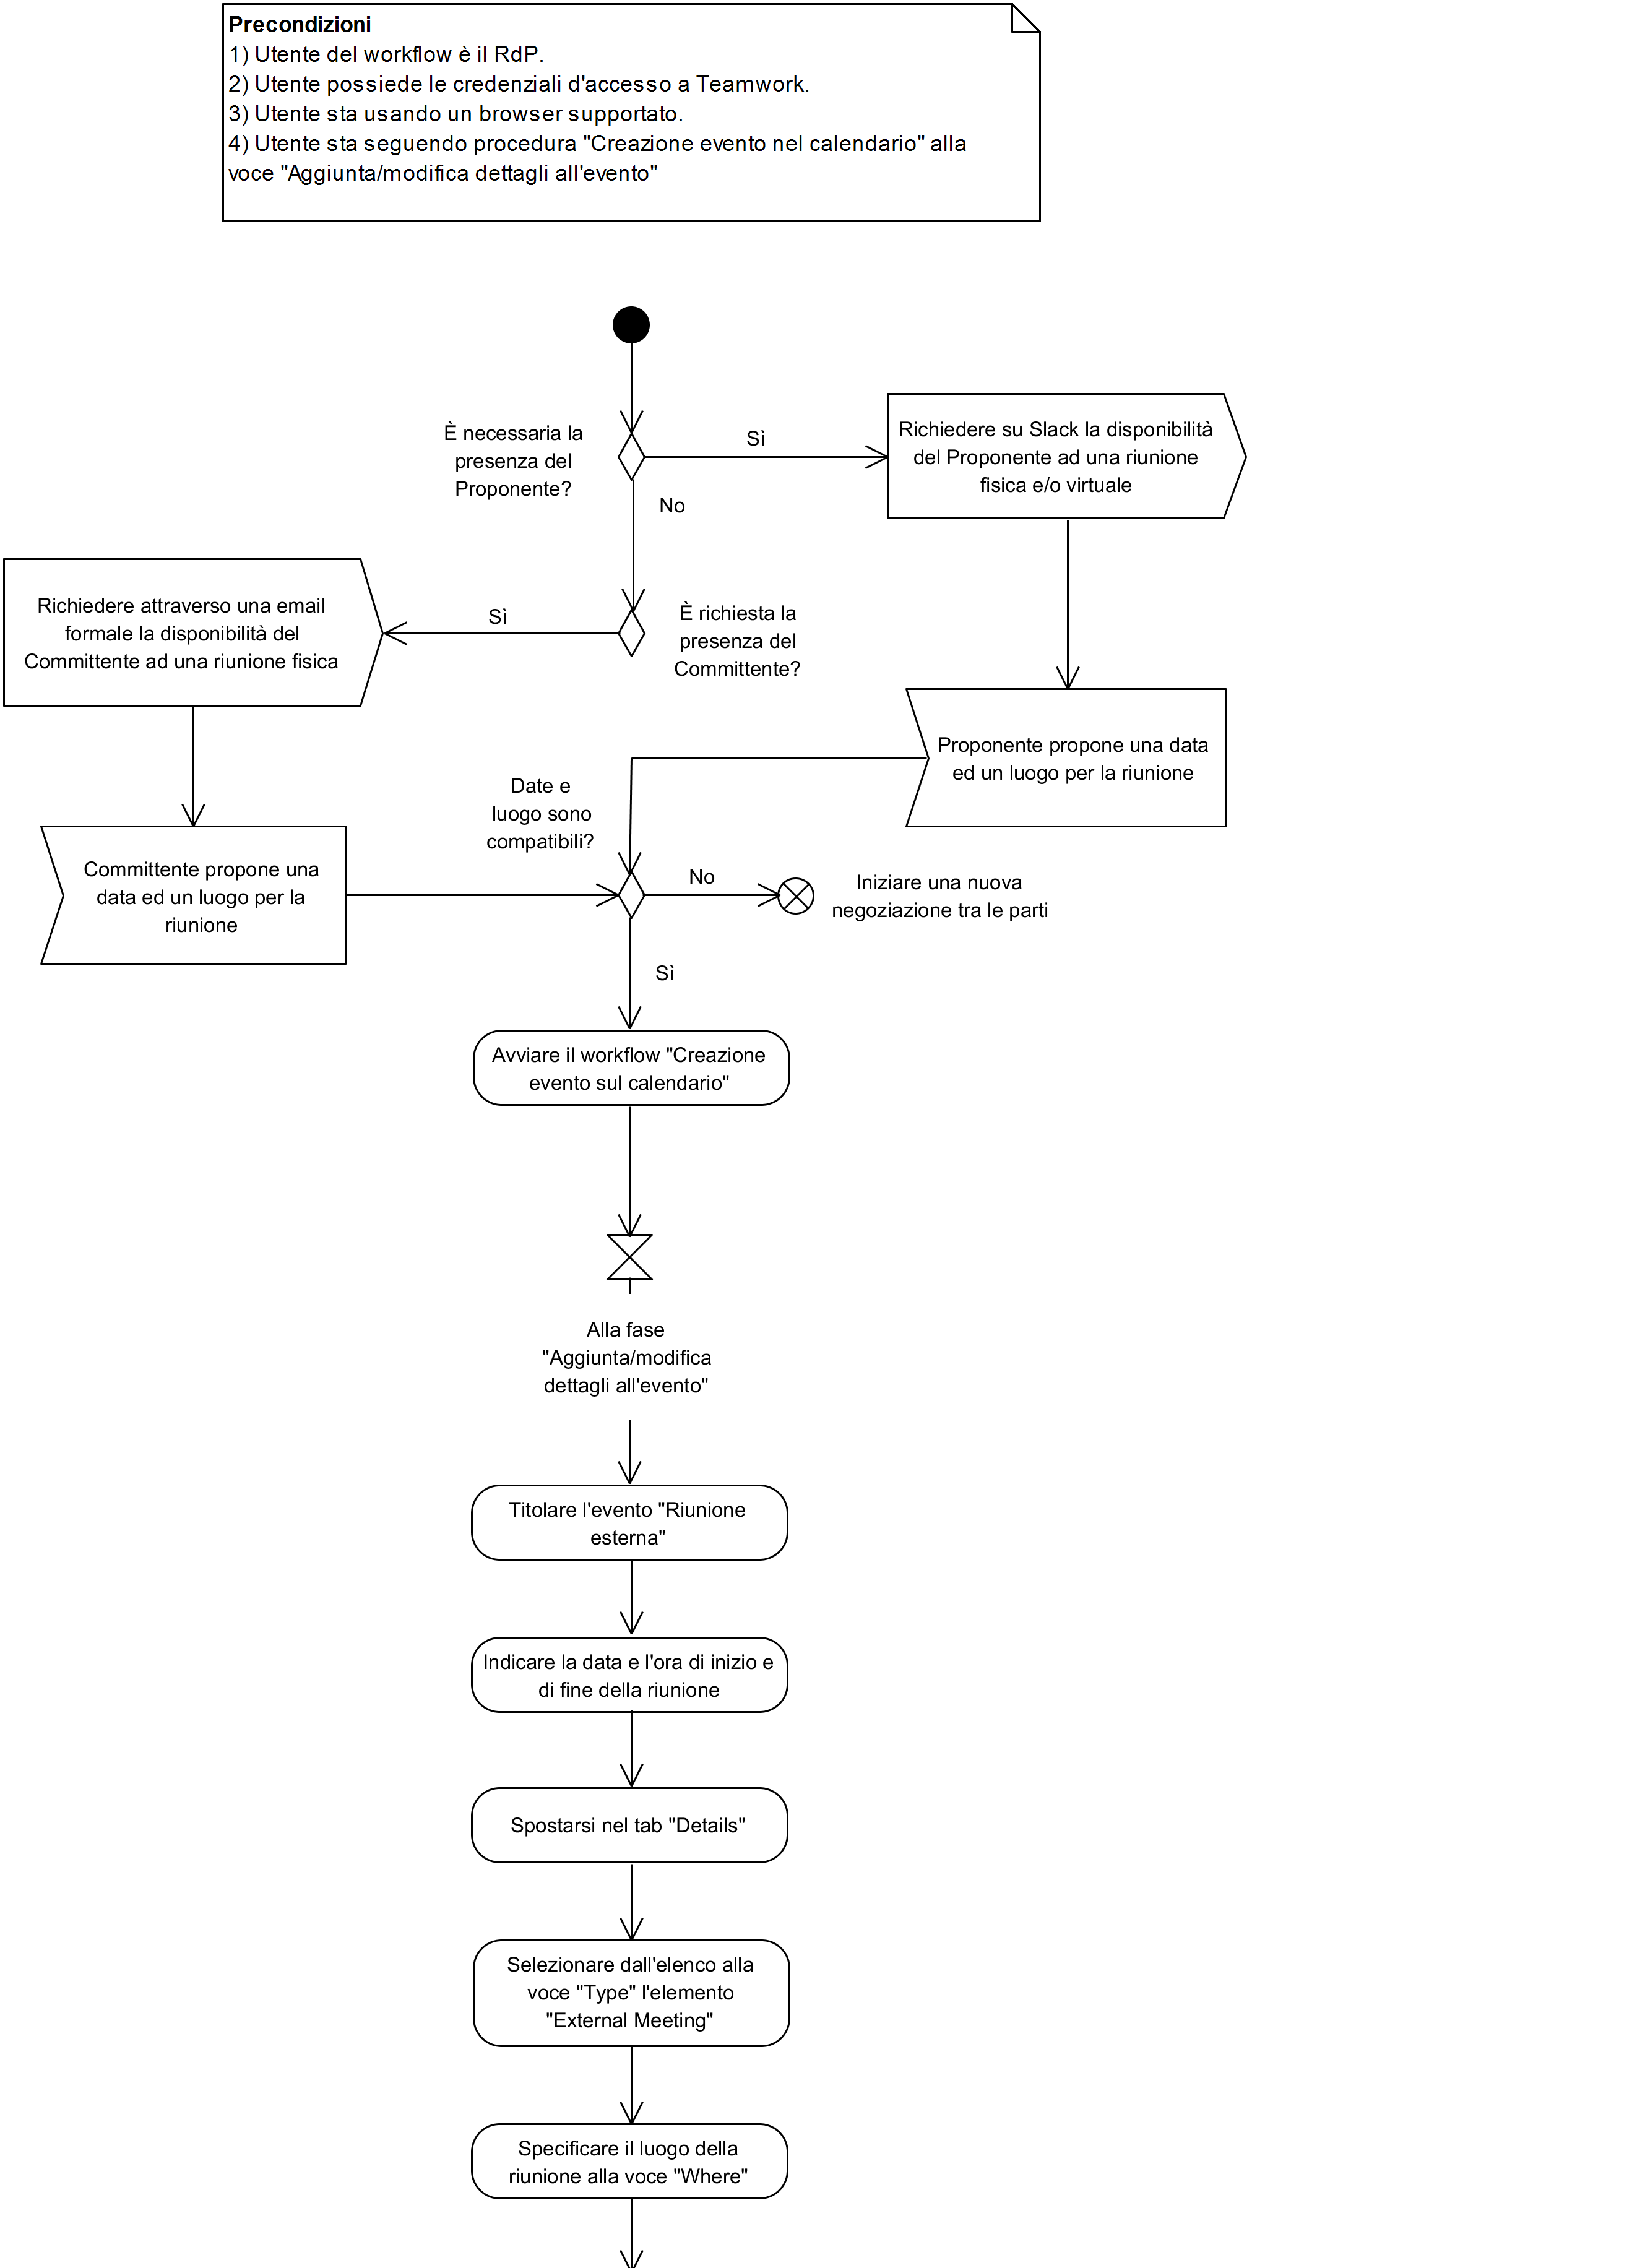
\includegraphics[width=14cm]{../../documenti/NormeDiProgetto/DiagrammiProcedure/RiunioneEsterna1.png}
	\captionof{figure}{Procedura di creazione di una riunione esterna - Parte 1}
\end{center}

\begin{center}
	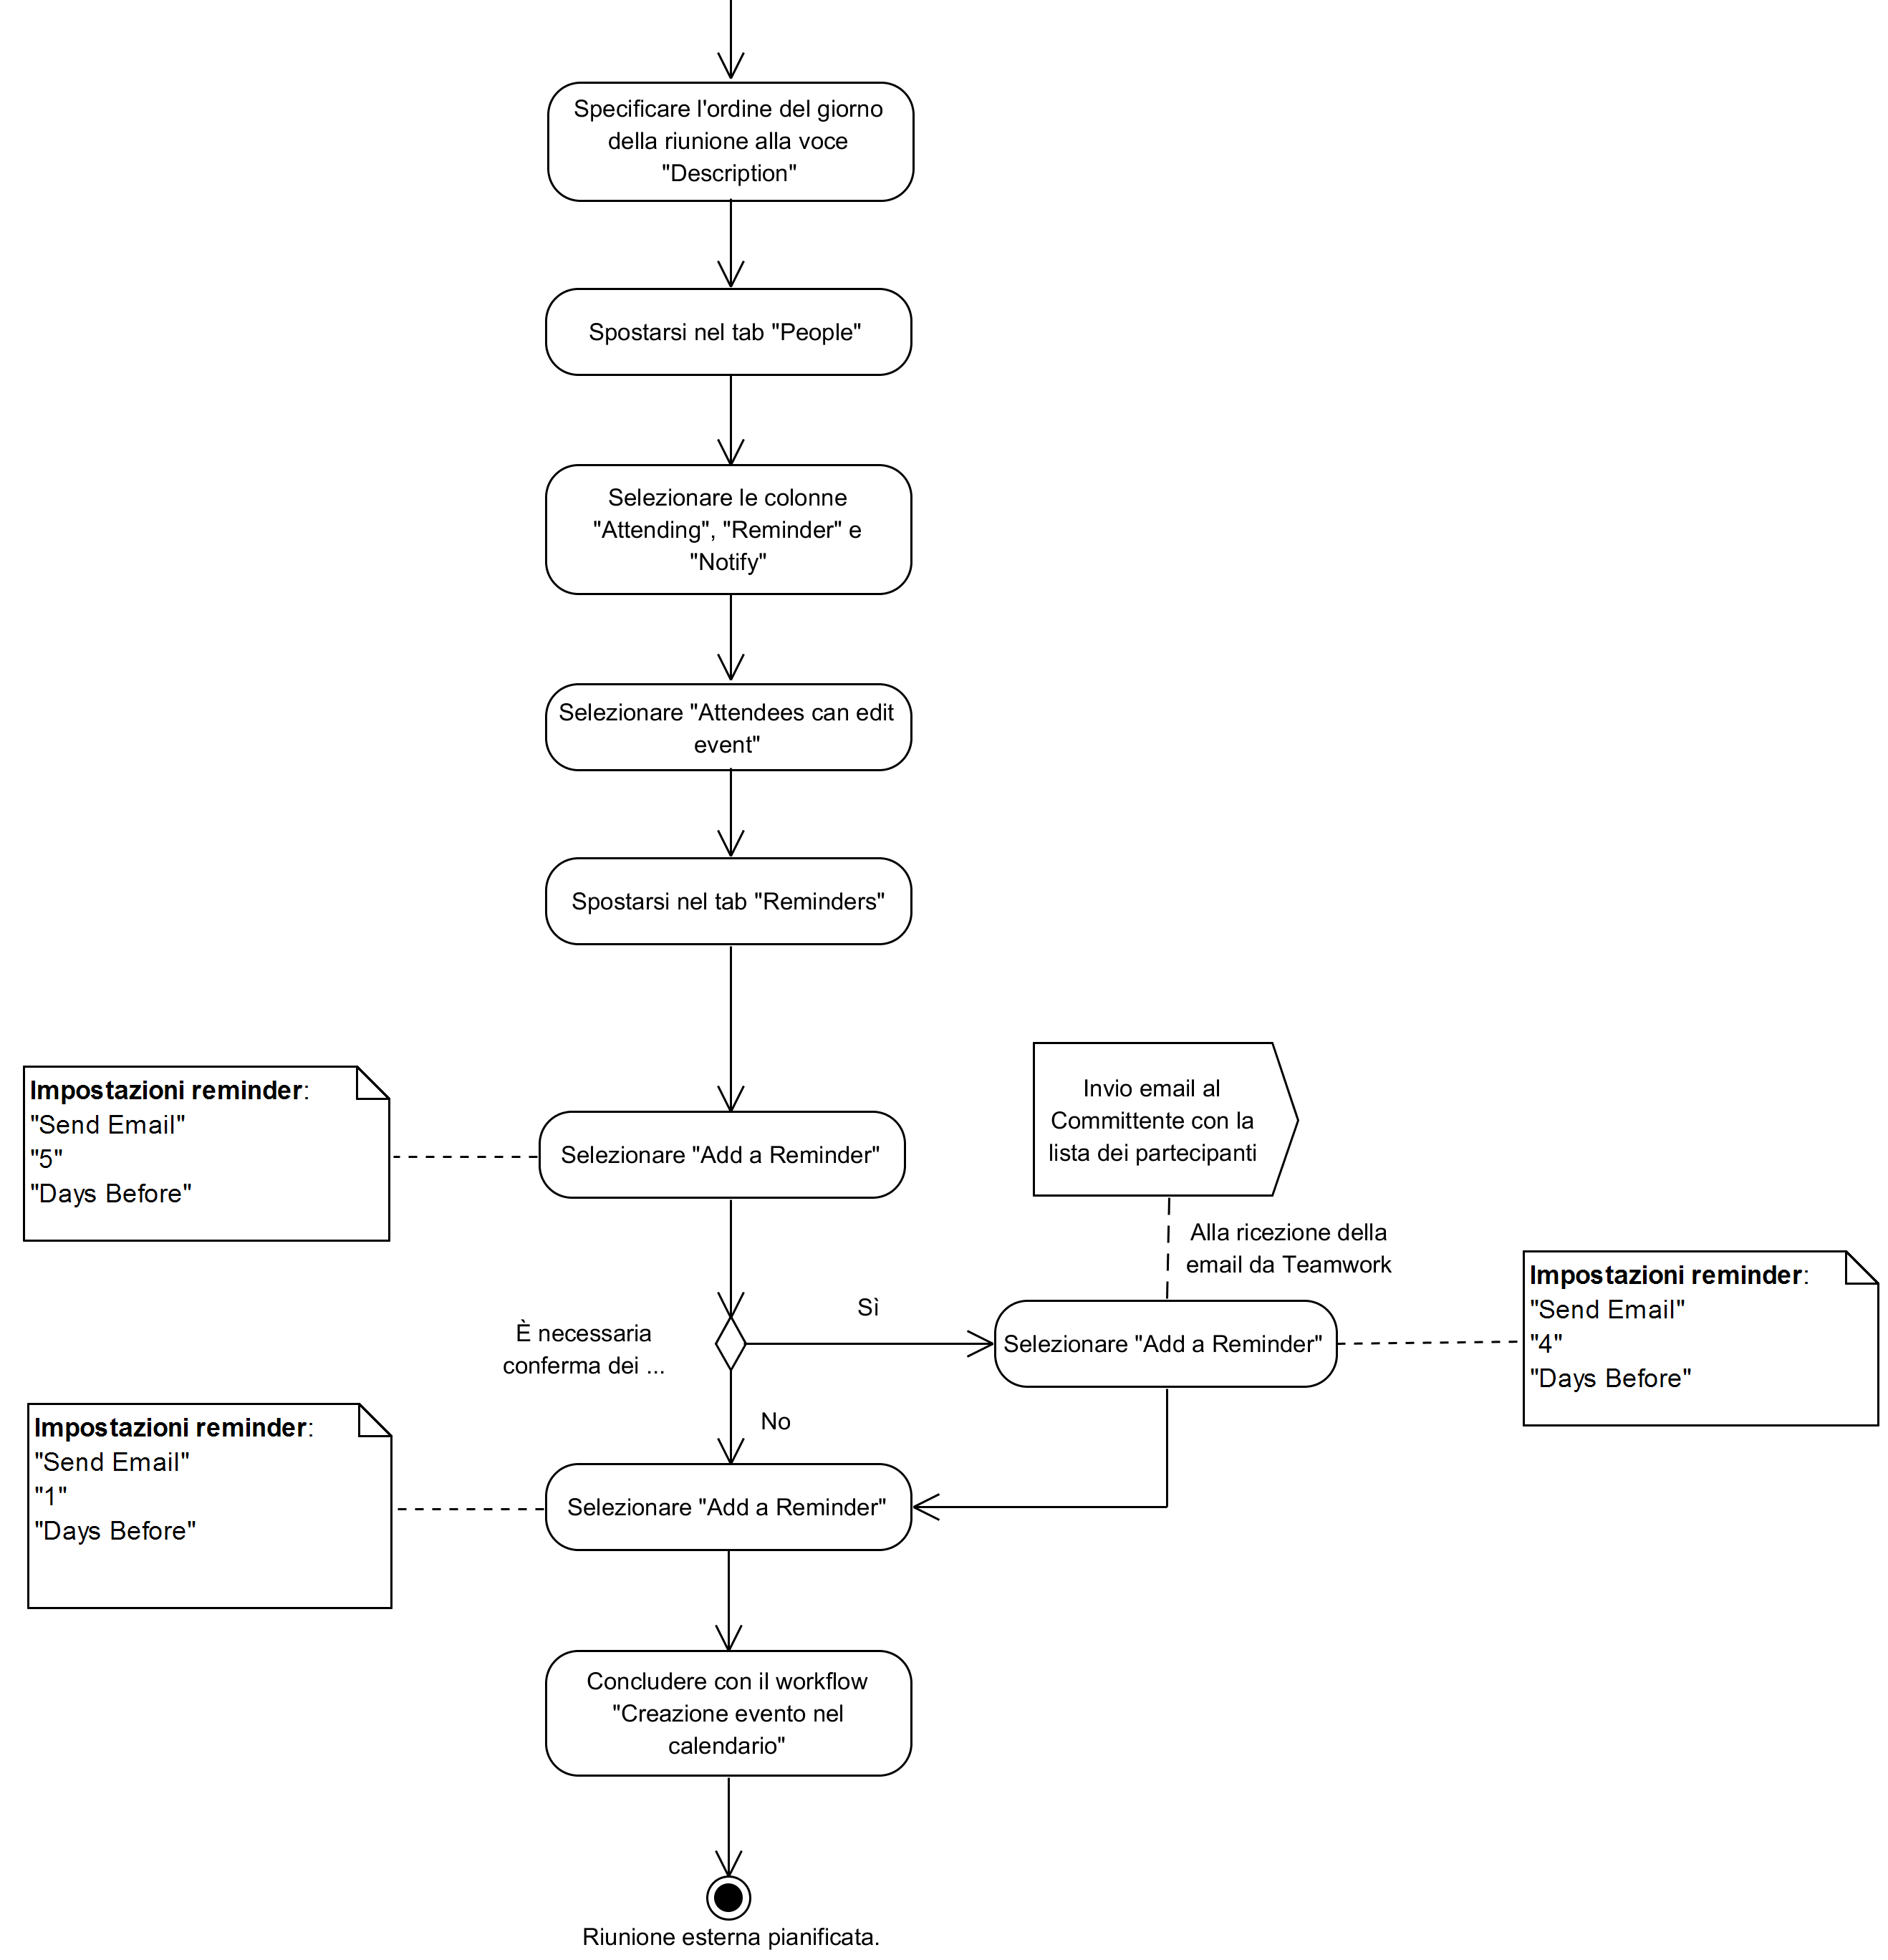
\includegraphics[width=15cm]{../../documenti/NormeDiProgetto/DiagrammiProcedure/RiunioneEsterna2.png}
	\captionof{figure}{Procedura di creazione di una riunione esterna - Parte 2}
\end{center}

\paragraph{Procedura di segnalazione di assenza da un evento:}

\begin{center}
	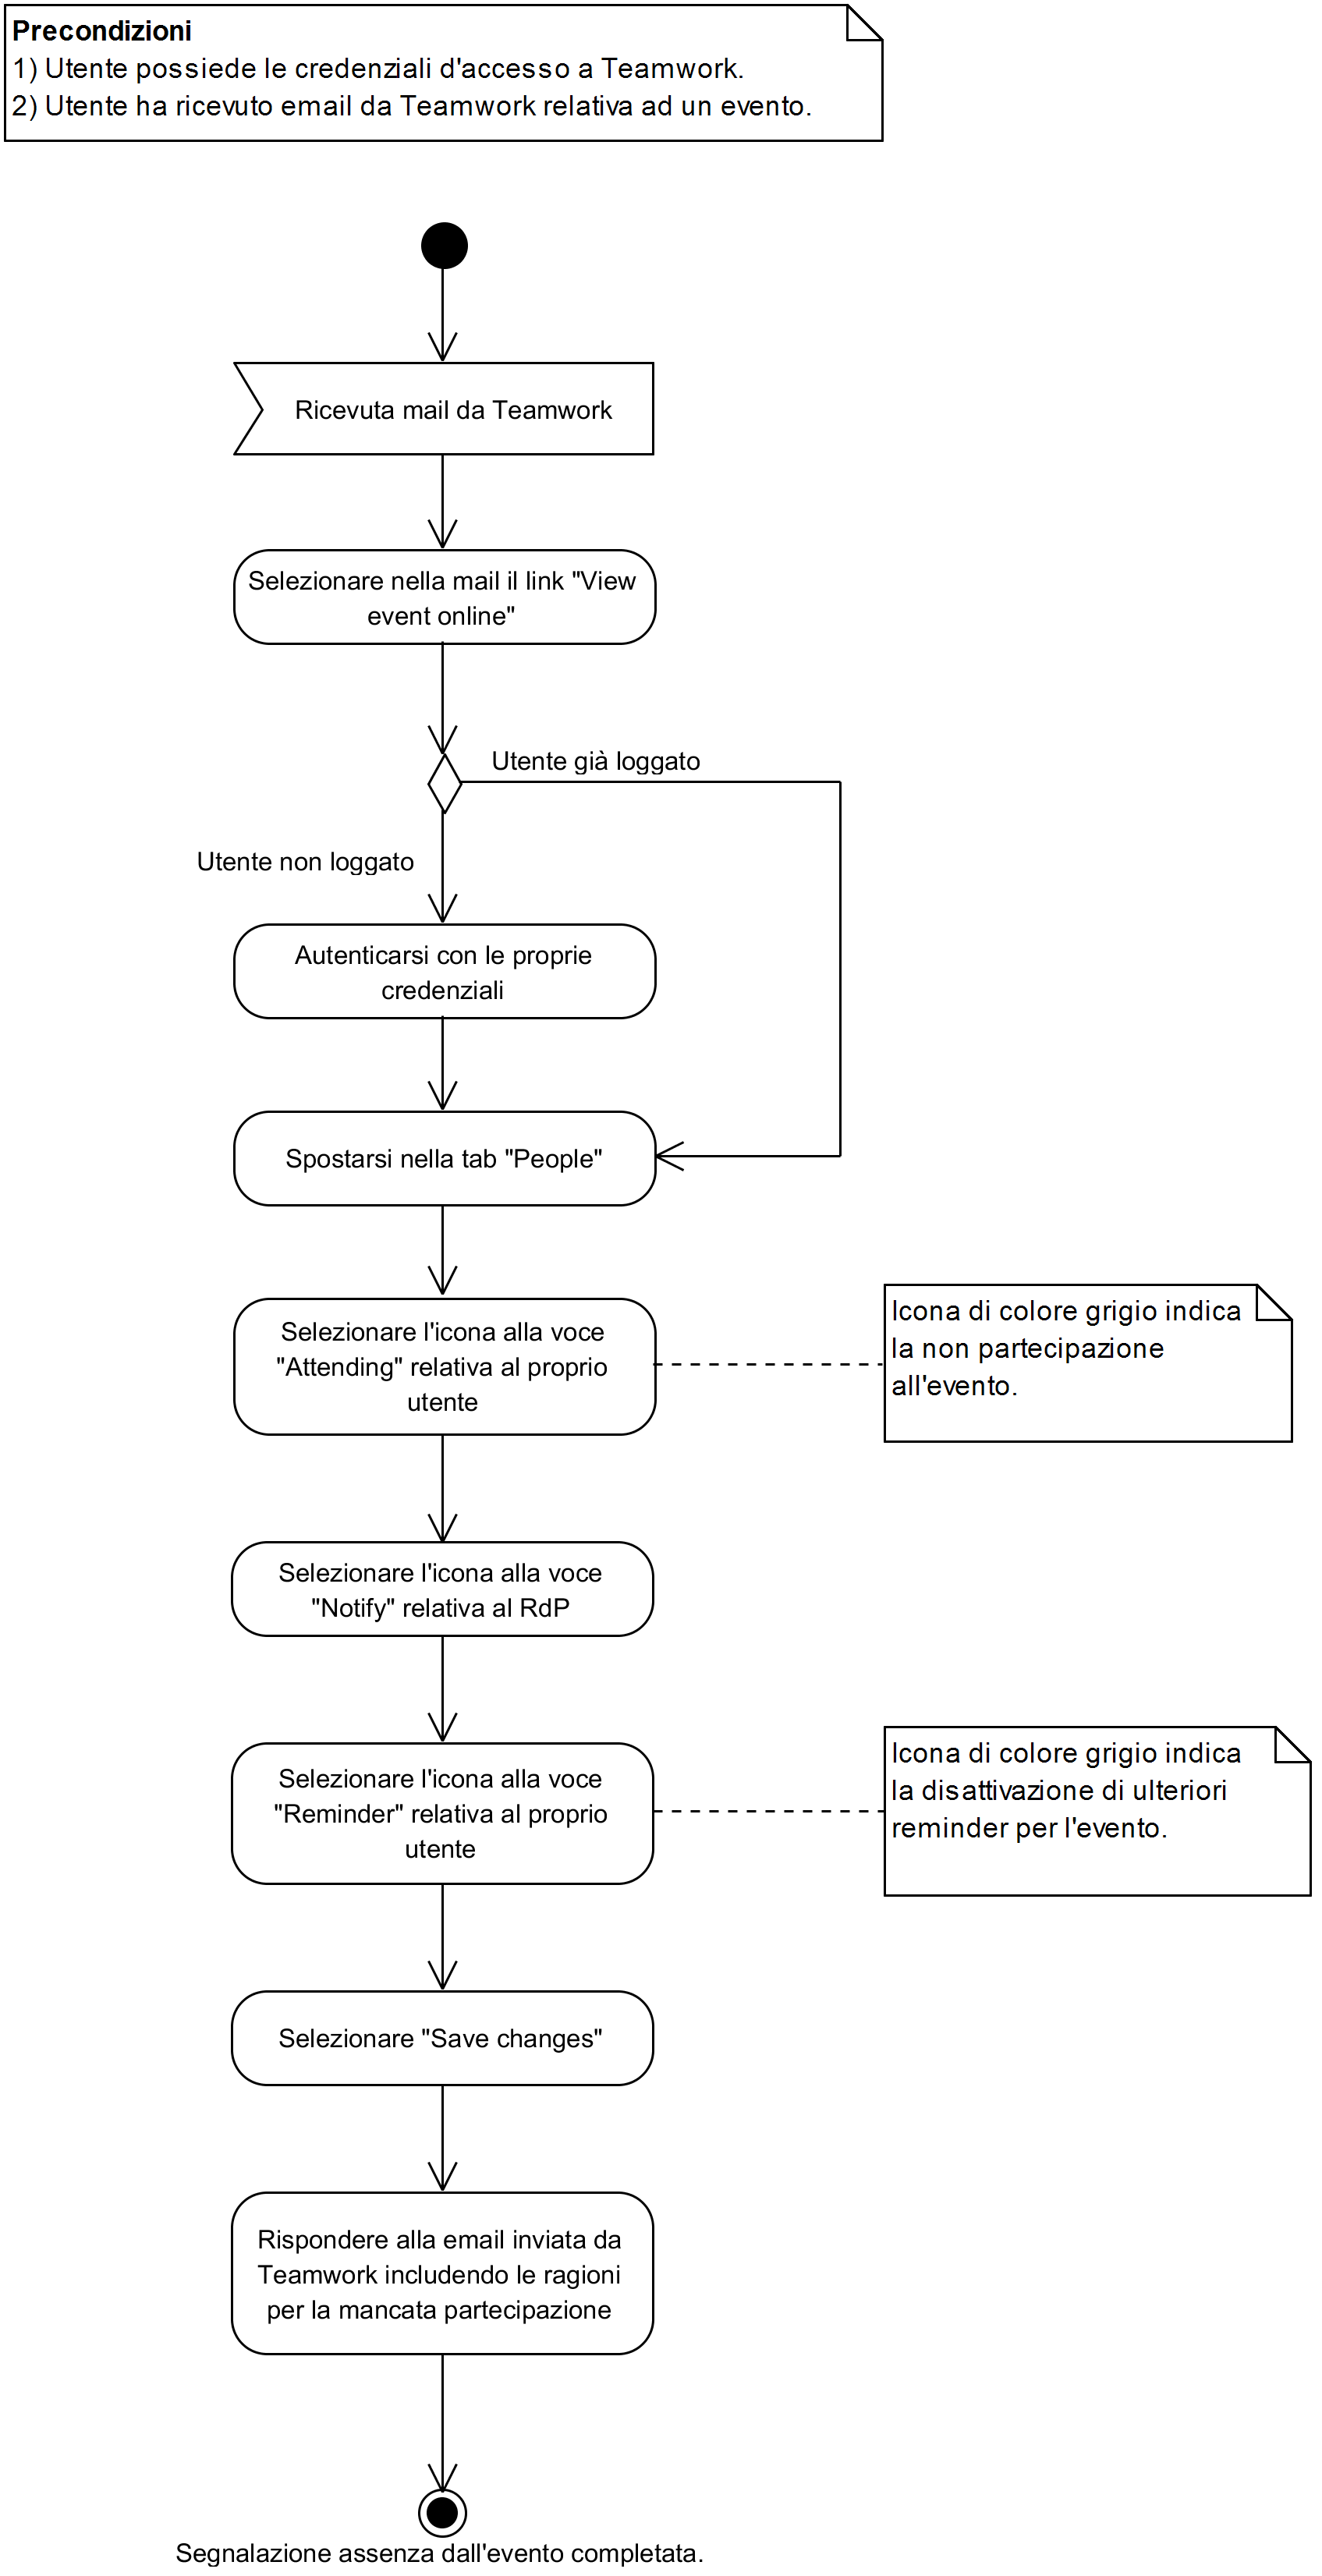
\includegraphics[width=10cm]{../../documenti/NormeDiProgetto/DiagrammiProcedure/SegnalazioneAssenzaDaUnEvento.png}
	\captionof{figure}{Procedura di segnalazione di assenza da un evento}
\end{center}

\subsection{Software per la stesura dei documenti}
La stesura dei documenti va fatta tramite linguaggio di markup \glossario{\LaTeX{}}, integrato con \glossario{Google Documents} per la scrittura del contenuto. 

\subsubsection{\LaTeX}
La scelta di usare \glossario{\LaTeX{}} è stata determinata dalla possibilità di separare il contenuto dalla formattazione, che questo strumento propone in maniera automatica tramite l'utilizzo di costrutti e template. Questi ultimi sono inoltre condivisibili tra documenti diversi, semplificando così il lavoro di aggiornamento e mantenimento di contenuti condivisi, come le versioni dei documenti, il nome del gruppo e altro ancora.

\paragraph{TeXstudio}\mbox{}\\
\`{E} stato scelto \glossario{TeXstudio} come editor per \glossario{\LaTeX{}} in quanto offre funzionalità complete ed è quello con aggiornamenti più recenti. Sono stati valutati altri editor, tra cui \glossario{TeXMaker} e \glossario{Overleaf}, ma dopo una attenta analisi sono stati scartati. Più precisamente la versione gratuita di \glossario{Overleaf} limitava il numero di progetti e lo spazio disponibile per il salvataggio di documenti nel cloud offerto, sebbene esso offrisse la possibilità di lavorare contemporaneamente su uno stesso documento in real-time. \glossario{TeXMaker} invece non offriva nulla di più di \glossario{TeXstudio}, e risultava meno aggiornato.

\paragraph{Google Documents}\mbox{}\\
Questo strumento è stato scelto per emulare la funzionalità di collaborazione offerta da \glossario{Overleaf}. In particolare viene utilizzato per la stesura del contenuto dei documenti in maniera collaborativa, sfruttando gli strumenti di comunicazione vocale e testuale. \glossario{Google Documents} permette inoltre di tenere traccia delle modifiche fatte da ogni componente, tramite cronologia delle modifiche, e di commentare parti di testo. 

\subsubsection{Diagrammi UML}
Per la modellazione \glossario{UML} è stato scelto di utilizzare \textbf{\glossario{Visual Paradigm}}, disponibile in versione gratuita per \glossario{Windows}, \glossario{MacOs} e \glossario{Linux}. \`{E} uno strumento completo e già conosciuto da alcuni componenti del gruppo. Permette di creare in modo intuitivo diagrammi \glossario{UML} e di esportarli in file immagini, condivisibili e visualizzabili rapidamente attraverso gli strumenti di comunicazione, oltre che integrabili direttamente nei documenti di testo.

\subsection{Fogli di calcolo} \label{sec:fogli_di_calcolo}
\paragraph{Google Sheets}\mbox{}\\
L'elaborazione dei dati avviene tramite \glossario{Google Sheets}, in quanto permette la collaborazione real-time tra i componenti del gruppo. Vengono prodotti con questo software:
	\begin{itemize}
	\item tabelle orarie e dei costi per il calcolo del preventivo;
	\item tabelle di confronto tra preventivo e consuntivo.
	\end{itemize}

\paragraph{Microsoft Excel} \mbox{}\\
Viene usato per creare grafici personalizzati ed esportarli nei formati immagine. Queste funzionalità sono supportate in modo parziale o nullo in \glossario{Google Sheets}.

\subsection{Tecnologie utilizzate}
\subsubsection{JavaScript}
JavaScript è un linguaggio di scripting orientato agli oggetti e agli eventi. Viene comunemente utilizzato nella programmazione web lato client per aggiungere interattività a pagine web.\\
Le caratteristiche principali di JavaScript sono:
\begin{itemize}
	\item è un linguaggio interpretato: il codice non viene compilato, ma interpretato;
	\item definisce le funzionalità tipiche dei linguaggi di programmazione ad alto livello e consente l'utilizzo del paradigma object oriented;
	\item è un linguaggio debolmente tipizzato;
	\item il codice viene eseguito direttamente sul client e non sul server: il vantaggio di questo approccio è che, anche con la presenza di script particolarmente complessi, il web server non viene sovraccaricato a causa delle richieste dei client.
\end{itemize}
Lo standard utilizzato per questo progetto è \glossario{ECMAScript} 6 con un approccio \glossario{promise}.
Il \glossario{framework} e la demo del prodotto finale sono scritti in \glossario{JavaScript}.

\paragraph{Meteor}\mbox{}\\
\glossario{Meteor} è una piattaforma \glossario{JavaScript} \glossario{full-stack} per lo sviluppo di applicazioni web e mobile moderne. Include un set di tecnologie chiave per costruire applicazioni \glossario{reactive}, uno \glossario{strumento di build} e un set di pacchetti offerti dalla community \glossario{Node.js} e \glossario{JavaScript}.\\
\glossario{Meteor} permette di sviluppare in un solo linguaggio, \glossario{JavaScript}, in tutti gli ambienti: applicazioni server, browser web e dispositivi mobile.\\
In \glossario{Meteor} il server invia dati e non \glossario{HTML}, mentre il client li renderizza.
Alcune caratteristiche di \glossario{Meteor} sono:
\begin{itemize}
	\item isomorfismo: il codice viene eseguito sia lato server che lato client;
	\item reattività: l'interfaccia utente rispecchia il reale stato delle variabili con uno sforzo di sviluppo minimale.
\end{itemize}

\paragraph{React}\mbox{}\\
\glossario{React} è una libreria \glossario{JavaScript} per la costruzione di interfacce utente dinamiche e complesse, ma dall'utilizzo semplice e intuitivo. \`{E} alla base del frontend di Facebook, dal quale è stata creata.\\
\glossario{React} consente l'uso di un approccio dichiarativo simile all'\glossario{HTML} per definire i componenti che rappresentano parti significative e logiche dell'interfaccia utente. Nonostante ciò, la rappresentazione del componente in realtà si traduce in chiamate all'\glossario{API} di \glossario{React} che intervengono sul \glossario{DOM} della pagina per creare gli elementi necessari.

\subsubsection{SCSS (Sass 3)}
\glossario{Sass} (Syntactically Awesome StyleSheets) è un'estensione del linguaggio \glossario{CSS} che permette di utilizzare variabili, di creare funzioni e di organizzare il foglio di stile in più file.\\
Il linguaggio \glossario{Sass} si basa sul concetto di preprocessore \glossario{CSS}, il quale serve a definire fogli di stile con una forma più semplice, completa e potente rispetto ai \glossario{CSS} e a generare file \glossario{CSS} ottimizzati, aggregando le strutture definite anche in modo complesso.\\
\glossario{SCSS} è la versione 3 di \glossario{Sass} e la sua sintassi è basata completamente su \glossario{CSS}. In questo modo è garantita la compatibilità di \glossario{CSS} verso \glossario{SCSS}.

\subsubsection{Rocket.Chat}
\glossario{Rocket.Chat} è una piattaforma di messaggistica open-source, ispirata a \glossario{Slack}. \`{E} un servizio multi piattaforma, accessibile tramite browser e applicazione desktop e mobile. \`{E} altamente personalizzabile in quanto, oltre ad essere su un \glossario{repository} pubblico, è espandibile tramite pacchetti disponibili online. Alcune funzionalità base di \glossario{Rocket.Chat} sono:
\begin{itemize}
	\item livechat;
	\item conferenze video;
	\item condivisione di file;
	\item \glossario{TeX rendering} di formule matematiche;
	\item condivisione dello schermo;
	\item integrazione con servizi esterni (\glossario{GitHub}, \glossario{GitLab}, \glossario{Jira} ad esempio);
	\item estendibilità tramite pacchetti sviluppabili da chiunque.
\end{itemize}

\subsection{Strumenti per lo sviluppo dell'applicazione}
\textbf{\glossario{Heroku}} è un \glossario{Platform-as-a-Service} (PaaS) su cloud basato sul concetto di contenitori, che permette di sviluppare applicazioni in modo indipendente dall'ambiente di sviluppo dei singoli membri del gruppo. \`{E} integrabile con \glossario{Git} e con i sistemi di integrazione continua e pertanto permette un approccio \virgolette{app-centric} e la scalabilità delle applicazioni.\\
\`{E} stato preso in considerazione anche \glossario{Docker}, per lo stesso scopo, ma è stato scartato in quanto presenta alcuni problemi di gestione e configurazione dell'ambiente run-time, oltre ad essere stato sconsigliato dal Proponente, mentre vi è un esplicito riferimento ad \glossario{Heroku} nel capitolato.

\subsection{Strumenti per la documentazione}
Come strumento di generazione per la documentazione del codice è stato scelto \textbf{\glossario{Meteor-JSDoc}}.\\
\glossario{Meteor-JSDoc} fa uso della versione in sviluppo di \textbf{\glossario{JSDoc}} per fornire maggior supporto alla nuova sintassi \glossario{JavaScript}.
\glossario{JSDoc} è un generatore di documentazione delle \glossario{API} per \glossario{JavaScript}. Aggiungendo commenti che documentino il codice direttamente all'interno dei sorgenti, questo strumento analizza il codice e genera una documentazione completa in formato \glossario{HTML}.
Alcune caratteristiche di \glossario{Meteor-JSDoc} sono:
\begin{itemize}
	\item è basato sui template della documentazione stessa di \glossario{Meteor};
	\item la documentazione prodotta è usata anche dall'applicazione \glossario{Meteor}, che la mostra ben formattata per l'applicazione creata;
	\item supporta il collegamento al \glossario{repository} \glossario{GitHub}.
\end{itemize}

\subsection{Strumenti per la codifica}
L'\glossario{IDE} scelto per l'attività di codifica è \textbf{\glossario{WebStorm}}. Esso è disponibile in versione gratuita ed è compreso nel pacchetto studenti offerto da \glossario{JetBrains}. Alcune funzionalità che rende disponibili sono:
\begin{itemize}
	\item assistenza nella codifica per \glossario{React}, \glossario{Meteor} e \glossario{CSS};
	\item supporto di \glossario{Cordova} per lo sviluppo mobile e \glossario{Node.js} per il lato server;
	\item autocompletamento di metodi, funzioni e \glossario{framework} esterni;
	\item debugger integrato;
	\item test di unità tramite \glossario{Mocha};
	\item tracciamento del codice \glossario{JavaScript};
	\item integrazione con \glossario{npm};
	\item strumenti per la qualità integrati, tra cui \glossario{ESLint};
	\item sistema di versionamento integrato, sia per cambiamenti locali, sia per servizi esterni, tra i quali \glossario{GitHub}.
\end{itemize}

\subsection{Strumenti per la verifica}
\subsubsection{Script}
Vengono utilizzati degli script per il calcolo degli indici di leggibilità dei documenti.

\subsubsection{Test di integrazione}
\paragraph{Mocha}\mbox{}\\
\glossario{Mocha} è un \glossario{framework} per il testing di codice \glossario{JavaScript}, eseguibile su \glossario{Node.js} e nel browser. I test di \glossario{Mocha} vengono eseguiti in modo seriale, permettendo un controllo flessibile e accurato, mentre vengono mappate le eccezioni non rilevate al corretto test.\\
Una funzionalità chiave offerta da questo \glossario{framework} è il supporto all’elaborazione asincrona, incluse le \glossario{promise}.

\paragraph{\glossario{Chai}}\mbox{}\\
\glossario{Chai} è una libreria \glossario{BDD/TDD} per \glossario{Node.js} ed il browser che può essere accoppiata con qualunque \glossario{framework} di testing per \glossario{JavaScript}.\\
Il vantaggio che questa libreria offre è la possibilità di scrivere test facilmente leggibili, in quanto molto simili al linguaggio naturale. Questo avviene grazie alla concatenazione di costrutti quali \textit{to}, \textit{be}, \textit{is}, insieme ai costrutti base \textit{expect} e \textit{should}. La concatenazione può terminare quindi con funzioni quali \textit{include} o \textit{equals}, che richiedono dei parametri in input, oppure \textit{not}, \textit{true} o \textit{false}.\\
In questo modo è possibile definire in modo chiaro il comportamento che ci si aspetta il codice abbia, o il risultato atteso dalle operazioni contenute in esso.

\subsubsection{ESLint} \label{sec:eslint}
\glossario{ESLint} è uno strumento di \glossario{linting} open source per \glossario{JavaScript}. Questo strumento permette di scovare gli errori e i problemi nel codice prodotto senza eseguirlo.\\ \glossario{ESLint} è completamente estendibile tramite plugin, pertanto permette agli sviluppatori di creare regole personalizzate.\\
In questo progetto \glossario{ESLint} viene configurato per seguire le convenzioni relative al codice descritte in \sezione{sec:convenzioni} di questo documento.
